%%%%%%%%%%%%%%%
% \setcounter{figure}{0}
% \setcounter{page}{1}
% \pagenumbering{gobble}
%%%%%%%%%%%%%%%

\begin{enumerate}
    \item Mengakses Aplikasi\label{item:mengakses-aplikasi}
    \begin{enumerate}
        \item Membuka aplikasi \textit{browser}, kemudian memasukkan tautan URL aplikasi presensi \textit{online}. \textbf{\ref{fig:memasukkan-tautan-url-melalui-browser}} menunjukkan cara memasukkan tautan URL melalui \textit{browser}.
        \begin{figure}[!htbp]
    	\centering
    	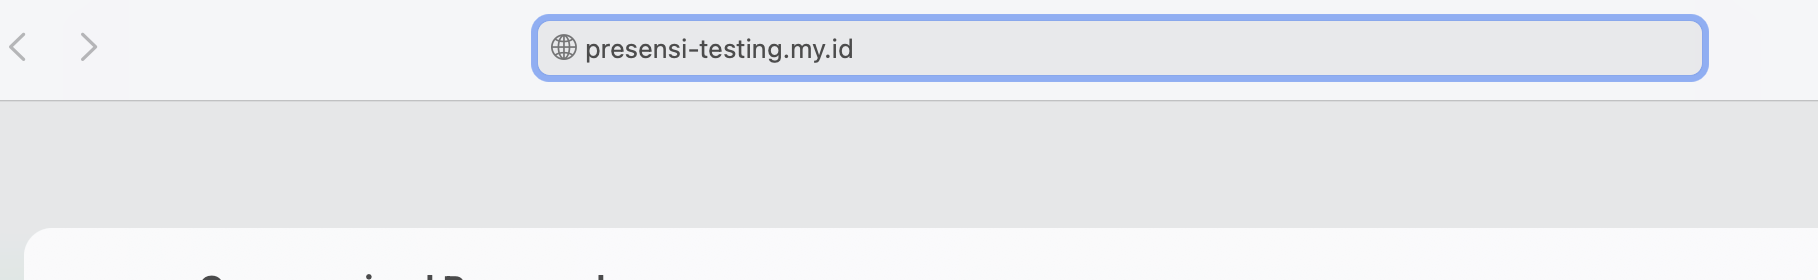
\includegraphics[width=10cm]{Gambar/bab3/user-manual/user-manual-enter-link.png}
    	\caption{Memasukkan Tautan URL Melalui \textit{Browser}}
    	\label{fig:memasukkan-tautan-url-melalui-browser}
        \end{figure}
        \FloatBarrier

        \item Setelah memasukkan tautan URL, maka halaman akan otomatis teralihkan ke halaman \textit{login} pada aplikasi presensi \textit{online}. \textbf{\ref{fig:user-manual-halaman-login}} menunjukkan tampilan \textit{login} pada aplikasi presensi \textit{online}.
        \begin{figure}[!htbp]
    	\centering
    	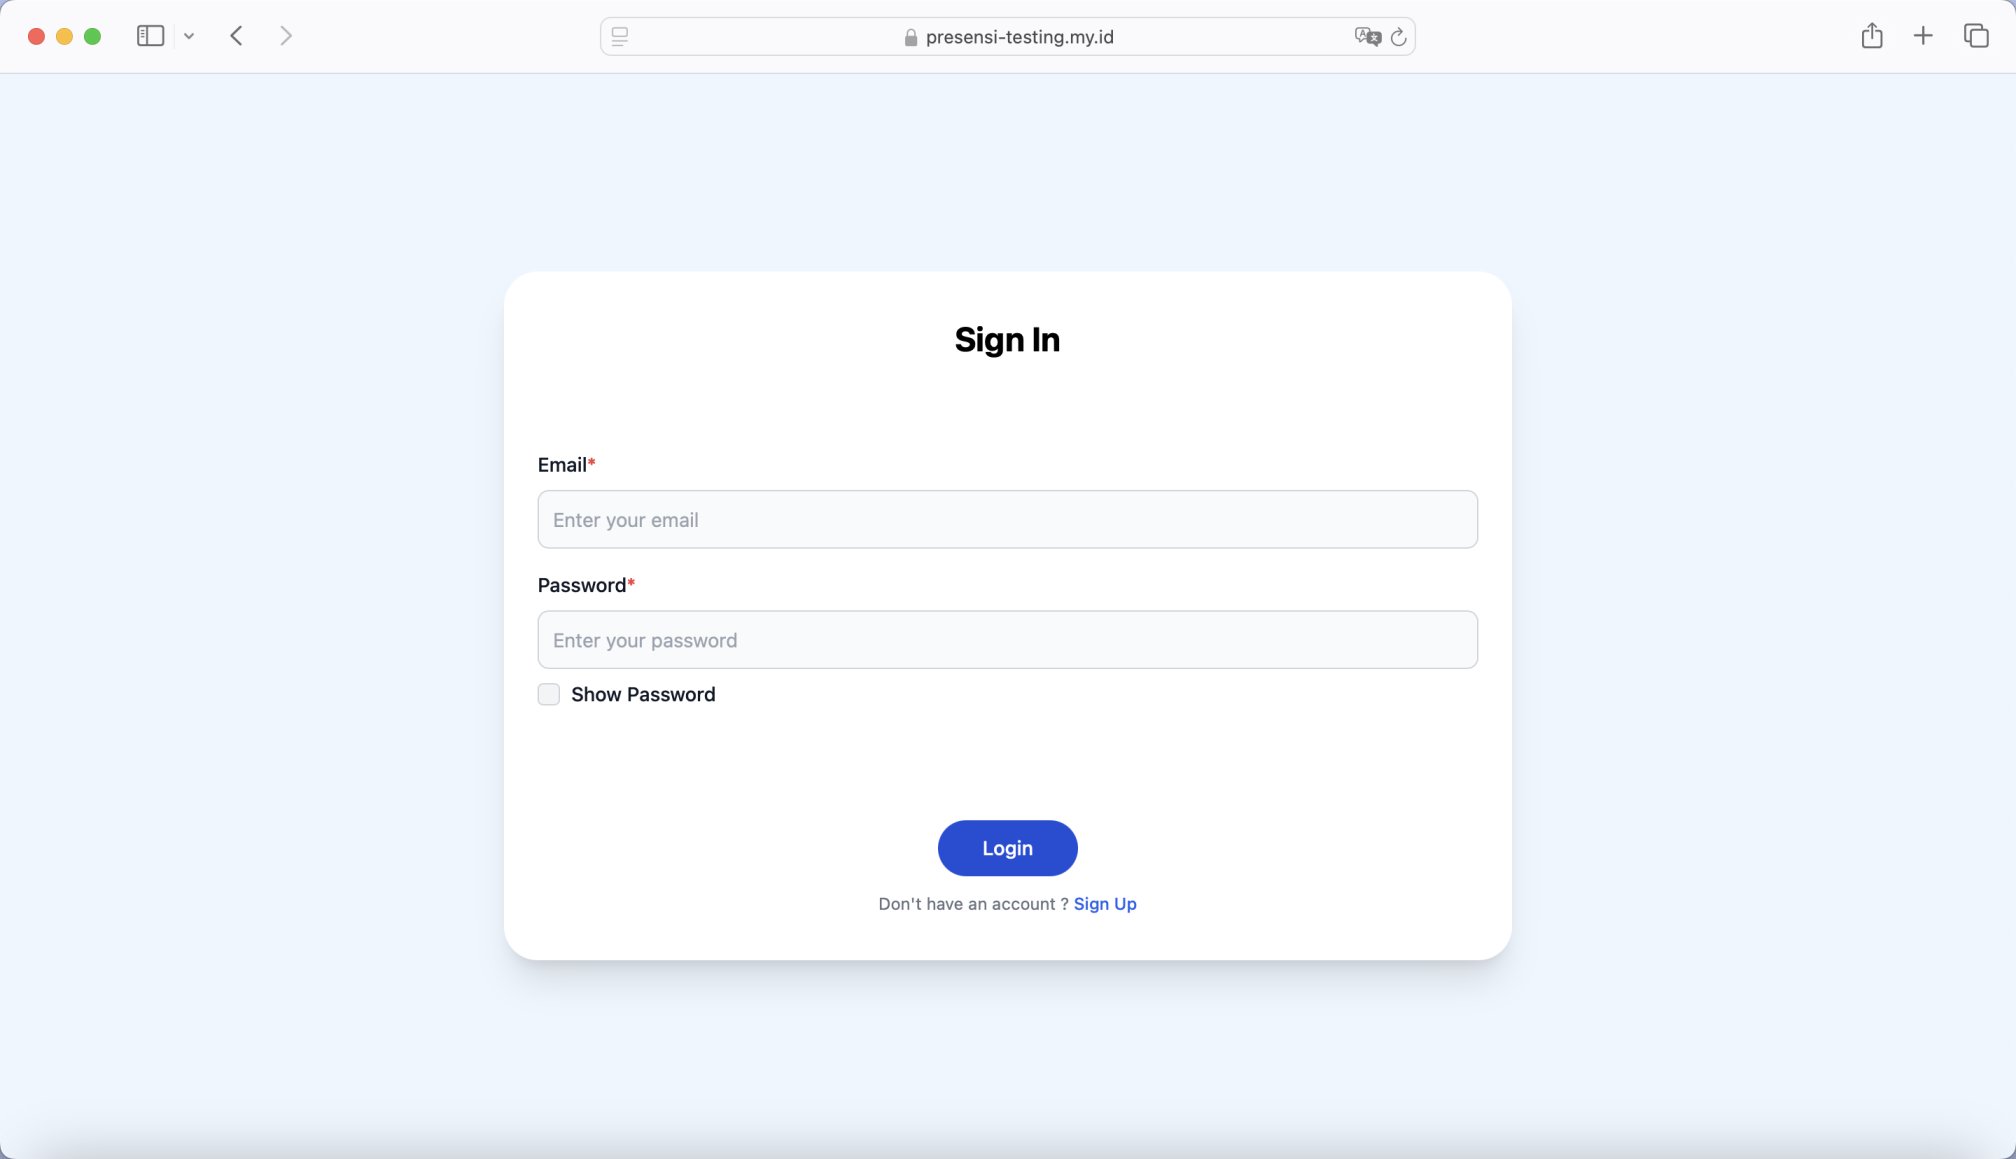
\includegraphics[width=10cm]{Gambar/bab3/user-manual/user-manual-halaman-login.png}
    	\caption{Tampilan Halaman \textit{Login}}
    	\label{fig:user-manual-halaman-login}
        \end{figure}
        \FloatBarrier
    \end{enumerate}

    \item Melakukan \textit{Login}\label{item:melakukan-login}
    \begin{enumerate}
        \item Mengakses aplikasi presensi \textit{online} yang terdapat pada \textbf{Manual \ref{item:mengakses-aplikasi}}.

        \item Mengisi seluruh \textit{input form} pada halaman \textit{login}, kemudian menekan tombol \textit{"Login"}. \textbf{\ref{fig:user-manual-halaman-login}} menunjukkan tampilan halaman \textit{login}.

        \item Halaman akan dialihkan ke halaman utama jika berhasil \textit{login}. \textbf{\ref{fig:user-manual-halaman-utama}} menunjukkan tampilan halaman utama aplikasi presensi \textit{online} ketika berhasil \textit{login}.

        \begin{figure}[!htbp]
    	\centering
    	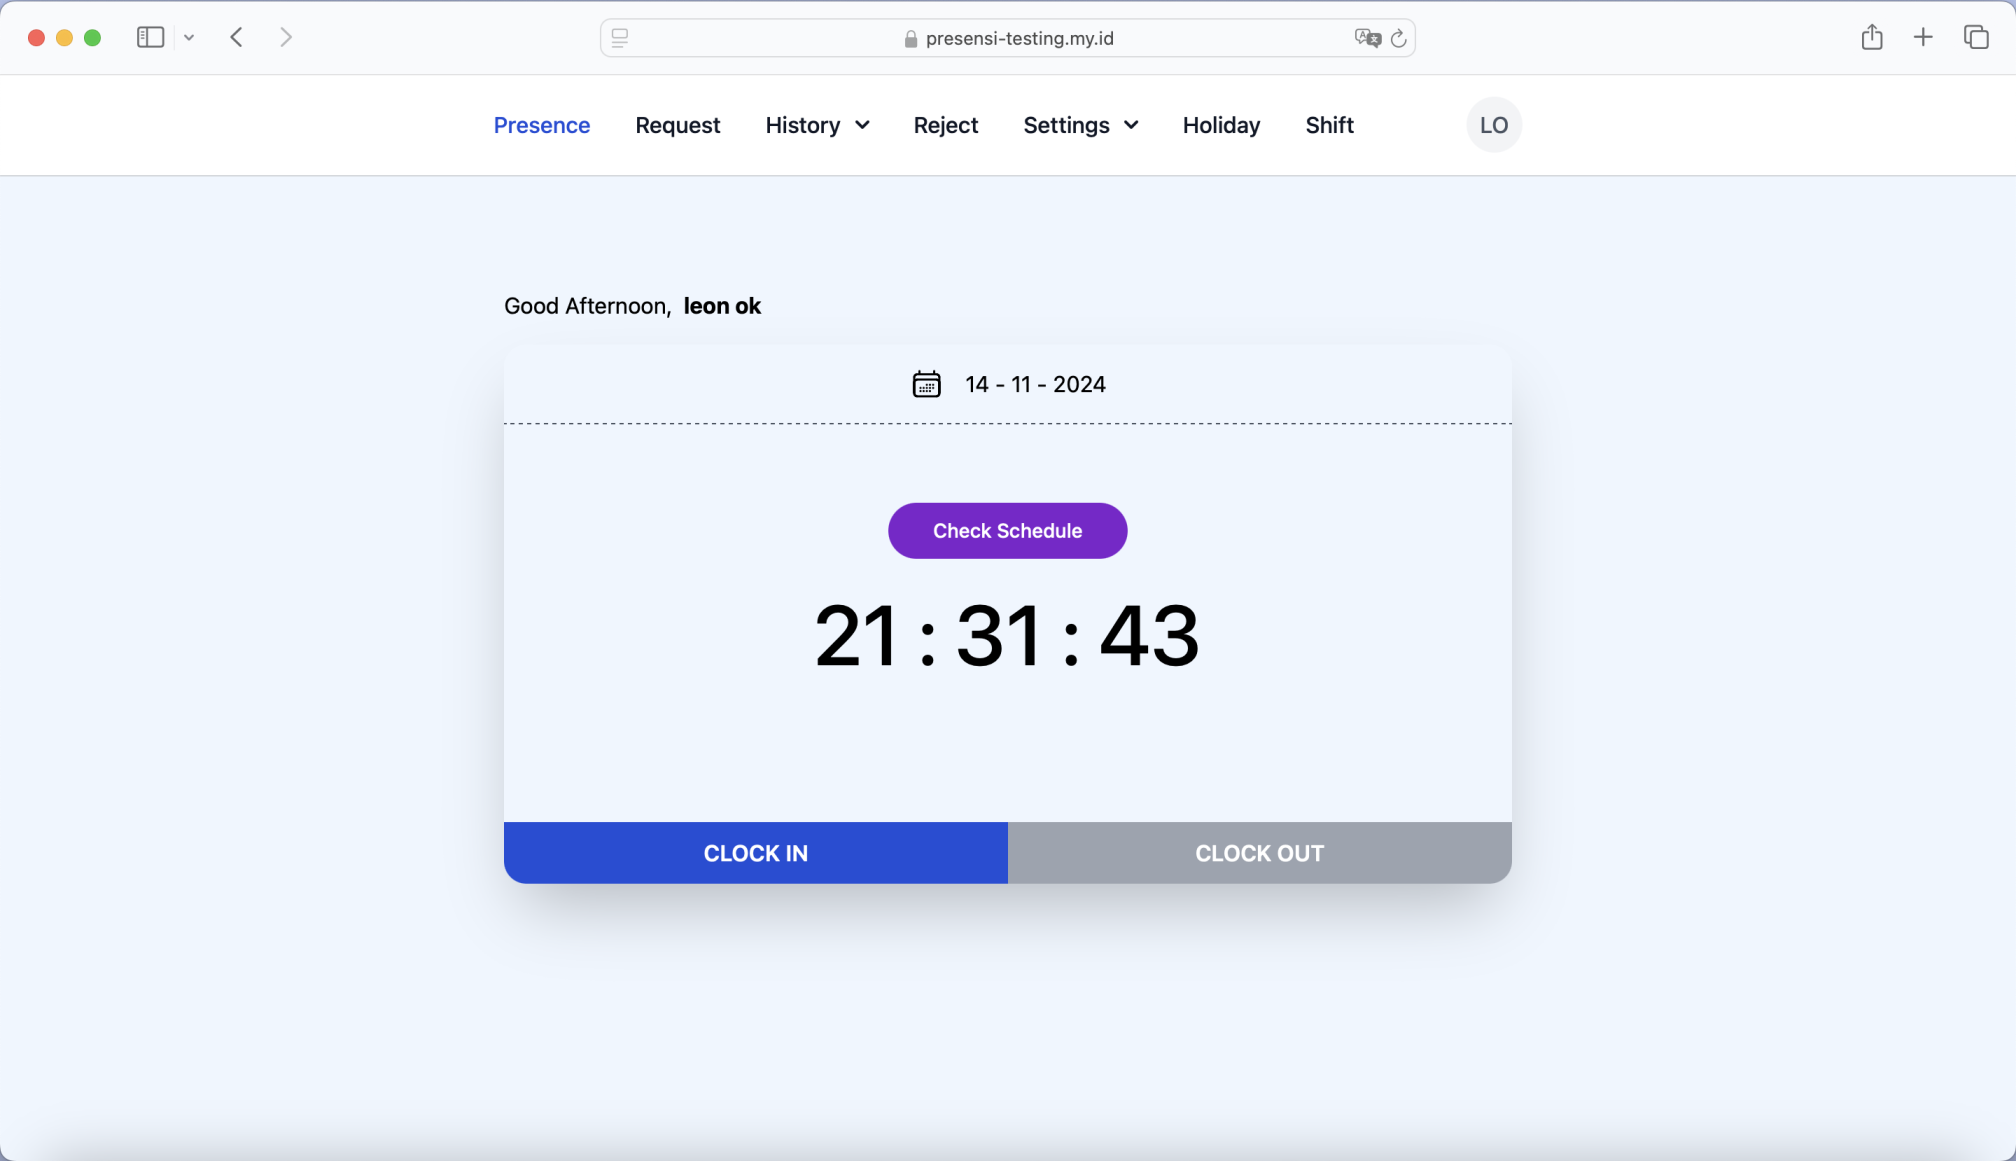
\includegraphics[width=10cm]{Gambar/bab3/user-manual/user-manual-halaman-utama.png}
    	\caption{Halaman Utama}
    	\label{fig:user-manual-halaman-utama}
        \end{figure}
        \FloatBarrier
    \end{enumerate}

    \item Melakukan Registrasi Akun
    \begin{enumerate}
        \item Mengakses aplikasi presensi \textit{online} yang terdapat pada \textbf{Manual \ref{item:mengakses-aplikasi}}.
        \item Menekan tombol \textit{"Sign Up"} pada halaman \textit{login}. \textbf{\ref{fig:user-manual-tombol-sign-up}} terdapat tombol \textit{"Sign Up"} yang terletak di paling bawah halaman.
        \item Mengisi seluruh \textit{input form} yang ada pada halaman registrasi akun dan menekan tombol \textit{"Register"}. \textbf{\ref{fig:user-manual-halaman-sign-up}} menunjukkan halaman registrasi akun.
        \item Sistem akan mengirimkan 6 digit kode OTP ke \textit{email} pengguna, memasukkan kode OTP ke dalam modal verifikasi \textit{email}. \textbf{\ref{fig:user-manual-verifikasi-email}} menunjukkan modal untuk verifikasi \textit{email} pada akun.
        \item Setelah memasukkan kode verifikasi \textit{email} dengan benar maka akan muncul pesan berhasil. \textbf{\ref{fig:user-manual-pesan-berhasil-verifikasi}} menunjukkan \textit{pop up} pesan berhasil verifikasi \textit{email} pada akun.
        \begin{figure}[!htbp]
    	\centering
    	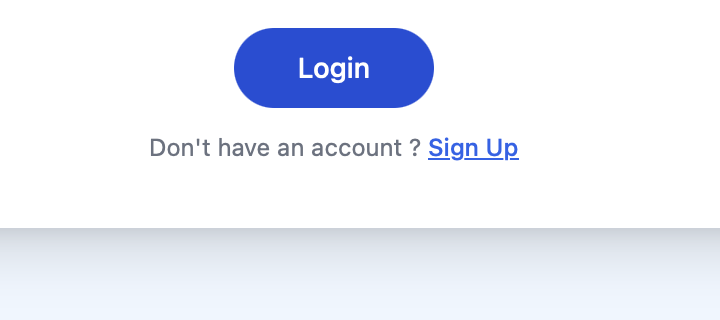
\includegraphics[width=10cm]{Gambar/bab3/user-manual/user-manual-tombol-sign-up.png}
    	\caption{Tombol \textit{Sign Up} Pada Halaman \textit{Login}}
    	\label{fig:user-manual-tombol-sign-up}
        \end{figure}
        \FloatBarrier

        \begin{figure}[!htbp]
    	\centering
    	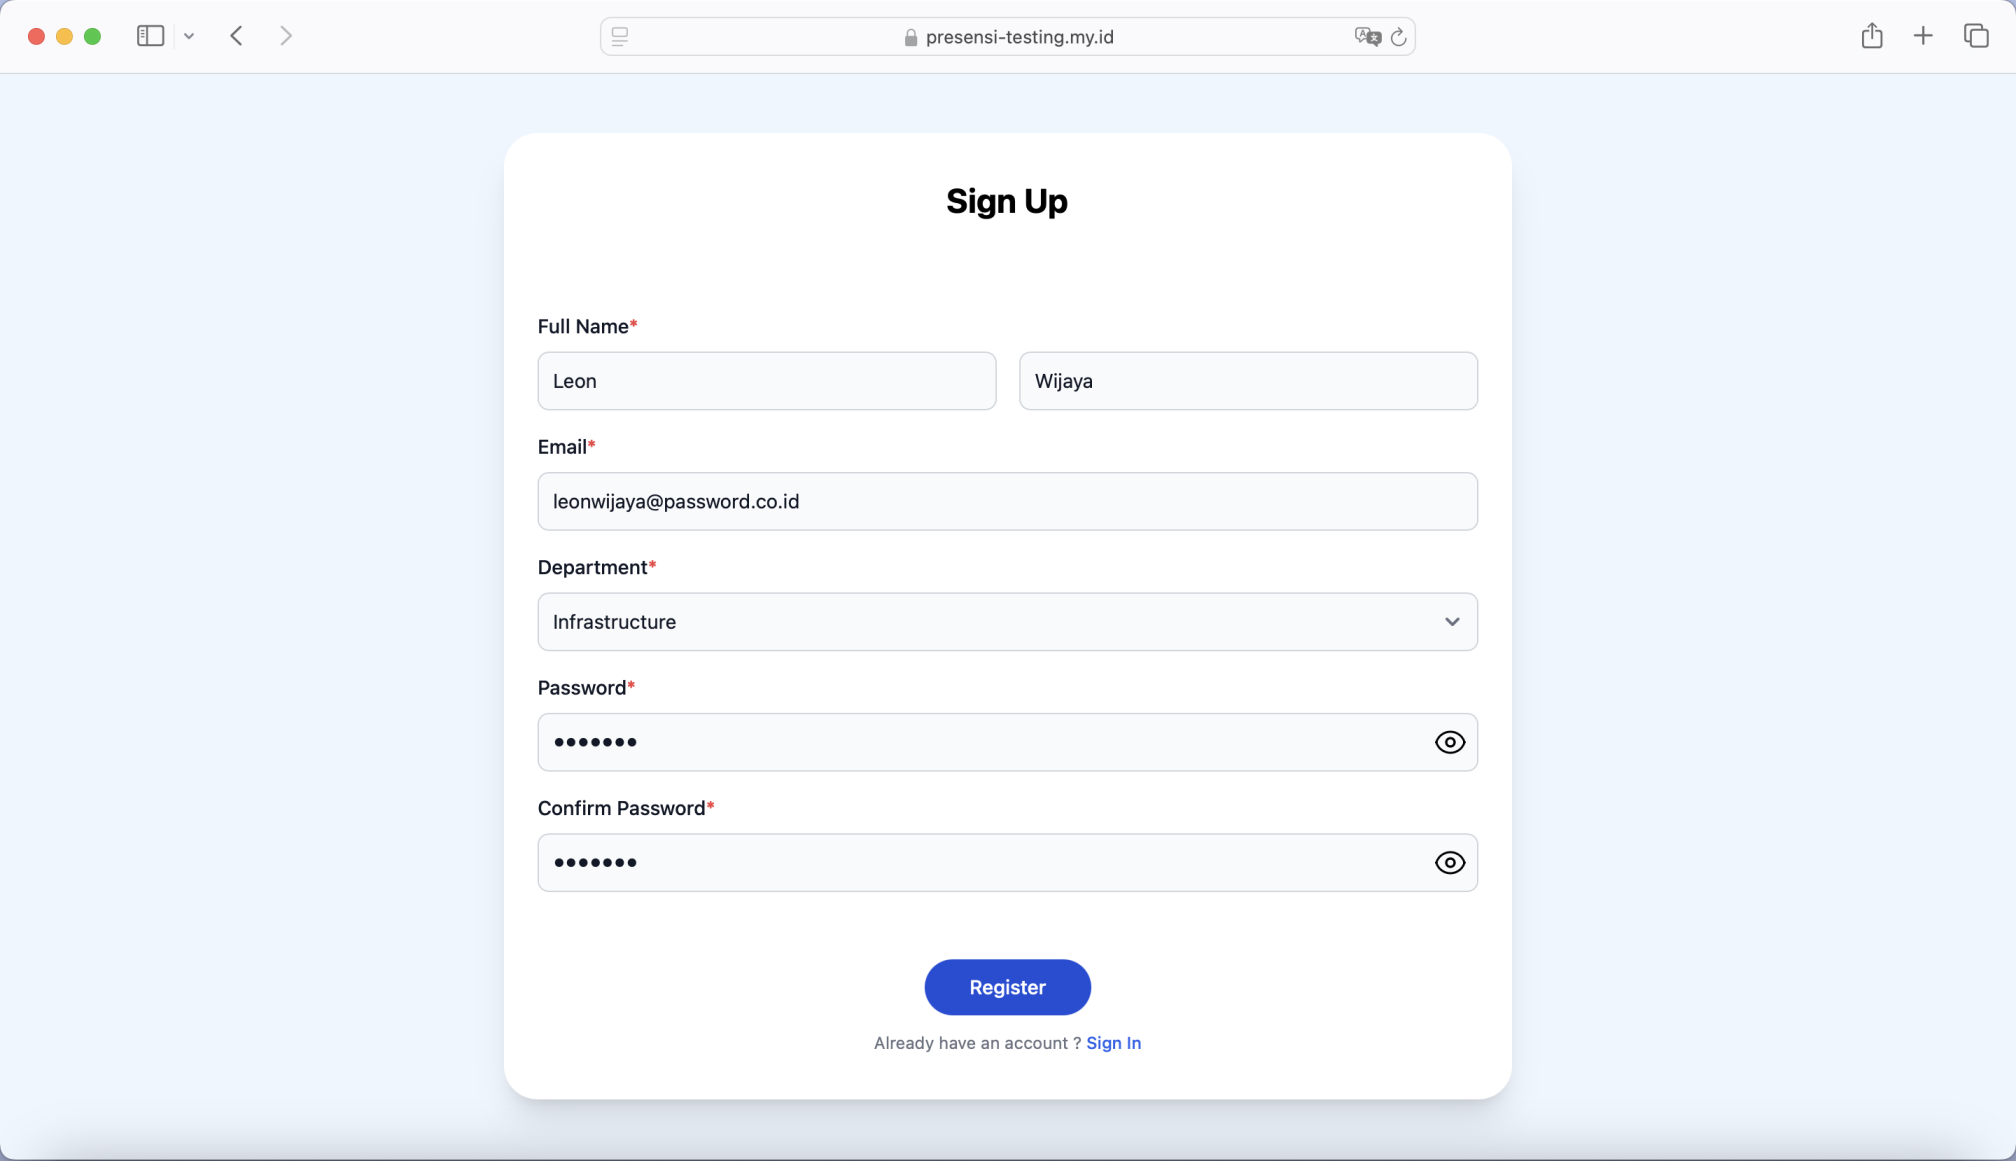
\includegraphics[width=10cm]{Gambar/bab3/user-manual/user-manual-halaman-sign-up.png}
    	\caption{Halaman Registrasi Akun}
    	\label{fig:user-manual-halaman-sign-up}
        \end{figure}
        \FloatBarrier

        \begin{figure}[!htbp]
    	\centering
    	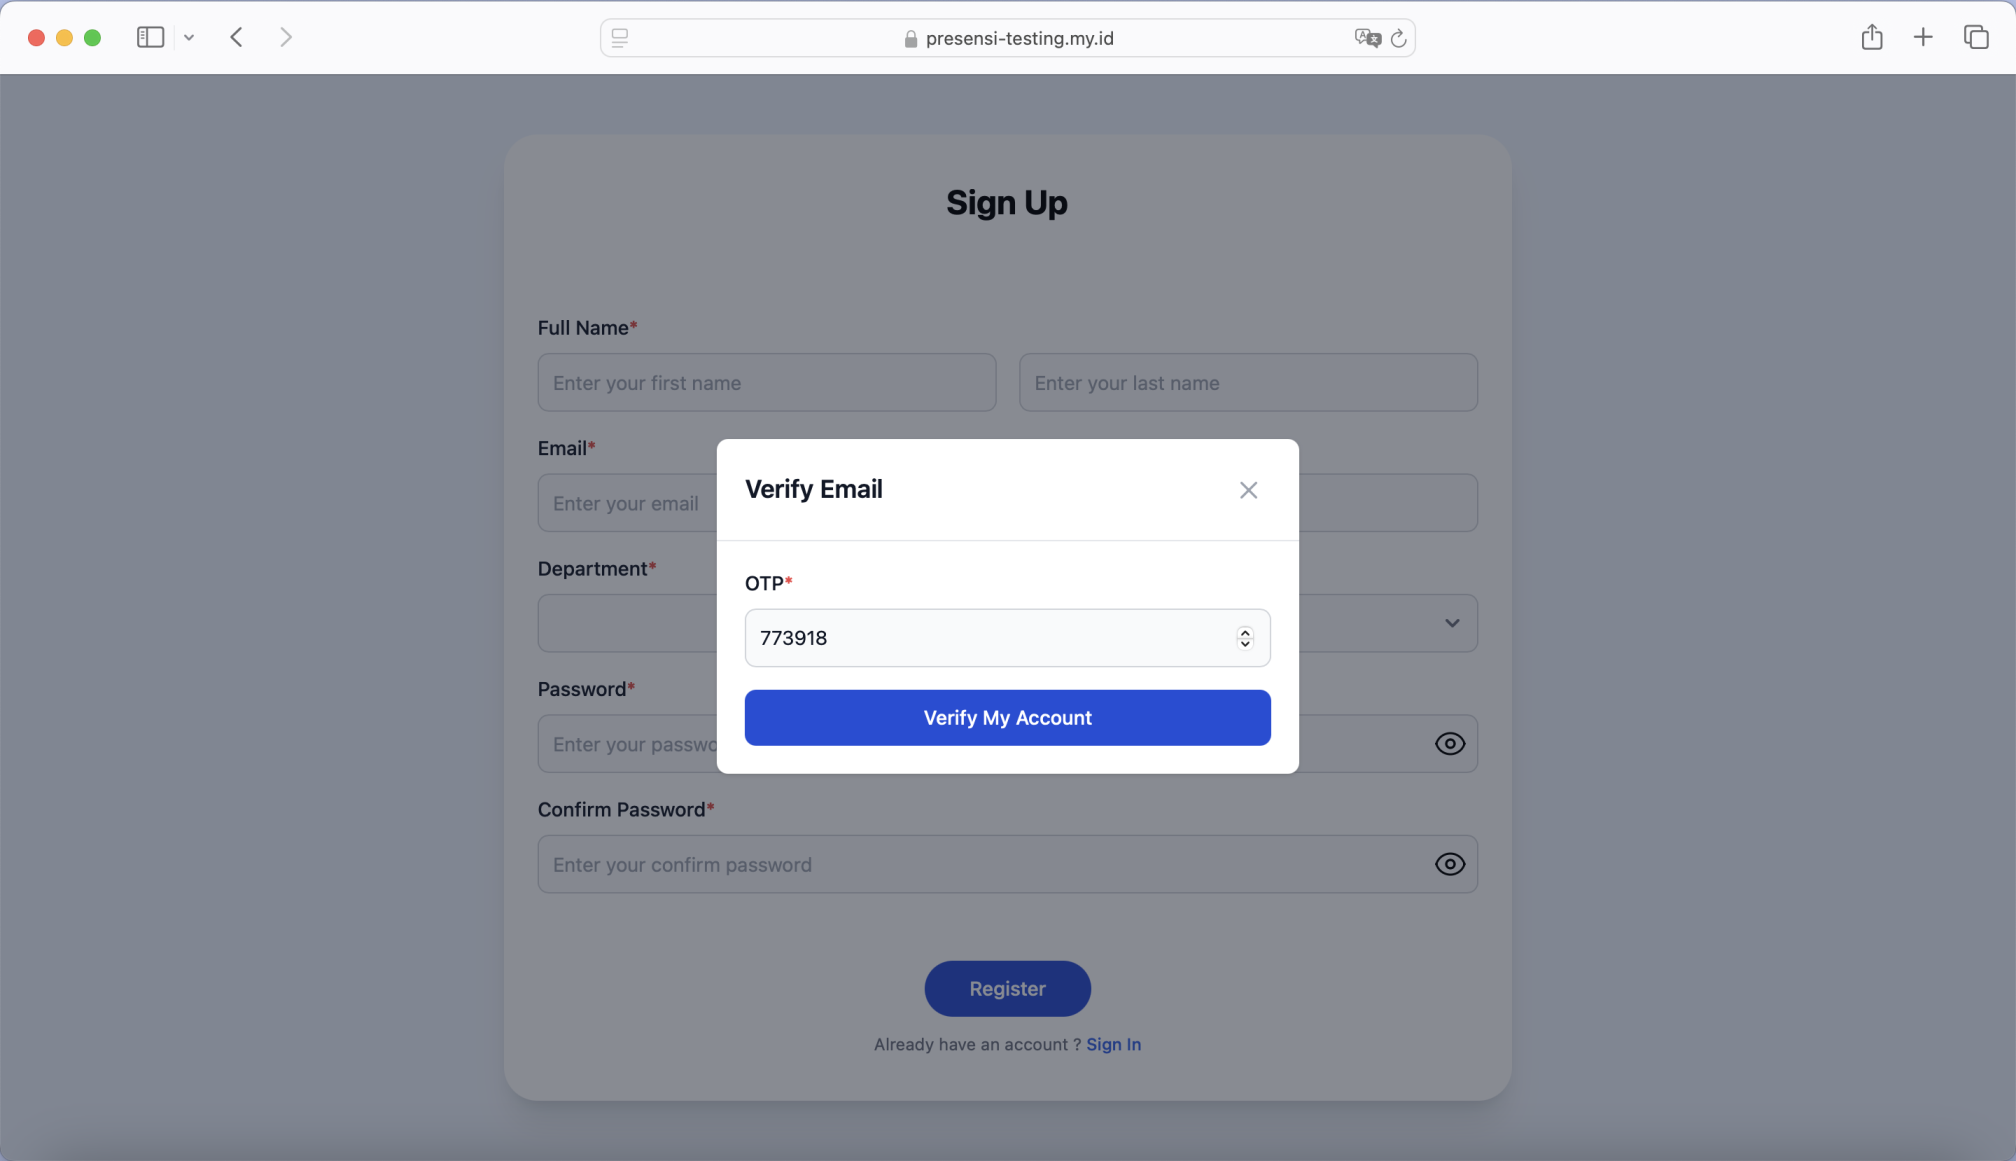
\includegraphics[width=10cm]{Gambar/bab3/user-manual/user-manual-verifikasi-email.png}
    	\caption{Modal Verifikasi \textit{Email}}
    	\label{fig:user-manual-verifikasi-email}
        \end{figure}
        \FloatBarrier

        \begin{figure}[!htbp]
    	\centering
    	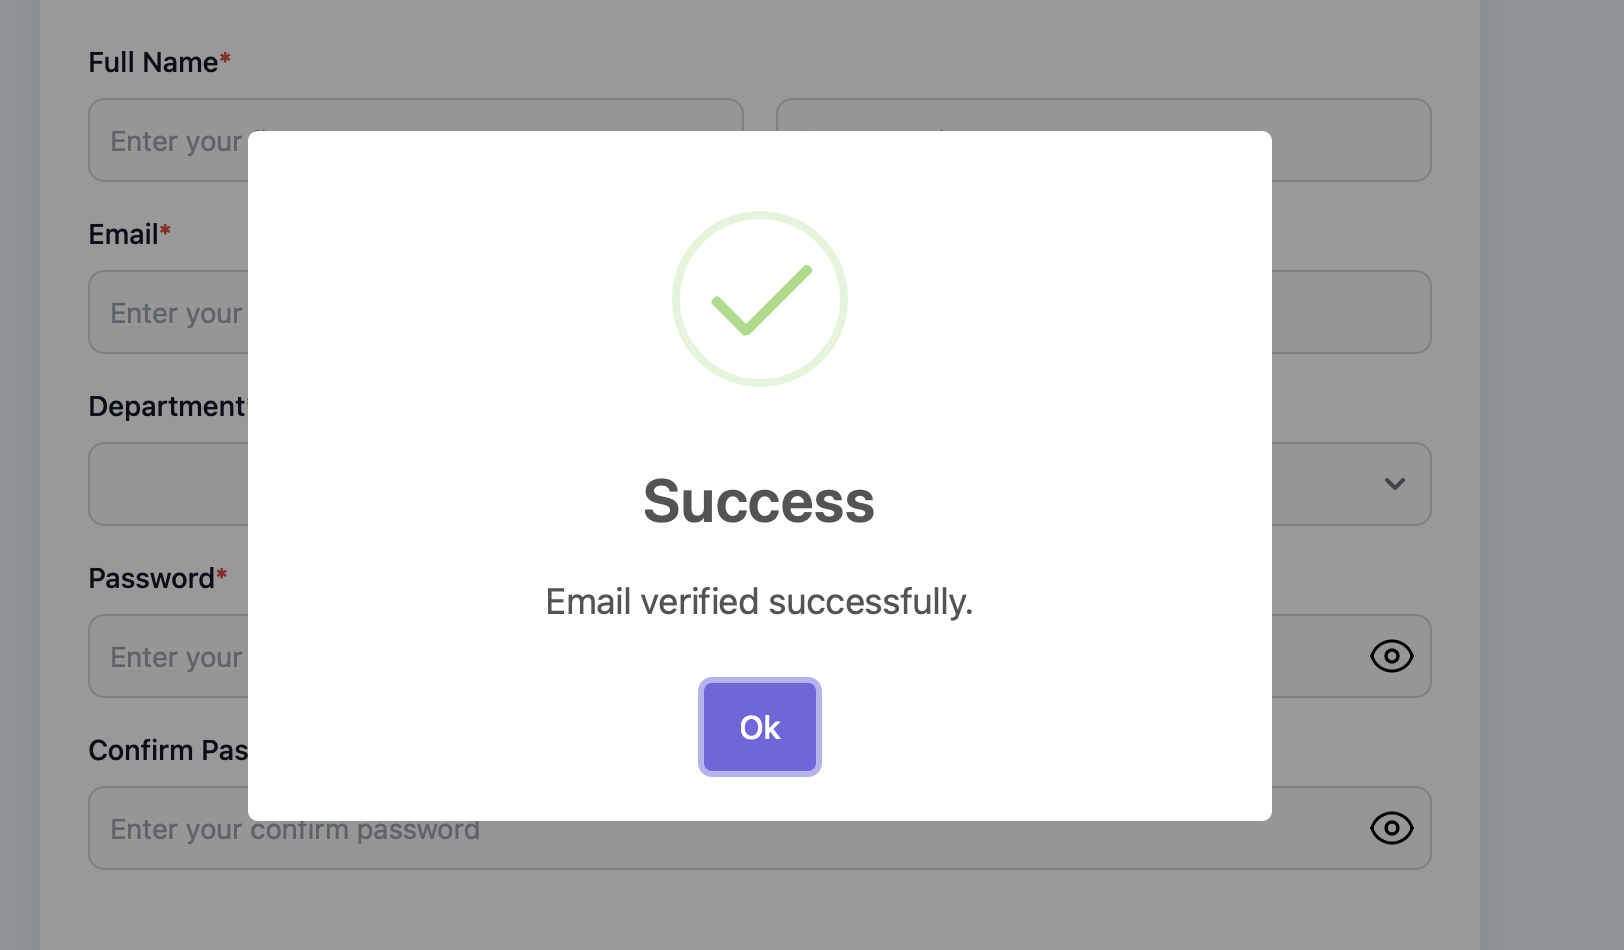
\includegraphics[width=10cm]{Gambar/bab3/user-manual/user-manual-berhasil-verifikasi.png}
    	\caption{Pesan Berhasil Verifikasi \textit{Email}}
    	\label{fig:user-manual-pesan-berhasil-verifikasi}
        \end{figure}
        \FloatBarrier
    \end{enumerate}

    \item Melihat Jadwal Kerja
    \begin{enumerate}
        \item Melakukan \textit{login} pada aplikasi presensi \textit{online} yang terdapat pada \textbf{Manual \ref{item:melakukan-login}}.
        \item Menekan tombol "\textit{Presence}" pada \textit{navigation bar} yang terletak di paling atas. \textbf{\ref{fig:user-manual-tombol-presence-pada-navigation-bar}} menunjukkan tombol \textit{"Presence"} pada \textit{navigation bar}.
        \item Pada halaman \textit{presence}, tekan tombol \textit{"Check Schedule"} yang terletak ditengah halaman. \textbf{\ref{fig:user-manual-tombol-check-schedule}} menunjukkan tombol \textit{"Check Schedule"} yang terletak di tengah halaman \textit{presence}.
        \item Tampilan modal informasi jadwal kerja akan muncul. \textbf{\ref{fig:user-manual-modal-check-schedule}} menunjukkan tampilan modal \textit{check schedule}.
        \begin{figure}[!htbp]
    	\centering
    	
\includegraphics[width=8cm]{Gambar/bab3/user-manual/user-manual-navbar-presence.png}
    	\caption{Tombol \textit{Presence} Pada \textit{Navigation Bar}}
    	\label{fig:user-manual-tombol-presence-pada-navigation-bar}
        \end{figure}
        \FloatBarrier
        \begin{figure}[!htbp]
    	\centering
    	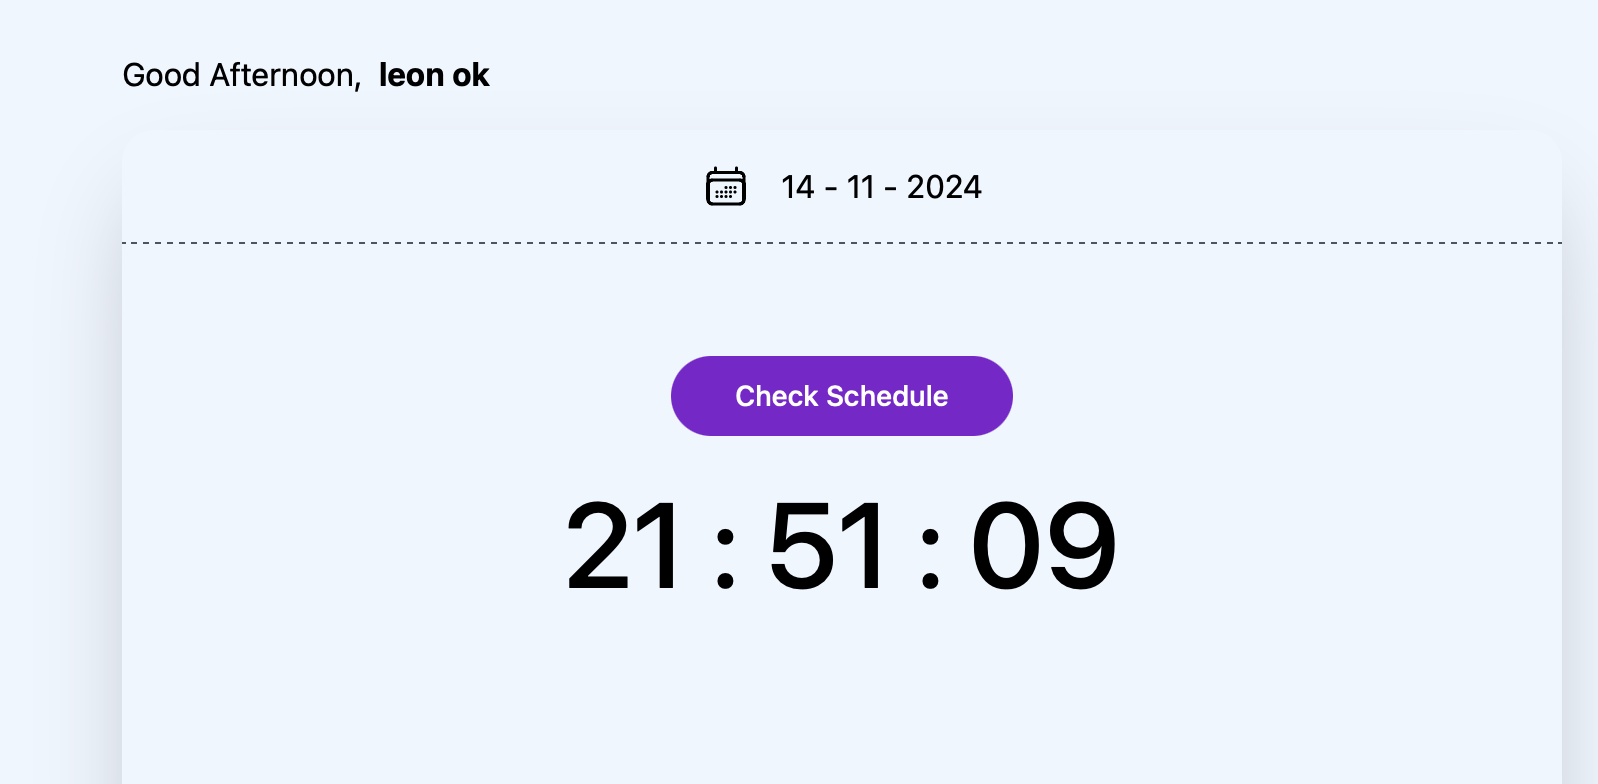
\includegraphics[width=8cm]{Gambar/bab3/user-manual/user-manual-tombol-check-schedule.png}
    	\caption{Tombol \textit{Check Schedule} Pada Halaman \textit{Presence}}
    	\label{fig:user-manual-tombol-check-schedule}
        \end{figure}
        \FloatBarrier
        \begin{figure}[!htbp]
    	\centering
    	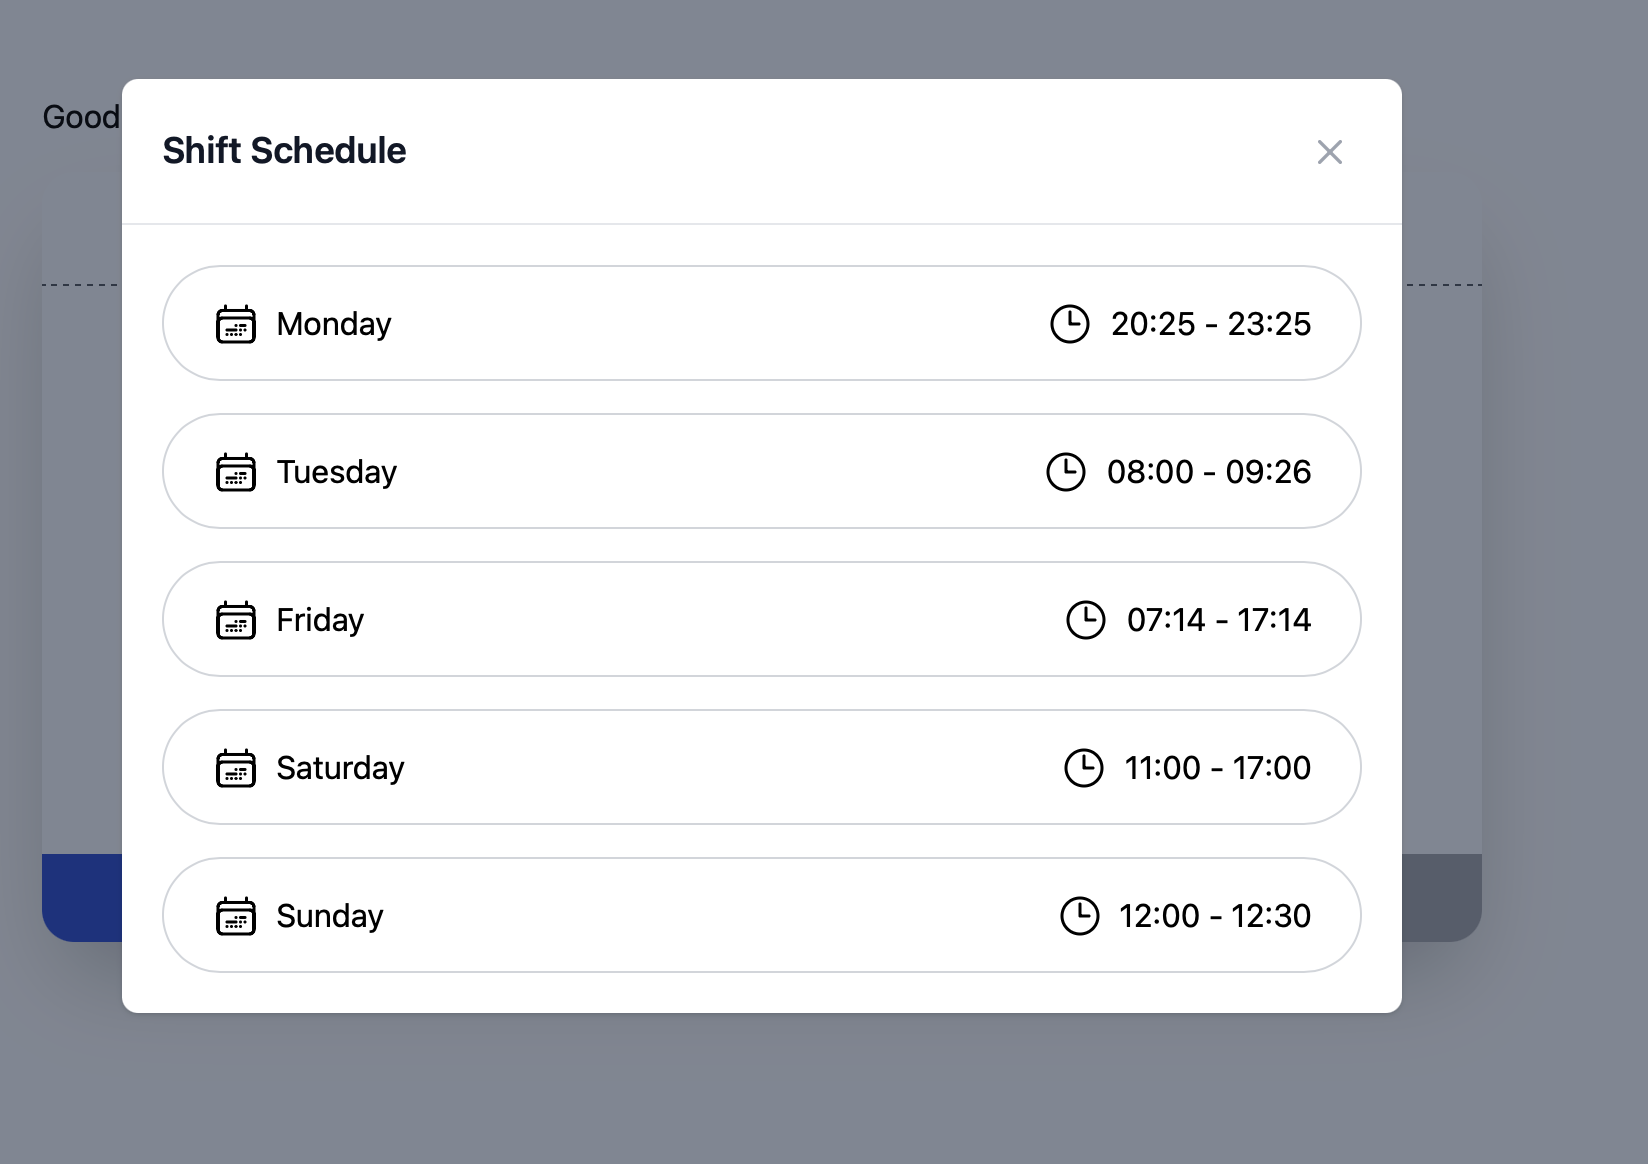
\includegraphics[width=8cm]{Gambar/bab3/user-manual/user-manual-modal-check-schedule.png}
    	\caption{Tampilan Modal \textit{Check Schedule}}
    	\label{fig:user-manual-modal-check-schedule}
        \end{figure}
        \FloatBarrier
    \end{enumerate}

    \item Melakukan \textit{Clock In}
    \begin{enumerate}
        \item Melakukan \textit{login} pada aplikasi presensi \textit{online} yang terdapat pada \textbf{Manual \ref{item:melakukan-login}}.
        \item Menekan tombol "\textit{Presence}" pada \textit{navigation bar} yang terletak di paling atas. \textbf{\ref{fig:user-manual-tombol-presence-pada-navigation-bar}} menunjukkan tombol \textit{"Presence"} pada \textit{navigation bar}.
        \item Pada halaman \textit{presence}, tekan tombol \textit{"Clock In"} yang berada ditengah halaman dan izinkan perangkat untuk mengakses lokasi. \textbf{\ref{fig:user-manual-tombol-clock-in}} menunjukkan tombol "\textit{Clock In}" pada halaman \textit{presence}.
        \begin{figure}[!htbp]
    	\centering
    	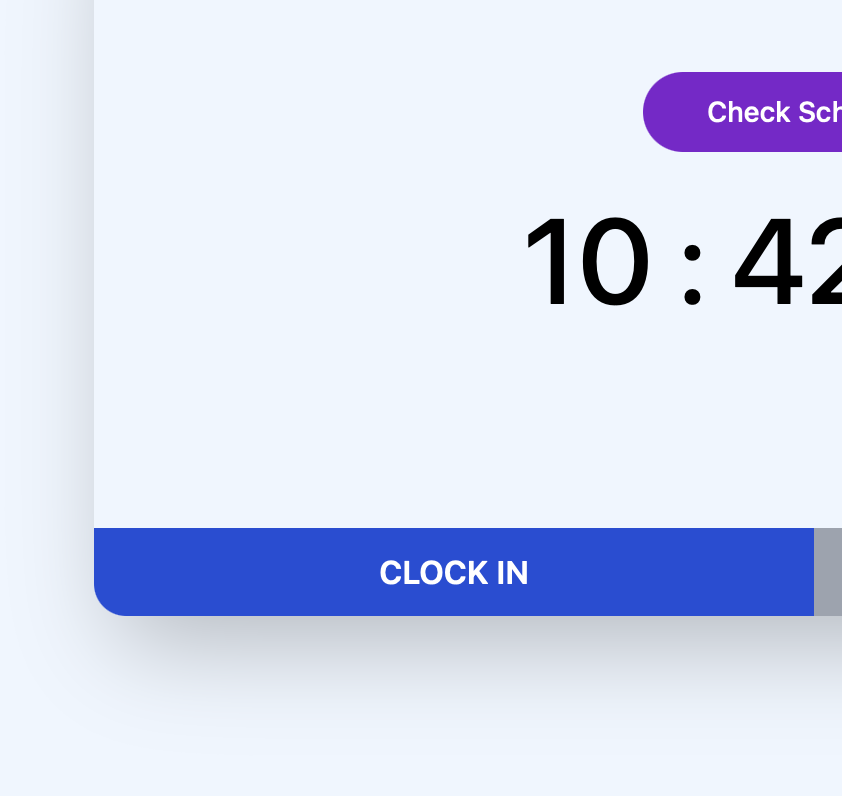
\includegraphics[width=8cm]{Gambar/bab3/user-manual/user-manual-tombol-clock-in.png}
    	\caption{Tombol \textit{Clock In} Pada Halaman \textit{Presence}}
    	\label{fig:user-manual-tombol-clock-in}
        \end{figure}
        \FloatBarrier
        \item Mengisi seluruh \textit{input form} pada modal \textit{clock in}. \textbf{\ref{fig:user-manual-modal-clock-in}} menunjukkan tampilan modal \textit{clock in}.
        \begin{figure}[!htbp]
    	\centering
    	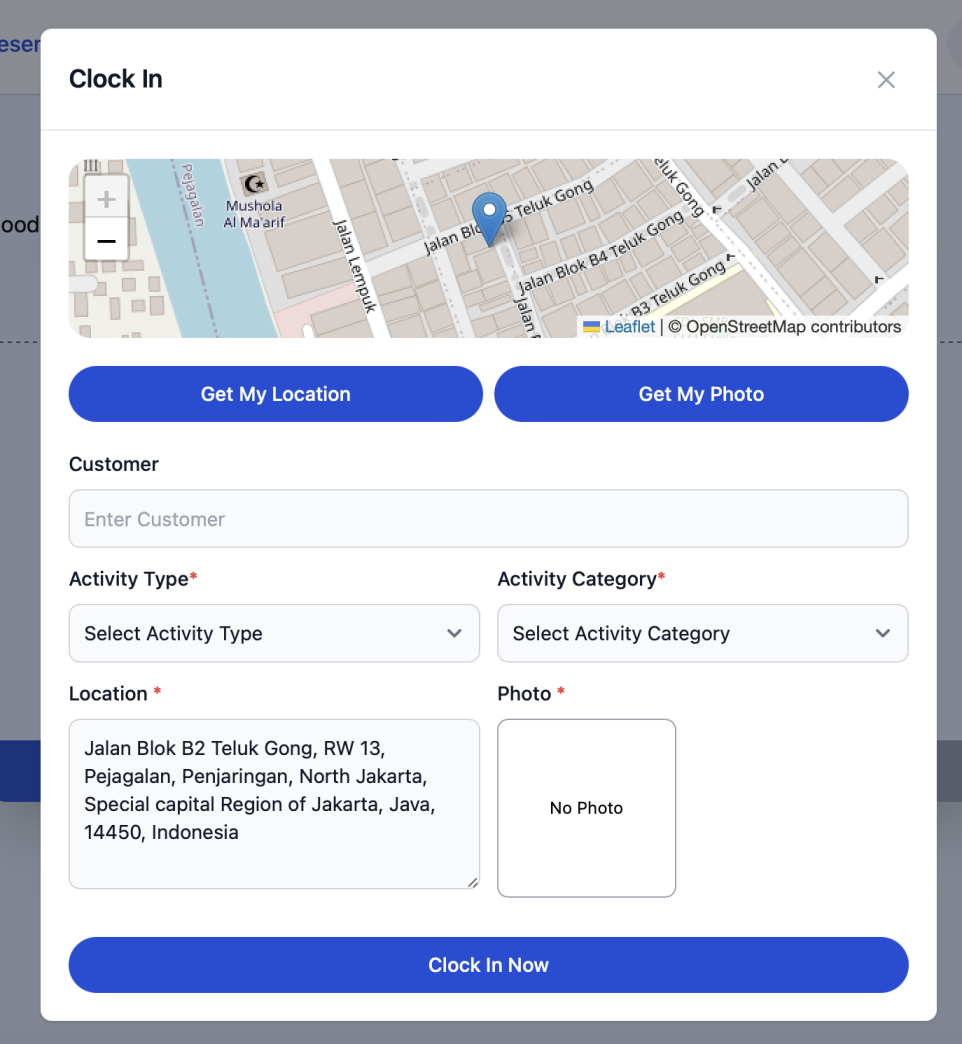
\includegraphics[width=5cm]{Gambar/bab3/user-manual/user-manual-modal-clock-in.png}
    	\caption{Modal \textit{Clock In}}
    	\label{fig:user-manual-modal-clock-in}
        \end{figure}
        \FloatBarrier
        \item Menekan tombol "\textit{Get My Photo}" pada modal \textit{clock in} untuk mengambil foto presensi dan izinkan perangkat untuk mengakses kamera. \textbf{\ref{fig:user-manual-tombol-get-my-photo-pada-modal-clock-in}} menunjukkan tombol "\textit{Get My Photo}" pada modal \textit{clock in}.
        \begin{figure}[!htbp]
    	\centering
    	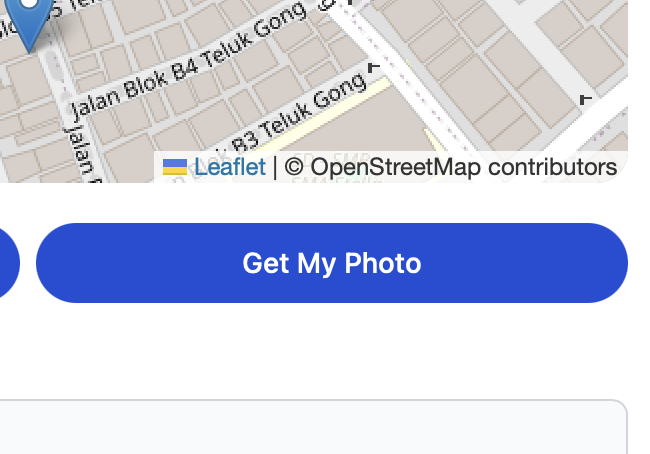
\includegraphics[width=8cm]{Gambar/bab3/user-manual/user-manual-tombol-get-my-photo-clock-in.png}
    	\caption{Tombol \textit{Get My Photo} Pada Modal \textit{Clock In}}
    	\label{fig:user-manual-tombol-get-my-photo-pada-modal-clock-in}
        \end{figure}
        \FloatBarrier

        \item Mengambil foto wajah pada modal kamera, pastikan posisi kepala berada ditengah lingkaran yang telah ditentukan pada kamera dan tekan tombol bulat untuk mengambil foto. \textbf{\ref{fig:user-manual-modal-kamera-clock-in}} menunjukkan tampilan modal kamera saat \textit{clock in}.
        \begin{figure}[!htbp]
    	\centering
    	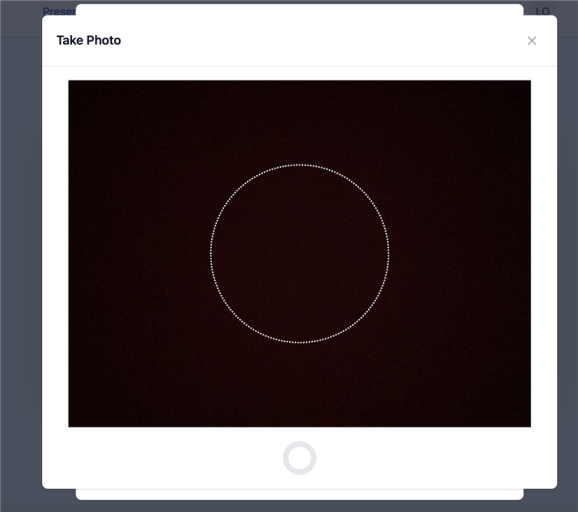
\includegraphics[width=8cm]{Gambar/bab3/user-manual/user-manual-modal-kamera-clock-in.png}
    	\caption{Modal Kamera \textit{Clock In}}
    	\label{fig:user-manual-modal-kamera-clock-in}
        \end{figure}
        \FloatBarrier
        \item Saat berhasil ambil foto, maka modal kamera akan tertutup dan membuka modal \textit{clock in} kembali. Tekan tombol \textit{"Clock In Now"} untuk menyimpan presensi masuk. \textbf{\ref{fig:user-manual-tombol-clock-in-now-pada-modal-clock-in}} menunjukkan tombol "\textit{Clock In Now}" pada modal \textit{clock in}.
        \begin{figure}[!htbp]
    	\centering
    	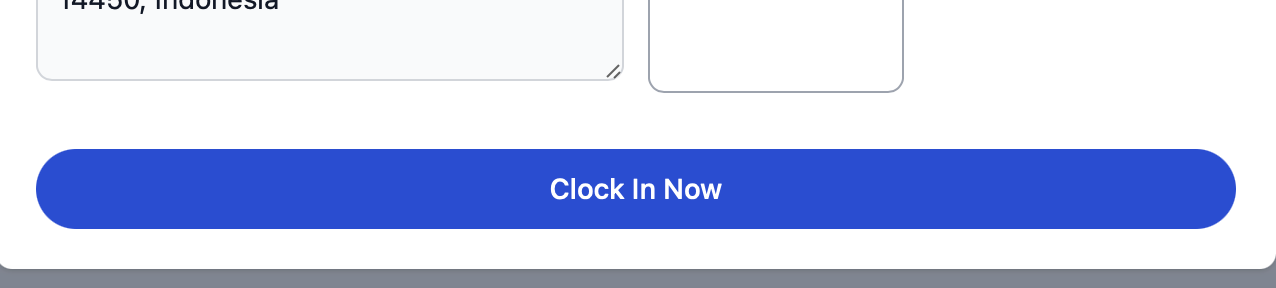
\includegraphics[width=8cm]{Gambar/bab3/user-manual/user-manual-tombol-clock-in-now.png}
    	\caption{Tombol \textit{Clock In Now} Pada Modal \textit{Clock In}}
    	\label{fig:user-manual-tombol-clock-in-now-pada-modal-clock-in}
        \end{figure}
        \FloatBarrier
    \end{enumerate}

    \item Melakukan \textit{Clock Out}
    \begin{enumerate}
        \item Melakukan \textit{login} pada aplikasi presensi \textit{online} yang terdapat pada \textbf{Manual \ref{item:melakukan-login}}.
        \item Menekan tombol "\textit{Presence}" pada \textit{navigation bar} yang terletak di paling atas. \textbf{\ref{fig:user-manual-tombol-presence-pada-navigation-bar}} menunjukkan tombol \textit{"Presence"} pada \textit{navigation bar}.
        \item Pastikan sudah melakukan \textit{clock in} sebelumya, pada halaman \textit{presence}, tekan tombol \textit{"Clock Out"} yang berada ditengah halaman dan izinkan perangkat untuk mengakses lokasi. \textbf{\ref{fig:user-manual-tombol-clock-out}} menunjukkan tombol "\textit{Clock Out}" pada halaman \textit{presence}.
        \begin{figure}[!htbp]
    	\centering
    	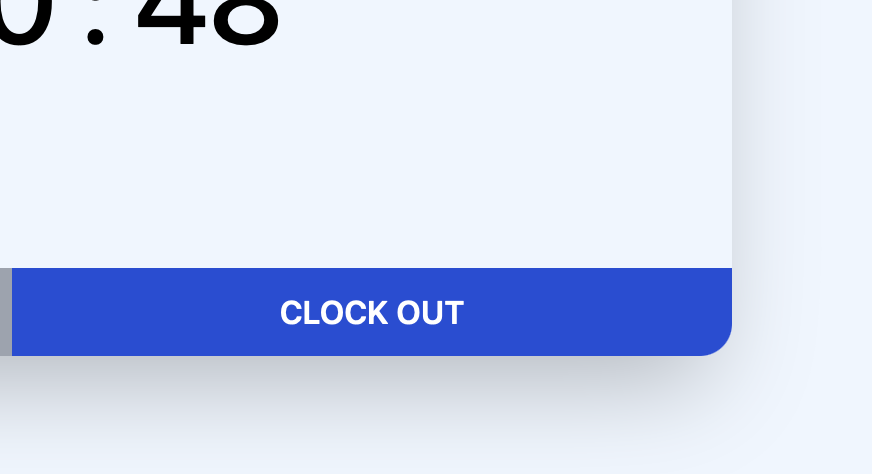
\includegraphics[width=8cm]{Gambar/bab3/user-manual/user-manual-tombol-clock-out.png}
    	\caption{Tombol \textit{Clock Out} Pada Halaman \textit{Presence}}
    	\label{fig:user-manual-tombol-clock-out}
        \end{figure}
        \FloatBarrier
        \item Seluruh \textit{input form} pada modal \textit{clock out} dapat dilakukan perubahan. \textbf{\ref{fig:user-manual-modal-clock-out}} menunjukkan tampilan modal \textit{clock out}.
        \begin{figure}[!htbp]
    	\centering
    	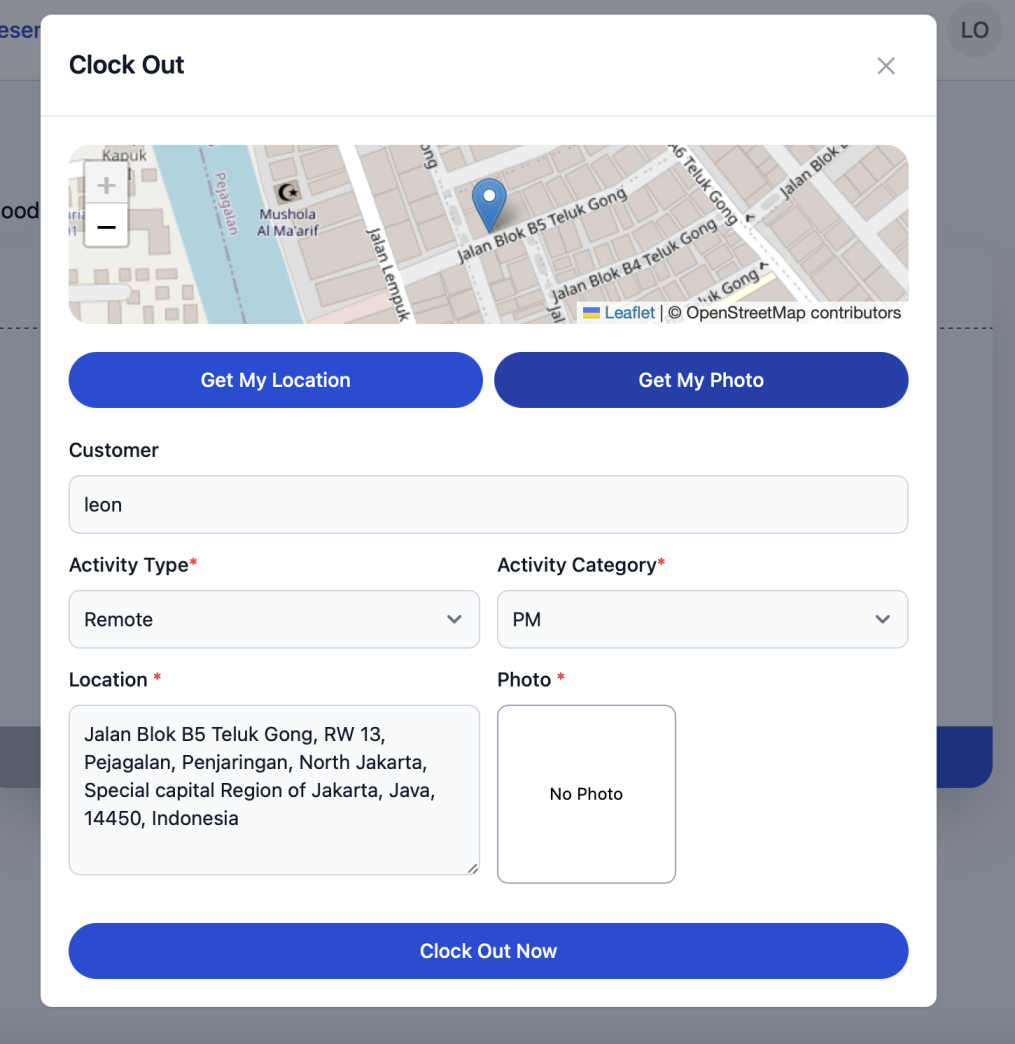
\includegraphics[width=5cm]{Gambar/bab3/user-manual/user-manual-modal-clock-out.png}
    	\caption{Modal \textit{Clock Out}}
    	\label{fig:user-manual-modal-clock-out}
        \end{figure}
        \FloatBarrier
        \item Menekan tombol "\textit{Get My Photo}" pada modal \textit{clock out} untuk mengambil foto presensi dan izinkan perangkat untuk mengakses kamera. \textbf{\ref{fig:user-manual-tombol-get-my-photo-pada-modal-clock-out}} menunjukkan tombol "\textit{Get My Photo}" pada modal \textit{clock out}.
        \begin{figure}[!htbp]
    	\centering
    	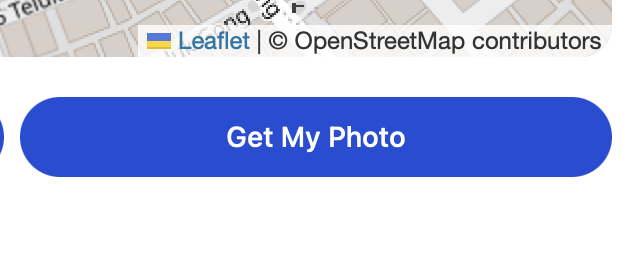
\includegraphics[width=8cm]{Gambar/bab3/user-manual/user-manual-get-my-photo-clock-out.png}
    	\caption{Tombol \textit{Get My Photo} Pada Modal \textit{Clock Out}}
    	\label{fig:user-manual-tombol-get-my-photo-pada-modal-clock-out}
        \end{figure}
        \FloatBarrier

        \item Mengambil foto wajah pada modal kamera, pastikan posisi kepala berada ditengah lingkaran yang telah ditentukan pada kamera dan tekan tombol bulat untuk mengambil foto. \textbf{\ref{fig:user-manual-modal-kamera-clock-out}} menunjukkan tampilan modal kamera saat \textit{clock out}.
        \begin{figure}[!htbp]
    	\centering
    	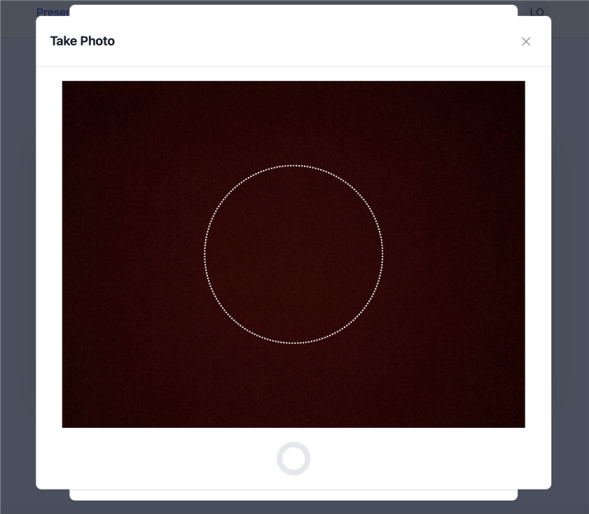
\includegraphics[width=8cm]{Gambar/bab3/user-manual/user-manual-modal-kamera-clock-out.png}
    	\caption{Modal Kamera \textit{Clock Out}}
    	\label{fig:user-manual-modal-kamera-clock-out}
        \end{figure}
        \FloatBarrier
        \item Saat berhasil ambil foto, maka modal kamera akan tertutup dan membuka modal \textit{clock out} kembali. Tekan tombol \textit{"Clock Out Now"} untuk menyimpan presensi keluar. \textbf{\ref{fig:user-manual-tombol-clock-out-now-pada-modal-clock-out}} menunjukkan tombol "\textit{Clock Out Now}" pada modal \textit{clock in}.
        \begin{figure}[!htbp]
    	\centering
    	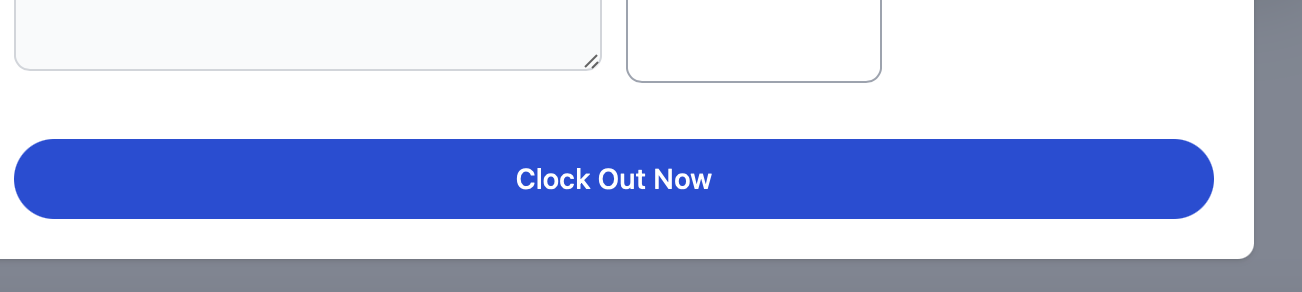
\includegraphics[width=8cm]{Gambar/bab3/user-manual/user-manual-tombol-clock-out-now.png}
    	\caption{Tombol \textit{Clock Out Now} Pada Modal \textit{Clock Out}}
    	\label{fig:user-manual-tombol-clock-out-now-pada-modal-clock-out}
        \end{figure}
        \FloatBarrier
    \end{enumerate}

    \item Melakukan Pengajuan Lembur Manual
    \begin{enumerate}
        \item Melakukan \textit{login} pada aplikasi presensi \textit{online} yang terdapat pada \textbf{Manual \ref{item:melakukan-login}}.
        \item Menekan tombol "\textit{Request}" pada \textit{navigation bar} yang terletak di paling atas. \textbf{\ref{fig:user-manual-tombol-request-pada-navigation-bar}} menunjukkan tombol \textit{"Request"} pada \textit{navigation bar}.
        \begin{figure}[!htbp]
    	\centering
    	
\includegraphics[width=8cm]{Gambar/bab3/user-manual/user-manual-navbar-request.png}
    	\caption{Tombol \textit{Request} Pada \textit{Navigation Bar}}
    	\label{fig:user-manual-tombol-request-pada-navigation-bar}
        \end{figure}
        \FloatBarrier
        \item Mengisi seluruh \textit{input form} pada halaman \textit{request} dan tekan tombol \textit{"Submit"} untuk menyimpan data pengajuan lembur. \textbf{\ref{fig:user-manual-halaman-pengajuan-lembur-manual}} menunjukkan halaman pengajuan lembur manual.
        \begin{figure}[!htbp]
    	\centering
    	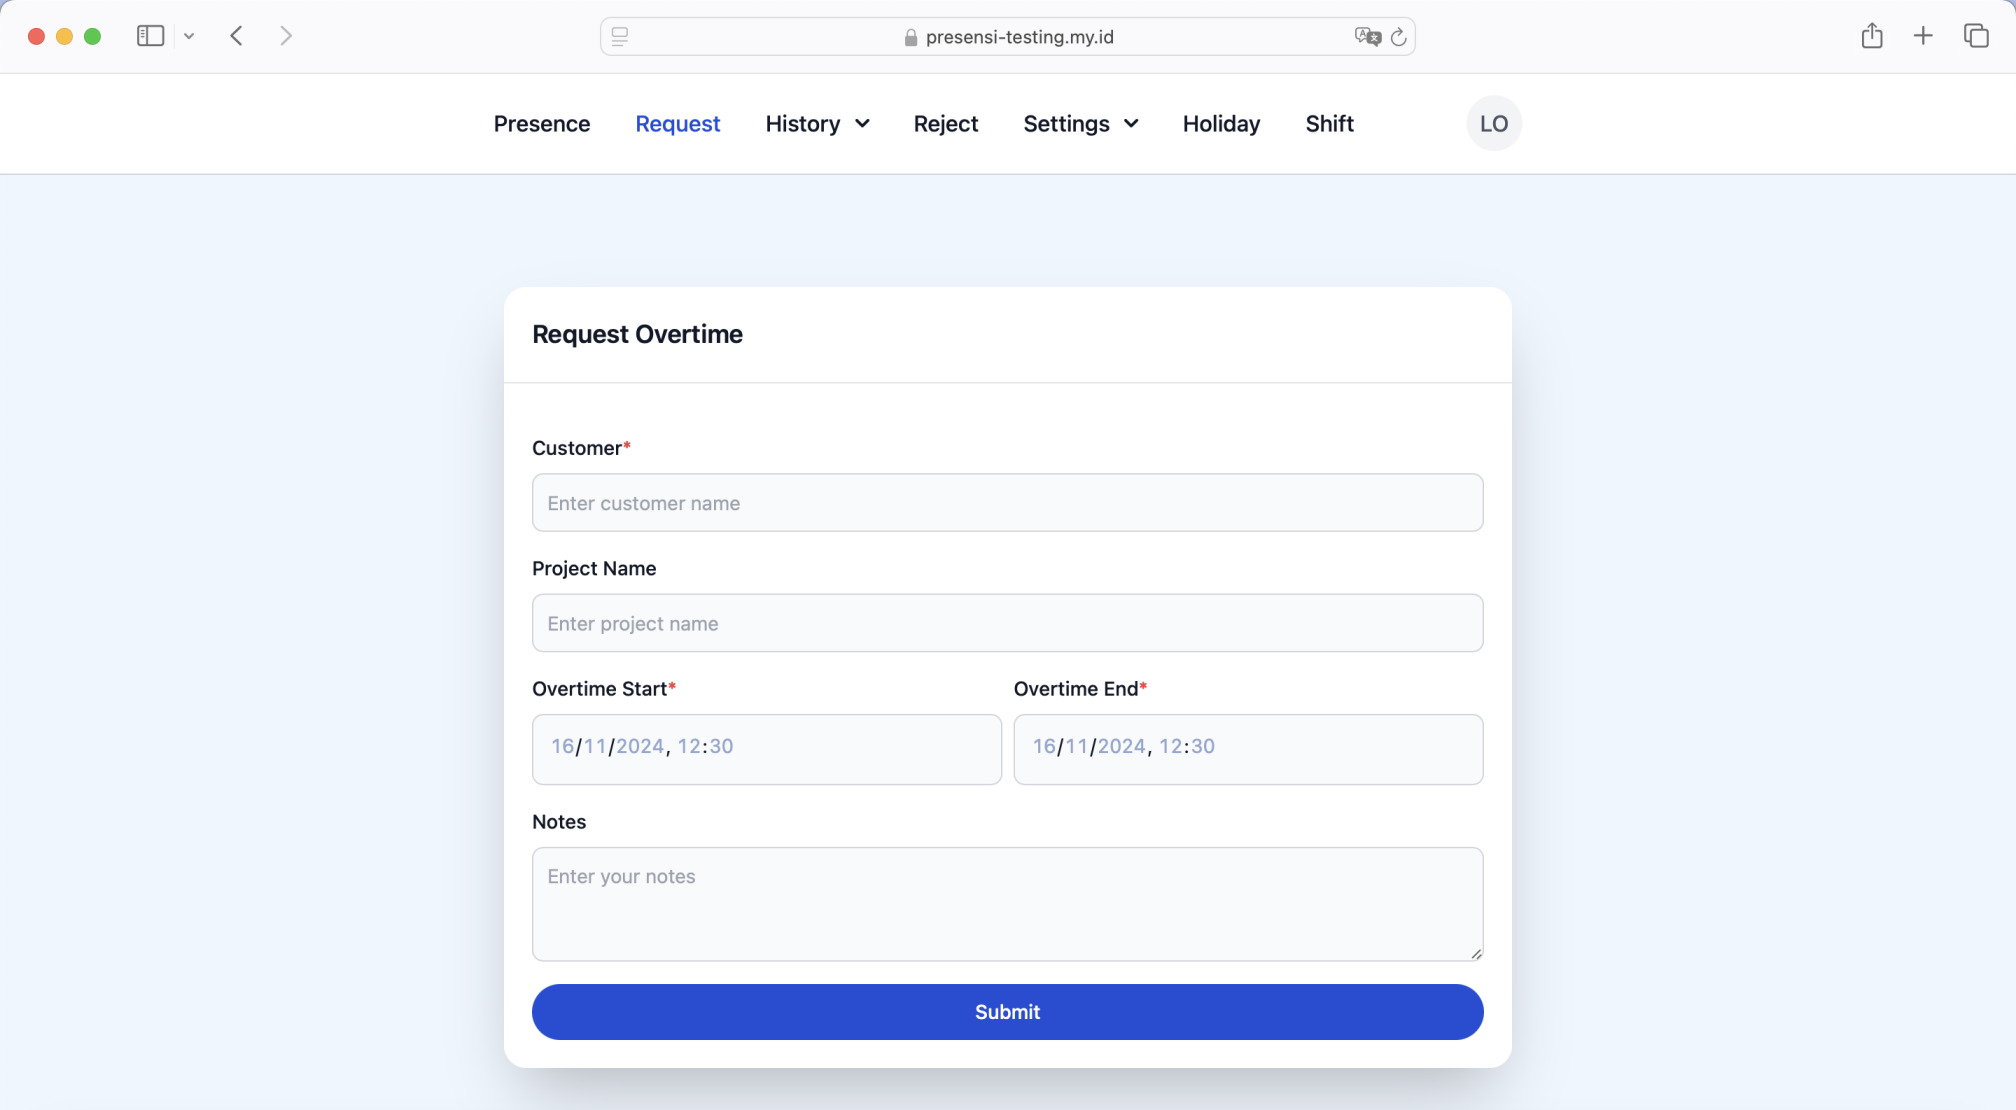
\includegraphics[width=8cm]{Gambar/bab3/user-manual/user-manual-pengajuan-lembur-manual.png}
    	\caption{Tampilan Halaman Pengajuan Lembur Manual}
    	\label{fig:user-manual-halaman-pengajuan-lembur-manual}
        \end{figure}
        \FloatBarrier
    \end{enumerate}

    \item Melihat Riwayat Presensi\label{item:melihat-riwayat-presensi}
    \begin{enumerate}
        \item Melakukan \textit{login} pada aplikasi presensi \textit{online} yang terdapat pada \textbf{Manual \ref{item:melakukan-login}}.
        \item Menekan tombol "\textit{History}" pada \textit{navigation bar} yang terletak di paling atas dan memilih tombol \textit{"Attendance History"}. \textbf{\ref{fig:user-manual-tombol-attendance-history-pada-navigation-bar}} menunjukkan tombol \textit{"Attendance History"} pada \textit{navigation bar}.
        \begin{figure}[!htbp]
    	\centering
    	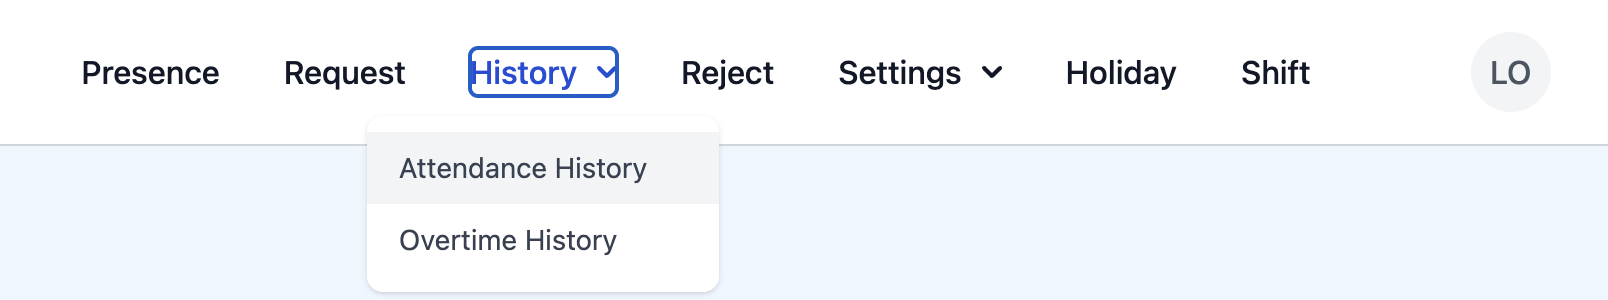
\includegraphics[width=8cm]{Gambar/bab3/user-manual/user-manual-navbar-attendance-history.png}
    	\caption{Tombol \textit{Attendance History} Pada \textit{Navigation Bar}}
    	\label{fig:user-manual-tombol-attendance-history-pada-navigation-bar}
        \end{figure}
        \FloatBarrier
        \item Seluruh daftar data riwayat presensi akan ditampilkan pada halaman \textit{attendance history}. \textbf{\ref{fig:user-manual-halaman-riwayat-presensi}} menunjukkan halaman \textit{attendance history}. 
        \begin{figure}[!htbp]
    	\centering
    	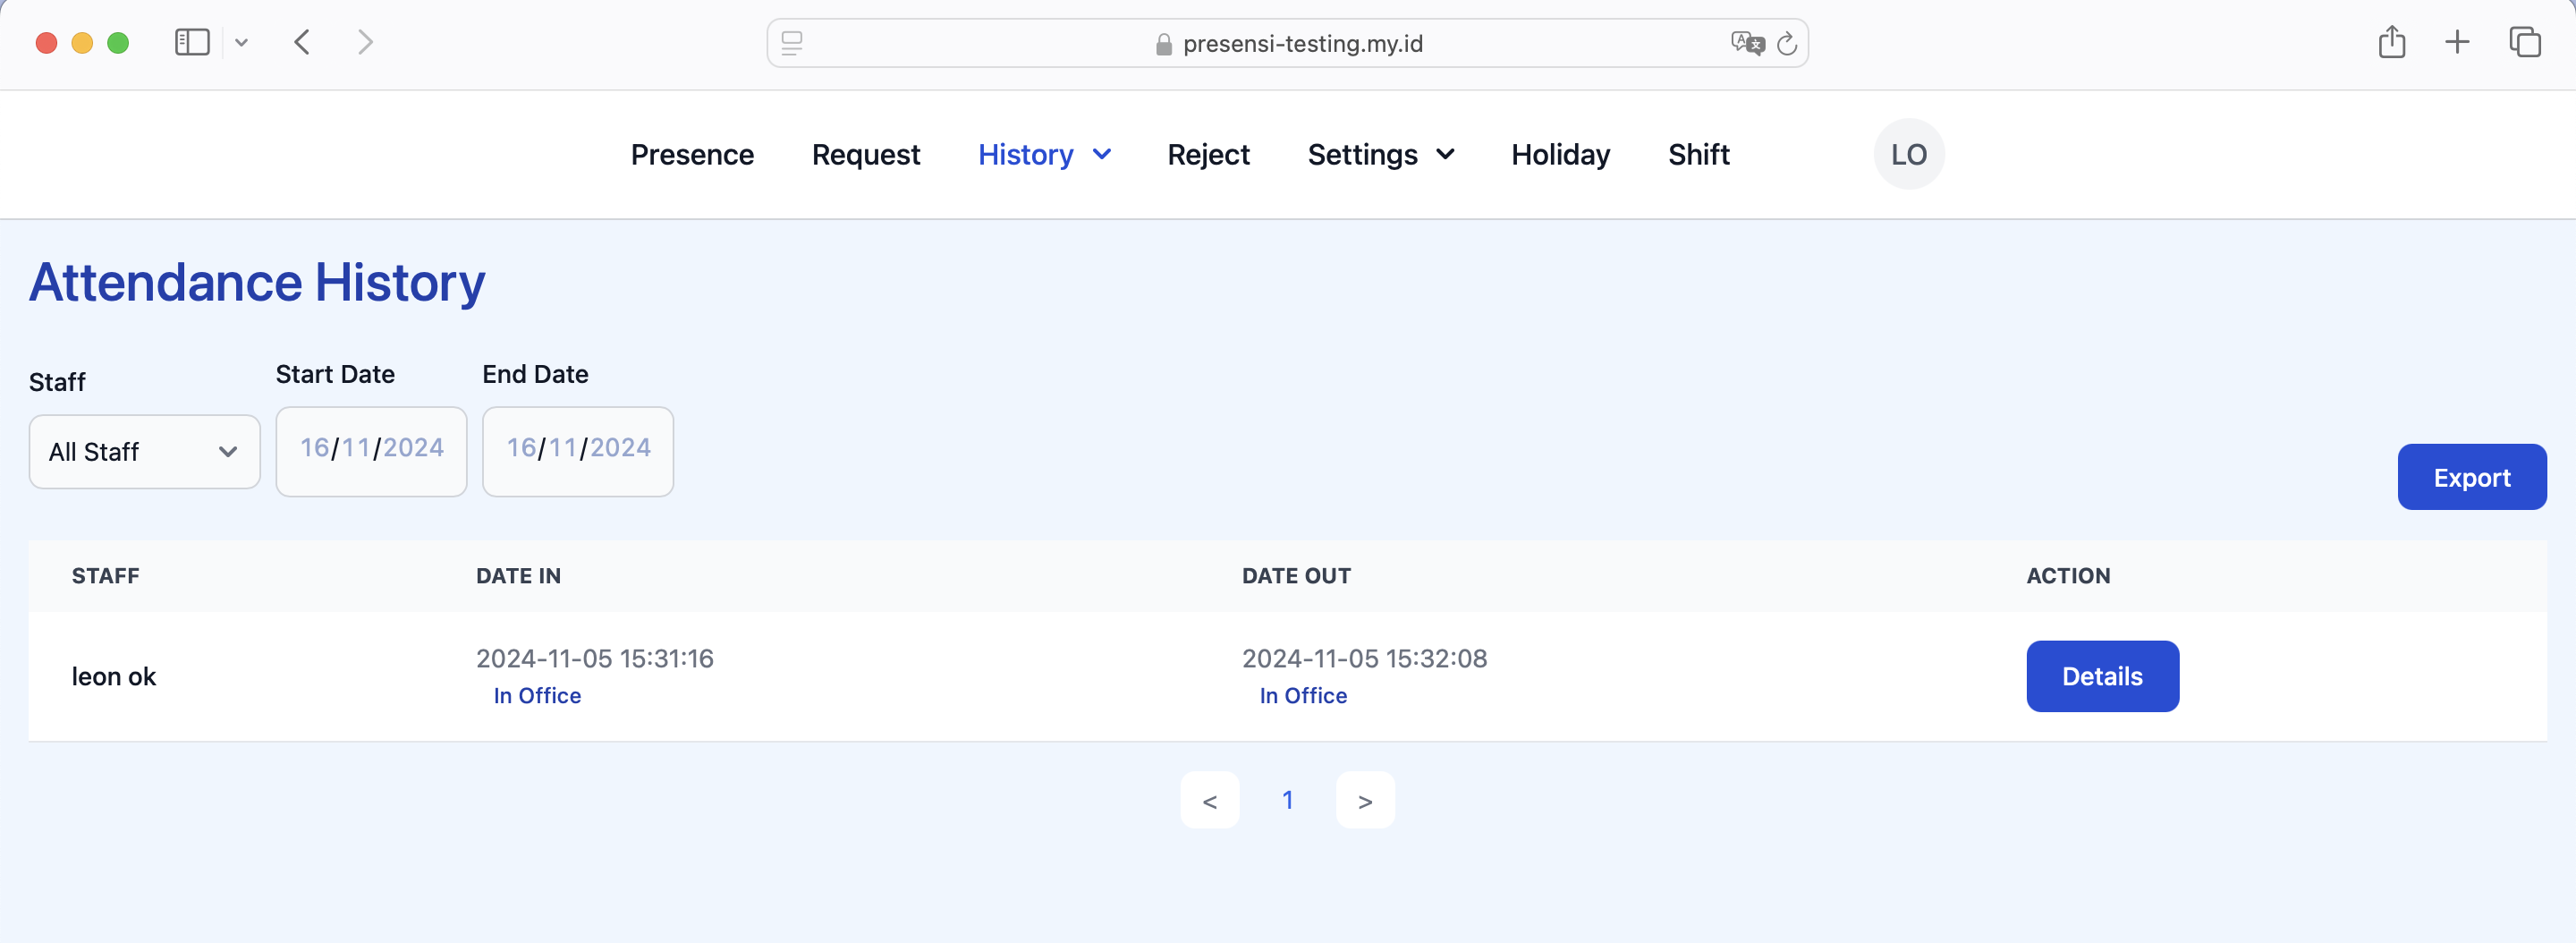
\includegraphics[width=8cm]{Gambar/bab3/user-manual/user-manual-halaman-riwayat-presensi.png}
    	\caption{Halaman \textit{Attendance History}}
    	\label{fig:user-manual-halaman-riwayat-presensi}
        \end{figure}
        \FloatBarrier
    \end{enumerate}

    \item Melihat Detail Riwayat Presensi
    \begin{enumerate}
        \item Membuka halaman riwayat presensi yang terdapat pada \textbf{Manual \ref{item:melihat-riwayat-presensi}}.
        \item Menekan tombol "\textit{Detail}" pada salah satu data presensi. Sistem akan menampilkan modal detail riwayat presensi beserta informasi lengkap riwayat presensi. \textbf{\ref{fig:user-manual-modal-attendance-history-details}} menunjukkan modal \textit{attendance history details}.
        \begin{figure}[!htbp]
    	\centering
    	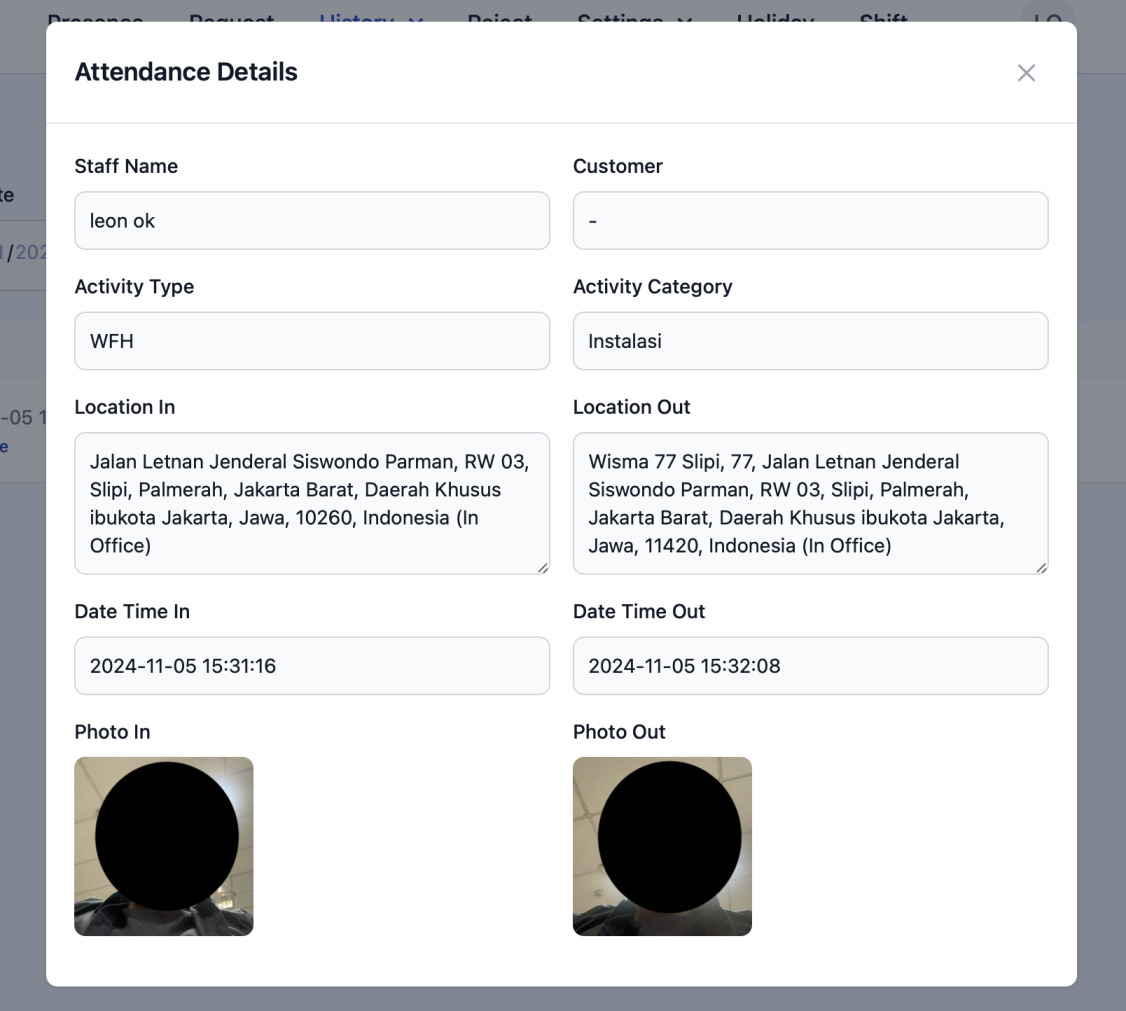
\includegraphics[width=8cm]{Gambar/bab3/user-manual/user-manual-detail-riwayat-presensi.png}
    	\caption{Modal \textit{Attendance History Details}}
    	\label{fig:user-manual-modal-attendance-history-details}
        \end{figure}
        \FloatBarrier
    \end{enumerate}

    \item Melakukan \textit{Export} Data Riwayat Presensi
    \begin{enumerate}
        \item Membuka halaman riwayat presensi yang terdapat pada \textbf{Manual \ref{item:melihat-riwayat-presensi}}.
        \item Menekan tombol \textit{"Export"} yang terdapat pada halaman riwayat presensi. \textbf{\ref{fig:user-manual-tombol-export-riwayat-presensi}} menunjukkan tombol untuk \textit{export} riwayat presensi menjadi format \textit{Excel}.
        \begin{figure}[!htbp]
    	\centering
    	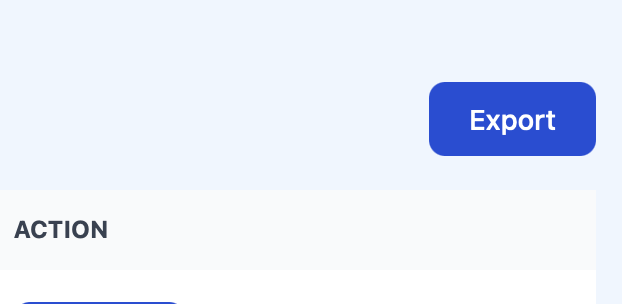
\includegraphics[width=8cm]{Gambar/bab3/user-manual/user-manual-tombol-export-riwayat-presensi.png}
    	\caption{Tombol \textit{Export} Riwayat Presensi}
    	\label{fig:user-manual-tombol-export-riwayat-presensi}
        \end{figure}
        \FloatBarrier
        \item Perangkat akan otomatis men-\textit{download file Excel} yang berisi data presensi. \textbf{\ref{fig:user-manual-file-excel-riwayat-presensi}} menunjukkan \textit{file Excel} riwayat presensi yang telah di-\textit{donwload}.
        \begin{figure}[!htbp]
    	\centering
    	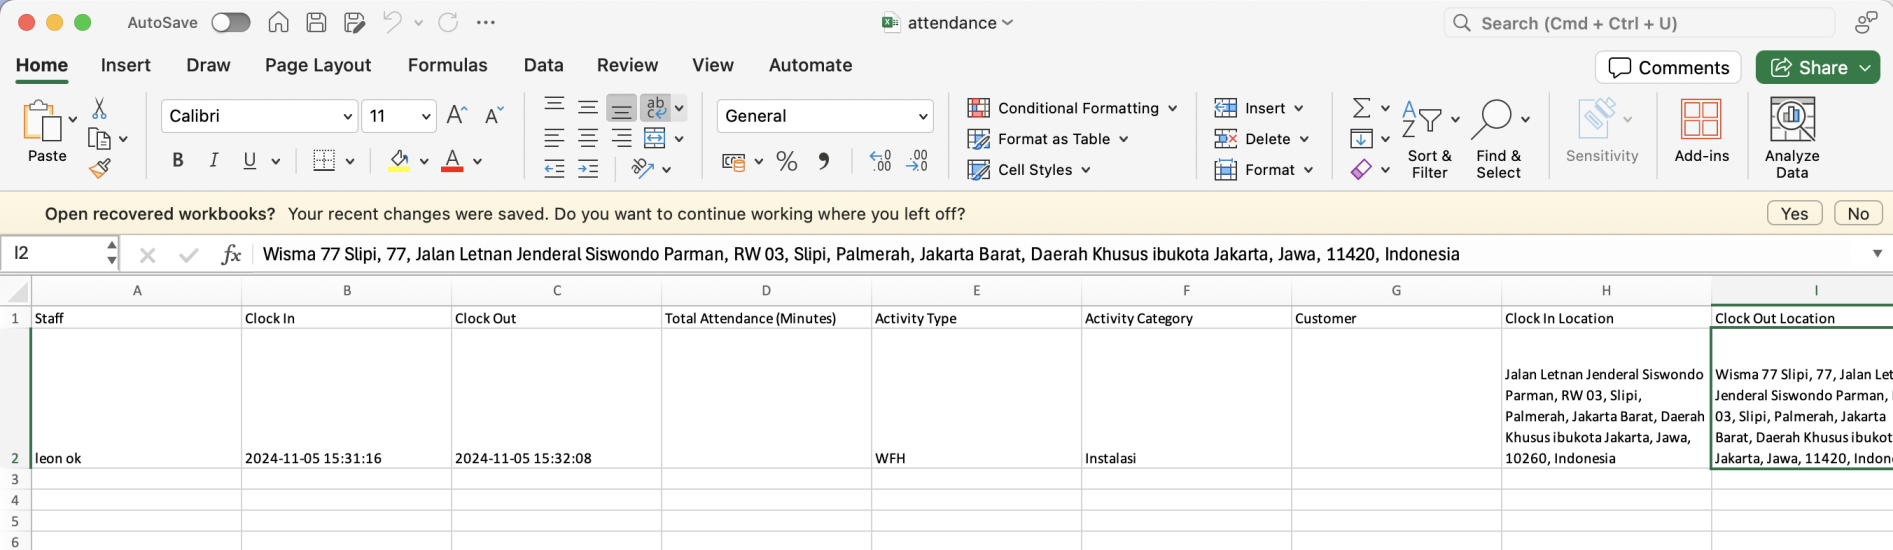
\includegraphics[width=8cm]{Gambar/bab3/user-manual/user-manual-file-excel-riwayat-presensi.png}
    	\caption{\textit{File Excel} Riwayat Presensi}
    	\label{fig:user-manual-file-excel-riwayat-presensi}
        \end{figure}
        \FloatBarrier
    \end{enumerate}

    \item Melihat Riwayat Lembur\label{item:melihat-riwayat-lembur}
    \begin{enumerate}
        \item Melakukan \textit{login} pada aplikasi presensi \textit{online} yang terdapat pada \textbf{Manual \ref{item:melakukan-login}}.
        \item Menekan tombol "\textit{History}" pada \textit{navigation bar} yang terletak di paling atas dan memilih tombol \textit{"Overtime History"}. \textbf{\ref{fig:user-manual-tombol-overtime-history-pada-navigation-bar}} menunjukkan tombol \textit{"Overtime History"} pada \textit{navigation bar}.
        \begin{figure}[!htbp]
    	\centering
    	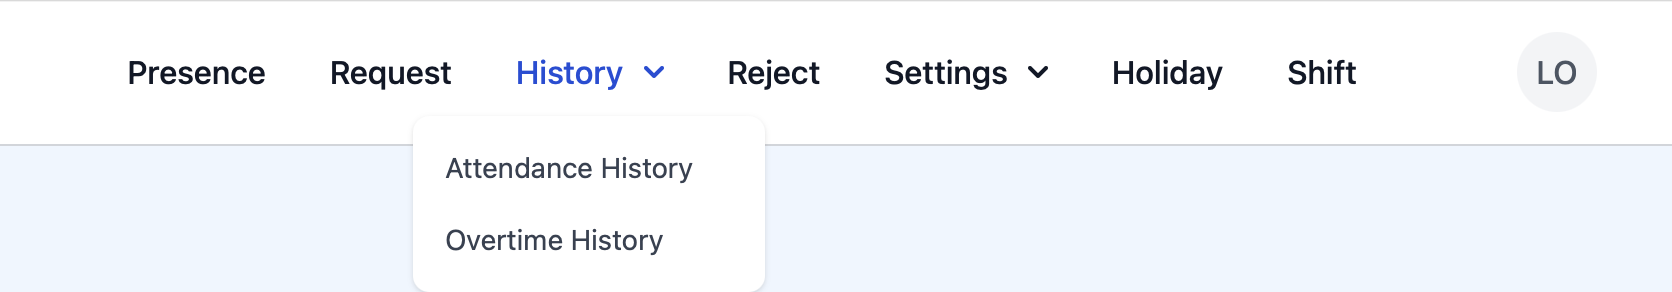
\includegraphics[width=8cm]{Gambar/bab3/user-manual/user-manual-navbar-overtime-history.png}
    	\caption{Tombol \textit{Overtime History} Pada \textit{Navigation Bar}}
    	\label{fig:user-manual-tombol-overtime-history-pada-navigation-bar}
        \end{figure}
        \FloatBarrier
        \item Seluruh daftar data riwayat lembur akan ditampilkan pada halaman \textit{overtime history}. \textbf{\ref{fig:user-manual-halaman-riwayat-lembur}} menunjukkan halaman \textit{overtime history}. 
        \begin{figure}[!htbp]
    	\centering
    	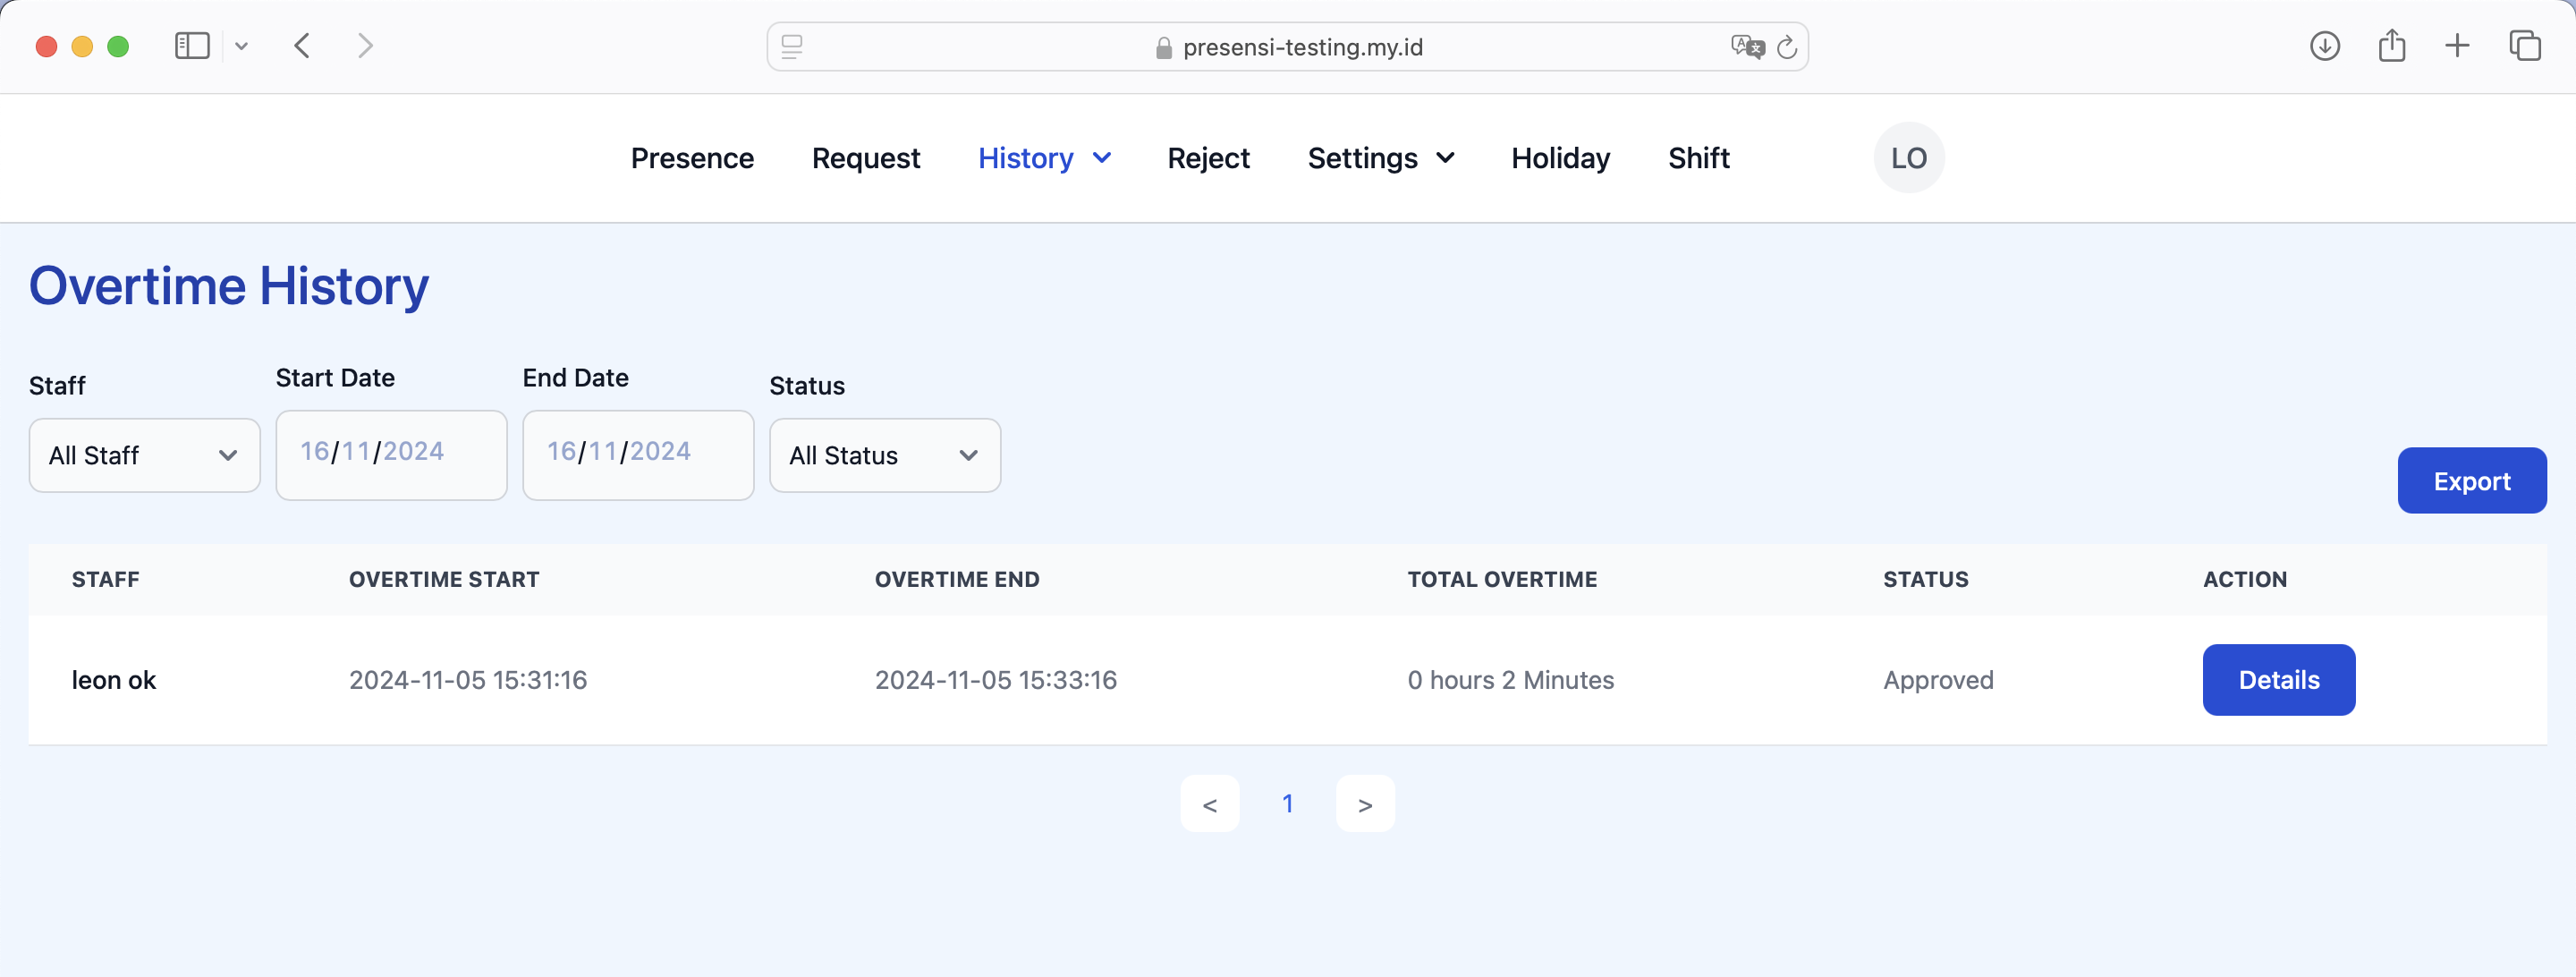
\includegraphics[width=8cm]{Gambar/bab3/user-manual/user-manual-halaman-riwayat-lembur.png}
    	\caption{Halaman \textit{Overtime History}}
    	\label{fig:user-manual-halaman-riwayat-lembur}
        \end{figure}
        \FloatBarrier
    \end{enumerate}

    \item Melihat Detail Riwayat Lembur
    \begin{enumerate}
        \item Membuka halaman riwayat lembur yang terdapat pada \textbf{Manual \ref{item:melihat-riwayat-lembur}}.
        \item Menekan tombol "\textit{Detail}" pada salah satu data lembur. Sistem akan menampilkan modal detail riwayat lembur beserta informasi lengkap riwayat lembur. \textbf{\ref{fig:user-manual-modal-overtime-history-details}} menunjukkan modal \textit{overtime history details}.
        \begin{figure}[!htbp]
    	\centering
    	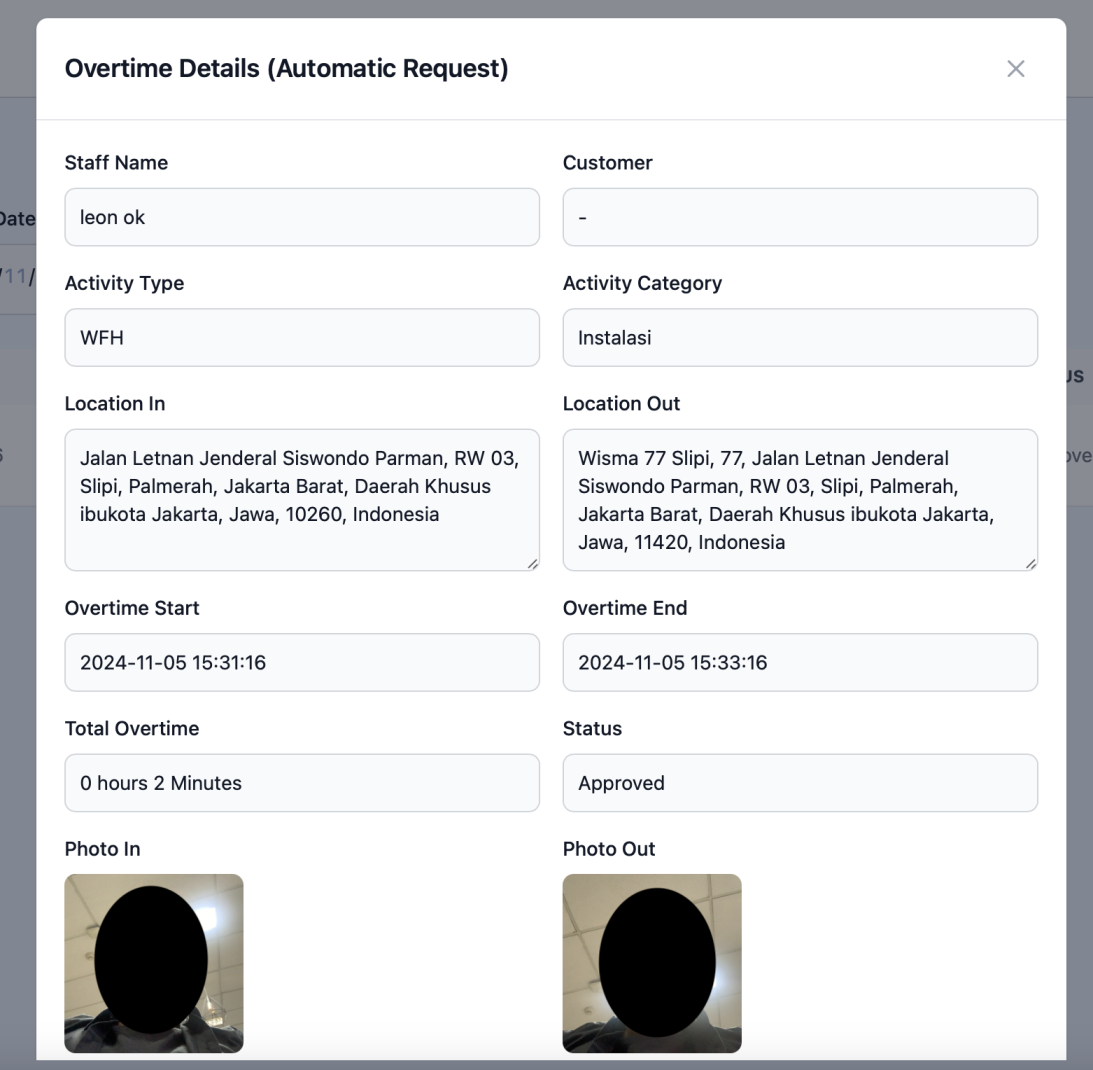
\includegraphics[width=8cm]{Gambar/bab3/user-manual/user-manual-detail-riwayat-lembur.png}
    	\caption{Modal \textit{Overtime History Details}}
    	\label{fig:user-manual-modal-overtime-history-details}
        \end{figure}
        \FloatBarrier
    \end{enumerate}

    \item Melakukan \textit{Export} Data Riwayat Lembur
    \begin{enumerate}
        \item Membuka halaman riwayat lembur yang terdapat pada \textbf{Manual \ref{item:melihat-riwayat-lembur}}.
        \item Menekan tombol \textit{"Export"} yang terdapat pada halaman riwayat lembur. \textbf{\ref{fig:user-manual-tombol-export-riwayat-lembur}} menunjukkan tombol untuk \textit{export} riwayat lembur menjadi format \textit{Excel}.
        \begin{figure}[!htbp]
    	\centering
    	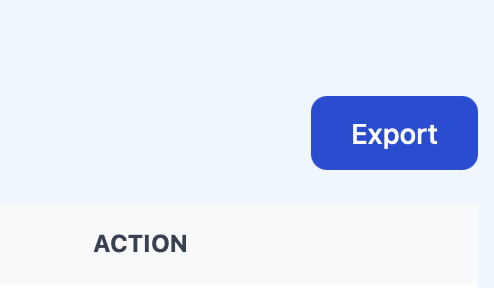
\includegraphics[width=8cm]{Gambar/bab3/user-manual/user-manual-tombol-export-riwayat-lembur.png}
    	\caption{Tombol \textit{Export} Riwayat Lembur}
    	\label{fig:user-manual-tombol-export-riwayat-lembur}
        \end{figure}
        \FloatBarrier
        \item Perangkat akan otomatis men-\textit{download file Excel} yang berisi data lembur. \textbf{\ref{fig:user-manual-file-excel-riwayat-lembur}} menunjukkan \textit{file Excel} riwayat lembur yang telah di-\textit{donwload}.
        \begin{figure}[!htbp]
    	\centering
    	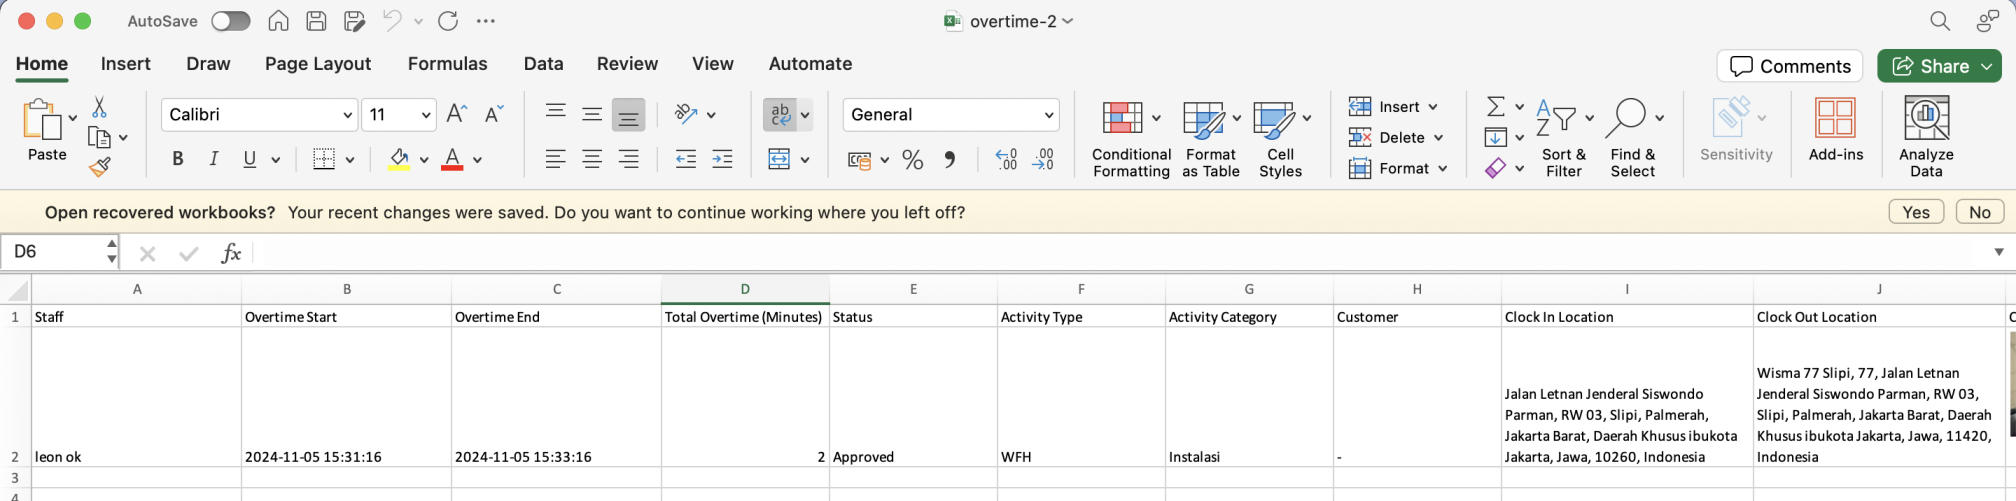
\includegraphics[width=8cm]{Gambar/bab3/user-manual/user-manual-file-excel-riwayat-lembur.png}
    	\caption{\textit{File Excel} Riwayat Lembur}
    	\label{fig:user-manual-file-excel-riwayat-lembur}
        \end{figure}
        \FloatBarrier
    \end{enumerate}
    

    \item Mengakses Halaman \textit{Reject} Lembur\label{item:mengakses-halaman-reject}
    \begin{enumerate}
        \item Melakukan \textit{login} pada aplikasi presensi \textit{online} yang terdapat pada \textbf{Manual \ref{item:melakukan-login}}.
        \item Menekan tombol "\textit{Reject}" pada \textit{navigation bar} yang terletak di paling atas. \textbf{\ref{fig:user-manual-tombol-reject-pada-navigation-bar}} menunjukkan tombol \textit{"Reject"} pada \textit{navigation bar}.
        \begin{figure}[!htbp]
    	\centering
    	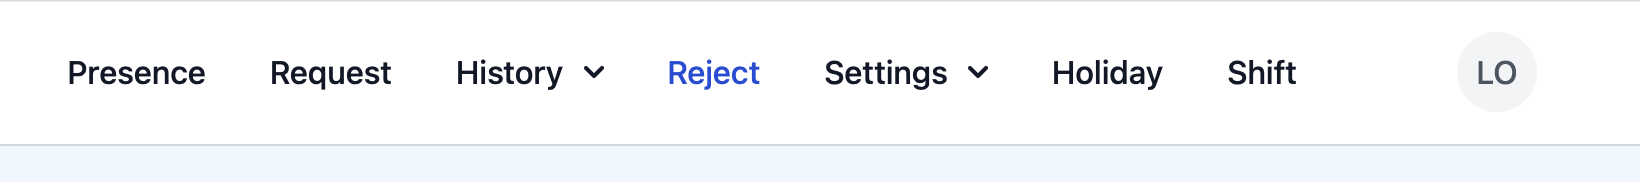
\includegraphics[width=8cm]{Gambar/bab3/user-manual/user-manual-navbar-reject.png}
    	\caption{Tombol \textit{Reject} Pada \textit{Navigation Bar}}
    	\label{fig:user-manual-tombol-reject-pada-navigation-bar}
        \end{figure}
        \FloatBarrier
        \item Sistem akan menampilkan halaman \textit{reject} lembur. \textbf{\ref{fig:user-manual-halaman-reject-lembur}} menunjukkan tampilan halaman \textit{reject lembur}.
        \begin{figure}[!htbp]
    	\centering
    	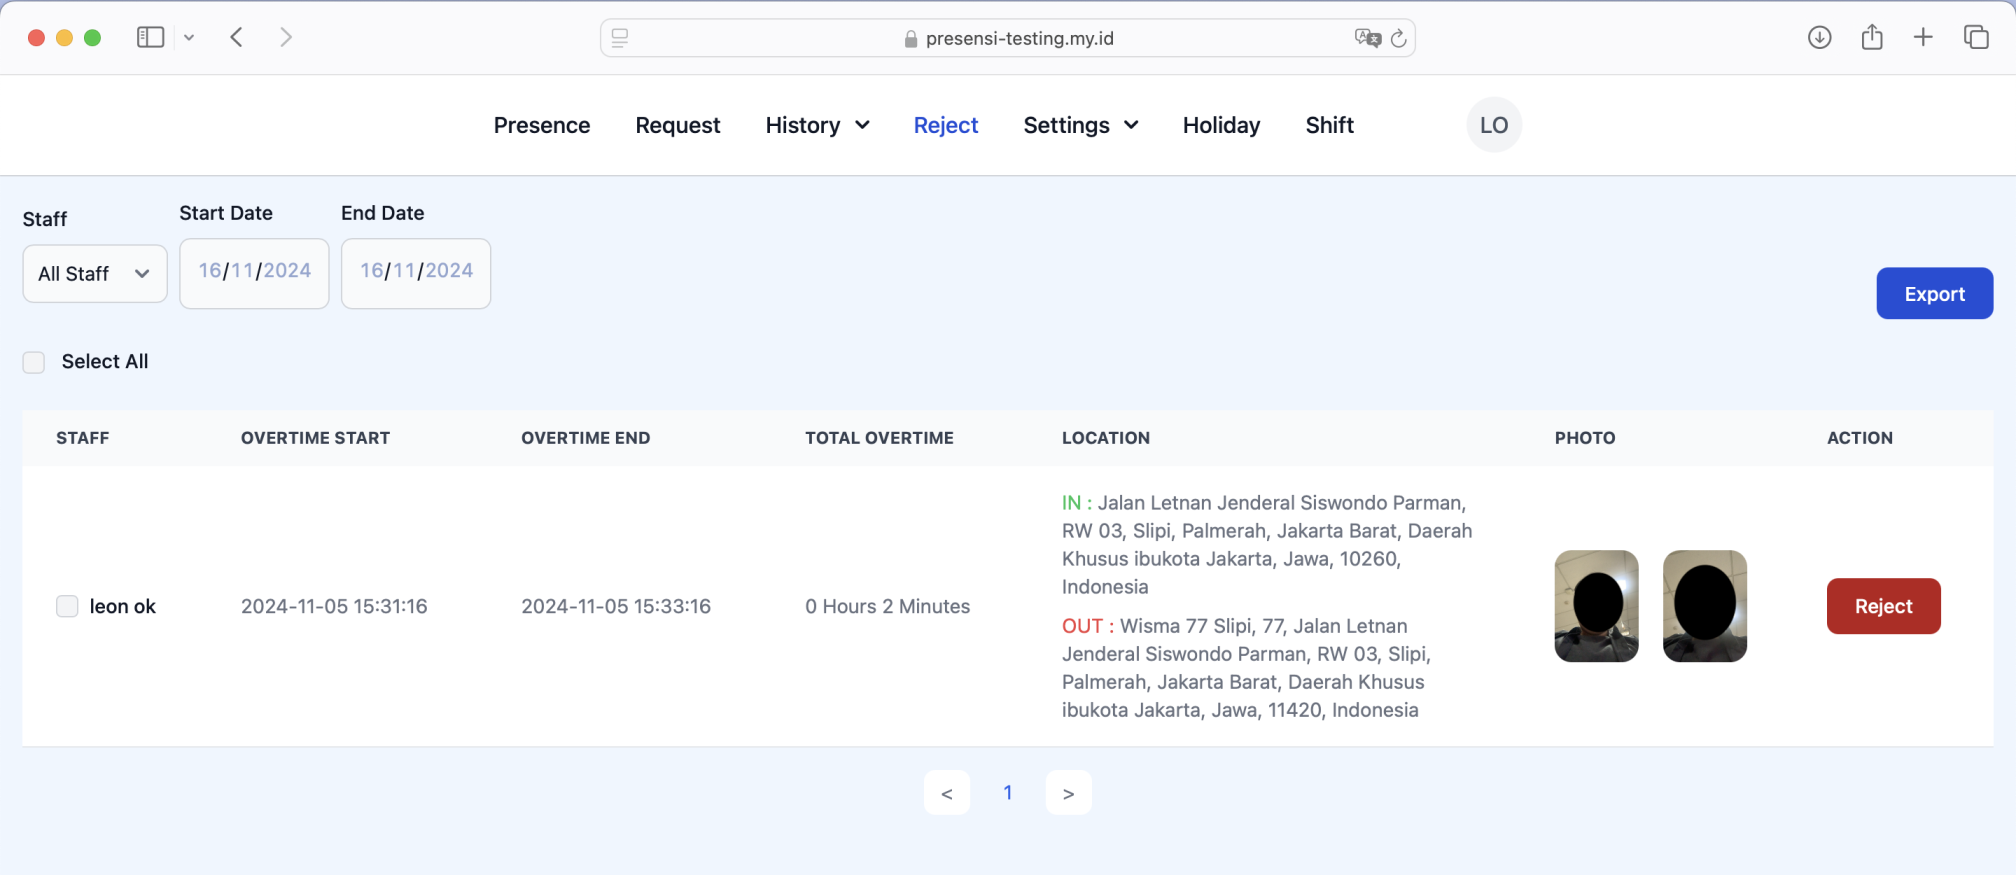
\includegraphics[width=8cm]{Gambar/bab3/user-manual/user-manual-halaman-reject-lembur.png}
    	\caption{Halaman \textit{Reject} Lembur}
    	\label{fig:user-manual-halaman-reject-lembur}
        \end{figure}
        \FloatBarrier
    \end{enumerate}

    \item Melakukan \textit{Reject} Satu Data Lembur
    \begin{enumerate}
        \item Membuka halaman \textit{reject} lembur yang terdapat pada \textbf{Manual \ref{item:mengakses-halaman-reject}}.
        \item Menekan tombol \textit{"Reject"} pada salah satu data lembur dan melakukan konfirmasi. \textbf{\ref{fig:user-manual-tombol-reject-data-lembur}} menunjukkan tombol \textit{"Reject"} pada salah satu data lembur.
        \begin{figure}[!htbp]
    	\centering
    	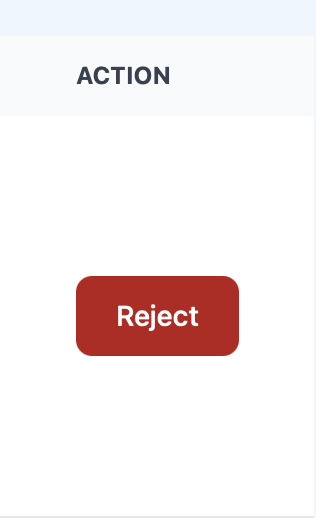
\includegraphics[width=5cm]{Gambar/bab3/user-manual/user-manual-tombol-reject-satu-data-lembur.png}
    	\caption{Tombol \textit{Reject} Pada Data Lembur}
    	\label{fig:user-manual-tombol-reject-data-lembur}
        \end{figure}
        \FloatBarrier
    \end{enumerate}

    \item Melakukan \textit{"Reject"} Lebih Dari Satu Data Lembur
    \begin{enumerate}
        \item Membuka halaman \textit{reject} lembur yang terdapat pada \textbf{Manual \ref{item:mengakses-halaman-reject}}.
        \item Melakukan centang pada \textit{checkbox} data lembur yang akan di-\textit{reject}. \textbf{\ref{fig:user-manual-checkbox-data-lembur}} menunjukkan \textit{checkbox} pada salah satu data lembur.
        \begin{figure}[!htbp]
    	\centering
    	
\includegraphics[width=8cm]{Gambar/bab3/user-manual/user-manual-checkbox-reject-data-lembur.png}
    	\caption{\textit{Checkbox} Data Lembur}
    	\label{fig:user-manual-checkbox-data-lembur}
        \end{figure}
        \FloatBarrier
        \item Setelah memilih \textit{checkbox}, maka akan muncul tombol "\textit{Reject Selected}" untuk me-\textit{reject} seluruh data lembur yang dipilih. \textbf{\ref{fig:user-manual-tombol-reject-selected}} menunjukkan tombol \textit{"Reject Selected"} pada halaman \textit{reject} lembur.
        \begin{figure}[!htbp]
    	\centering
    	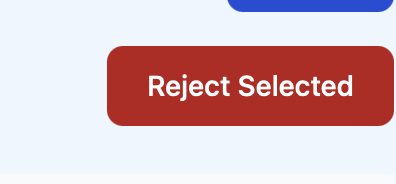
\includegraphics[width=8cm]{Gambar/bab3/user-manual/user-manual-tombol-reject-selected.png}
    	\caption{Tombol \textit{Reject Selected}}
    	\label{fig:user-manual-tombol-reject-selected}
        \end{figure}
        \FloatBarrier
    \end{enumerate}

    \item Melakukan \textit{Export} Data Lembur Pada Halaman \textit{Reject} Lembur
    \begin{enumerate}
        \item Membuka halaman \textit{reject} lembur yang terdapat pada \textbf{Manual \ref{item:mengakses-halaman-reject}}.
        \item Menekan tombol \textit{"Export"} yang terdapat pada halaman \textit{reject} lembur. \textbf{\ref{fig:user-manual-tombol-export-pada-reject-lembur}} menunjukkan tombol "\textit{Export}" pada halaman \textit{reject} lembur.
        \begin{figure}[!htbp]
    	\centering
    	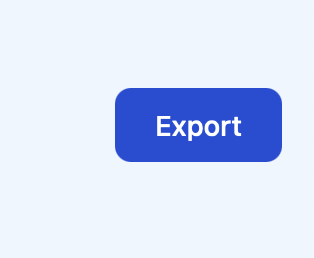
\includegraphics[width=8cm]{Gambar/bab3/user-manual/user-manual-tombol-export-reject-lembur.png}
    	\caption{Tombol \textit{Export} Pada \textit{Reject} Lembur}
    	\label{fig:user-manual-tombol-export-pada-reject-lembur}
        \end{figure}
        \FloatBarrier
        \item Sistem akan otomatis mengunduh \textit{file Excel} yang berisi data lembur dengan status tidak ter-\textit{reject}. \textbf{\ref{fig:user-manual-file-excel-reject-lembur}} menunjukkan \textit{file Excel} yang berisi data lembur yang tidak ter-\textit{reject}.
        \begin{figure}[!htbp]
    	\centering
    	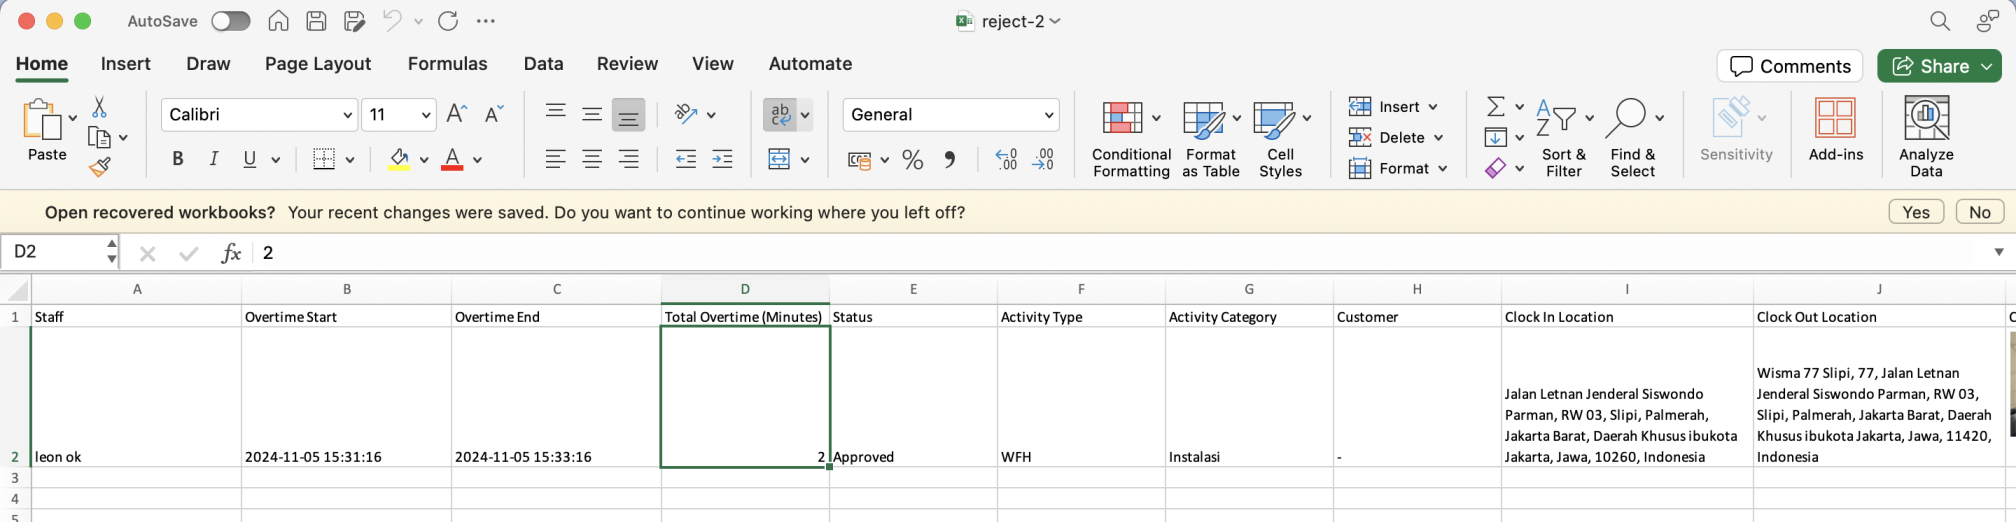
\includegraphics[width=8cm]{Gambar/bab3/user-manual/user-manual-file-excel-reject-lembur.png}
    	\caption{\textit{File Excel Reject} Lembur}
    	\label{fig:user-manual-file-excel-reject-lembur}
        \end{figure}
        \FloatBarrier
    \end{enumerate}

    \item Mengakses Halaman Pengaturan \textit{User}\label{item:mengakses-halaman-pengaturan-user}
    \begin{enumerate}
        \item Melakukan \textit{login} pada aplikasi presensi \textit{online} yang terdapat pada \textbf{Manual \ref{item:melakukan-login}}.
        \item Menekan tombol "\textit{Settings}" pada \textit{navigation bar} yang terletak di paling atas, kemudian tekan tombol "\textit{User}". \textbf{\ref{fig:user-manual-tombol-pengaturan-user-navigation-bar}} menunjukkan tombol \textit{"User"} pada \textit{navigation bar}.
        \begin{figure}[!htbp]
    	\centering
    	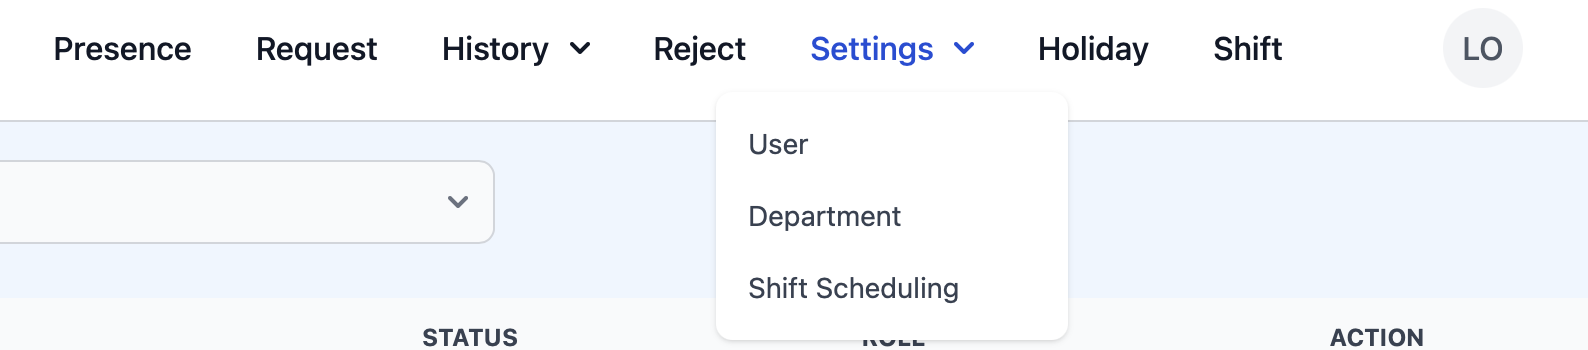
\includegraphics[width=8cm]{Gambar/bab3/user-manual/user-manual-navbar-user.png}
    	\caption{Tombol Pengaturan \textit{User} Pada \textit{Navigation Bar}}
    	\label{fig:user-manual-tombol-pengaturan-user-navigation-bar}
        \end{figure}
        \FloatBarrier
        \item Sistem akan menampilkan data \textit{user} pada halaman pengaturan \textit{user}. \textbf{\ref{fig:user-manual-halaman-pengaturan-user}} menunjukkan halaman pengaturan \textit{user}.
        \begin{figure}[!htbp]
    	\centering
    	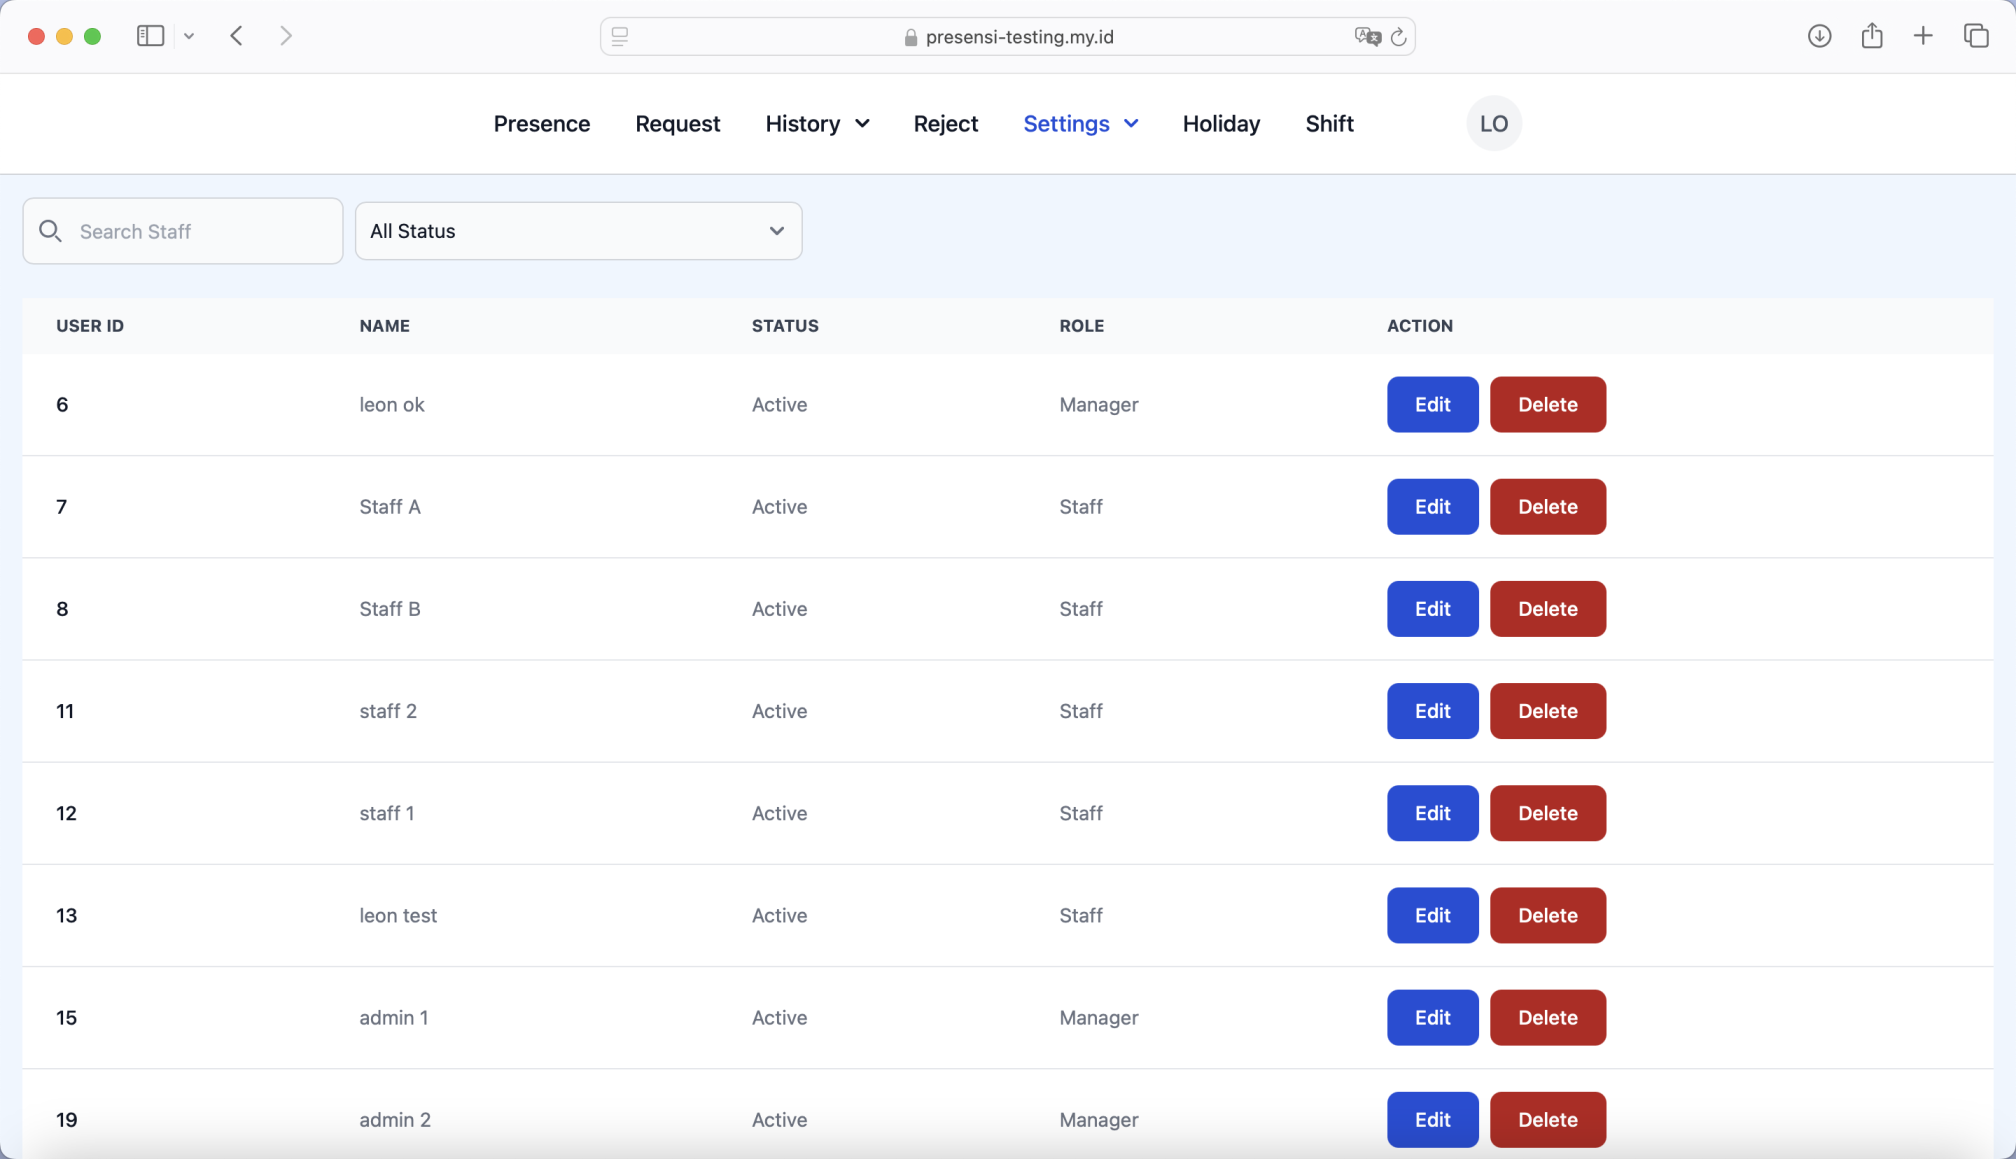
\includegraphics[width=8cm]{Gambar/bab3/user-manual/user-manual-halaman-user.png}
    	\caption{Halaman Pengaturan \textit{User}}
    	\label{fig:user-manual-halaman-pengaturan-user}
        \end{figure}
        \FloatBarrier
    \end{enumerate}

    \item Mengubah Data \textit{User}
    \begin{enumerate}
        \item Membuka halaman pengaturan \textit{user} yang terdapat pada \textbf{Manual \ref{item:mengakses-halaman-pengaturan-user}}. \textbf{\ref{fig:user-manual-tombol-edit-pada-data-user}} menunjukkan tombol "\textit{Edit}" pada data \textit{user}.
        \item Menekan tombol \textit{"Edit"} pada salah satu data \textit{user}.
        \begin{figure}[!htbp]
    	\centering
    	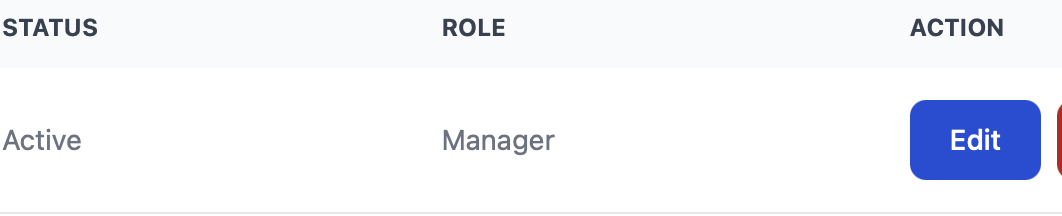
\includegraphics[width=8cm]{Gambar/bab3/user-manual/user-manual-tombol-edit-user.png}
    	\caption{Tombol \textit{Edit} Pada Data \textit{User}}
    	\label{fig:user-manual-tombol-edit-pada-data-user}
        \end{figure}
        \FloatBarrier
        \item Mengubah data \textit{user} melalui \textit{input form} pada modal \textit{edit user}, kemudian tekan tombol "\textit{Save Changes}" untuk menyimpan perubahan data. \textbf{\ref{fig:user-manual-modal-edit-user}} menunjukkan modal \textit{edit user}.
        \begin{figure}[!htbp]
    	\centering
    	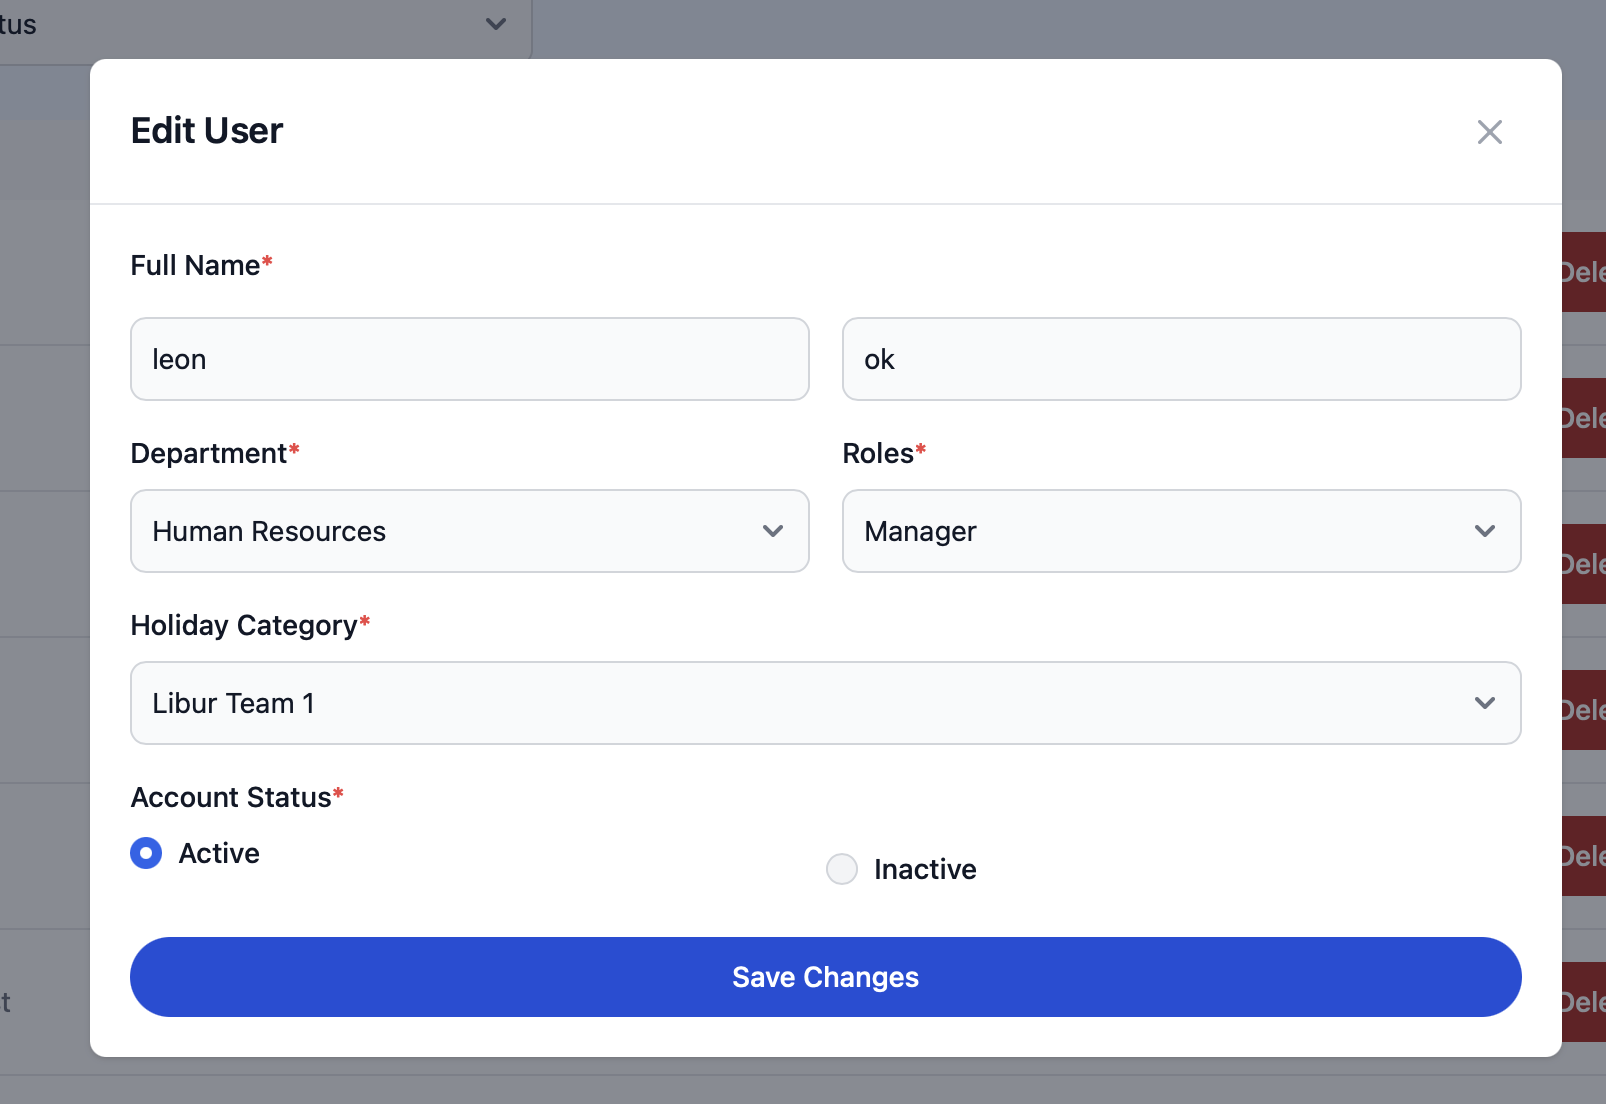
\includegraphics[width=8cm]{Gambar/bab3/user-manual/user-manual-modal-edit-user.png}
    	\caption{Modal \textit{Edit} \textit{User}}
    	\label{fig:user-manual-modal-edit-user}
        \end{figure}
        \FloatBarrier
    \end{enumerate}

    \item Menghapus Data \textit{User}
    \begin{enumerate}
        \item Membuka halaman pengaturan \textit{user} yang terdapat pada \textbf{Manual \ref{item:mengakses-halaman-pengaturan-user}}.
        \item Menekan tombol "\textit{Delete}" pada salah satu data \textit{user} dan lakukan konfirmasi penghapusan. \textbf{\ref{fig:user-manual-tombol-delete-user}} menunjukkan tombol "\textit{Delete}" untuk menghapus data \textit{user}.
        \begin{figure}[!htbp]
    	\centering
    	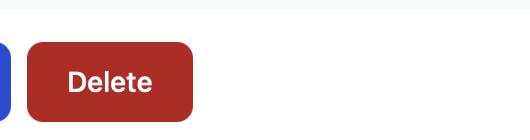
\includegraphics[width=8cm]{Gambar/bab3/user-manual/user-manual-tombol-delete-user.png}
    	\caption{Tombol \textit{Delete User}}
    	\label{fig:user-manual-tombol-delete-user}
        \end{figure}
        \FloatBarrier
    \end{enumerate}

    \item Mengakses Halaman \textit{Department}\label{item:mengakses-department}
    \begin{enumerate}
        \item Melakukan \textit{login} pada aplikasi presensi \textit{online} yang terdapat pada \textbf{Manual \ref{item:melakukan-login}}.
        \item Menekan tombol "\textit{Settings}" pada \textit{navigation bar} yang terletak di paling atas, kemudian tekan tombol "\textit{Department}". \textbf{\ref{fig:user-manual-tombol-pengaturan-department-navigation-bar}} menunjukkan tombol \textit{"Department"} pada \textit{navigation bar}.
        \begin{figure}[!htbp]
    	\centering
    	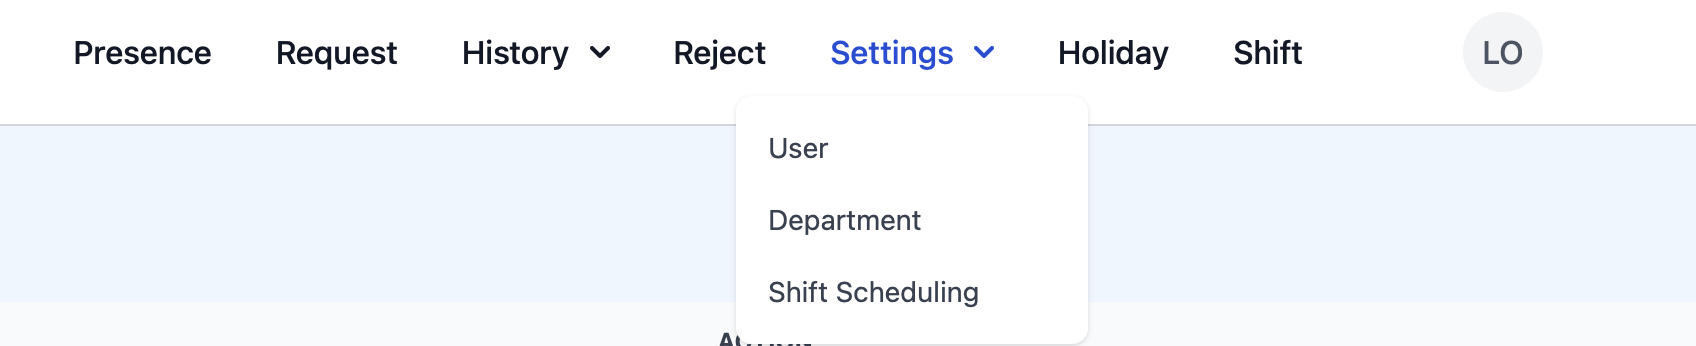
\includegraphics[width=8cm]{Gambar/bab3/user-manual/user-manual-navbar-department.png}
    	\caption{Tombol Pengaturan \textit{Department} Pada \textit{Navigation Bar}}
    	\label{fig:user-manual-tombol-pengaturan-department-navigation-bar}
        \end{figure}
        \FloatBarrier
        \item Sistem akan menampilkan data \textit{department} pada halaman pengaturan \textit{department}. \textbf{\ref{fig:user-manual-halaman-pengaturan-department}} menunjukkan halaman pengaturan \textit{department}.
        \begin{figure}[!htbp]
    	\centering
    	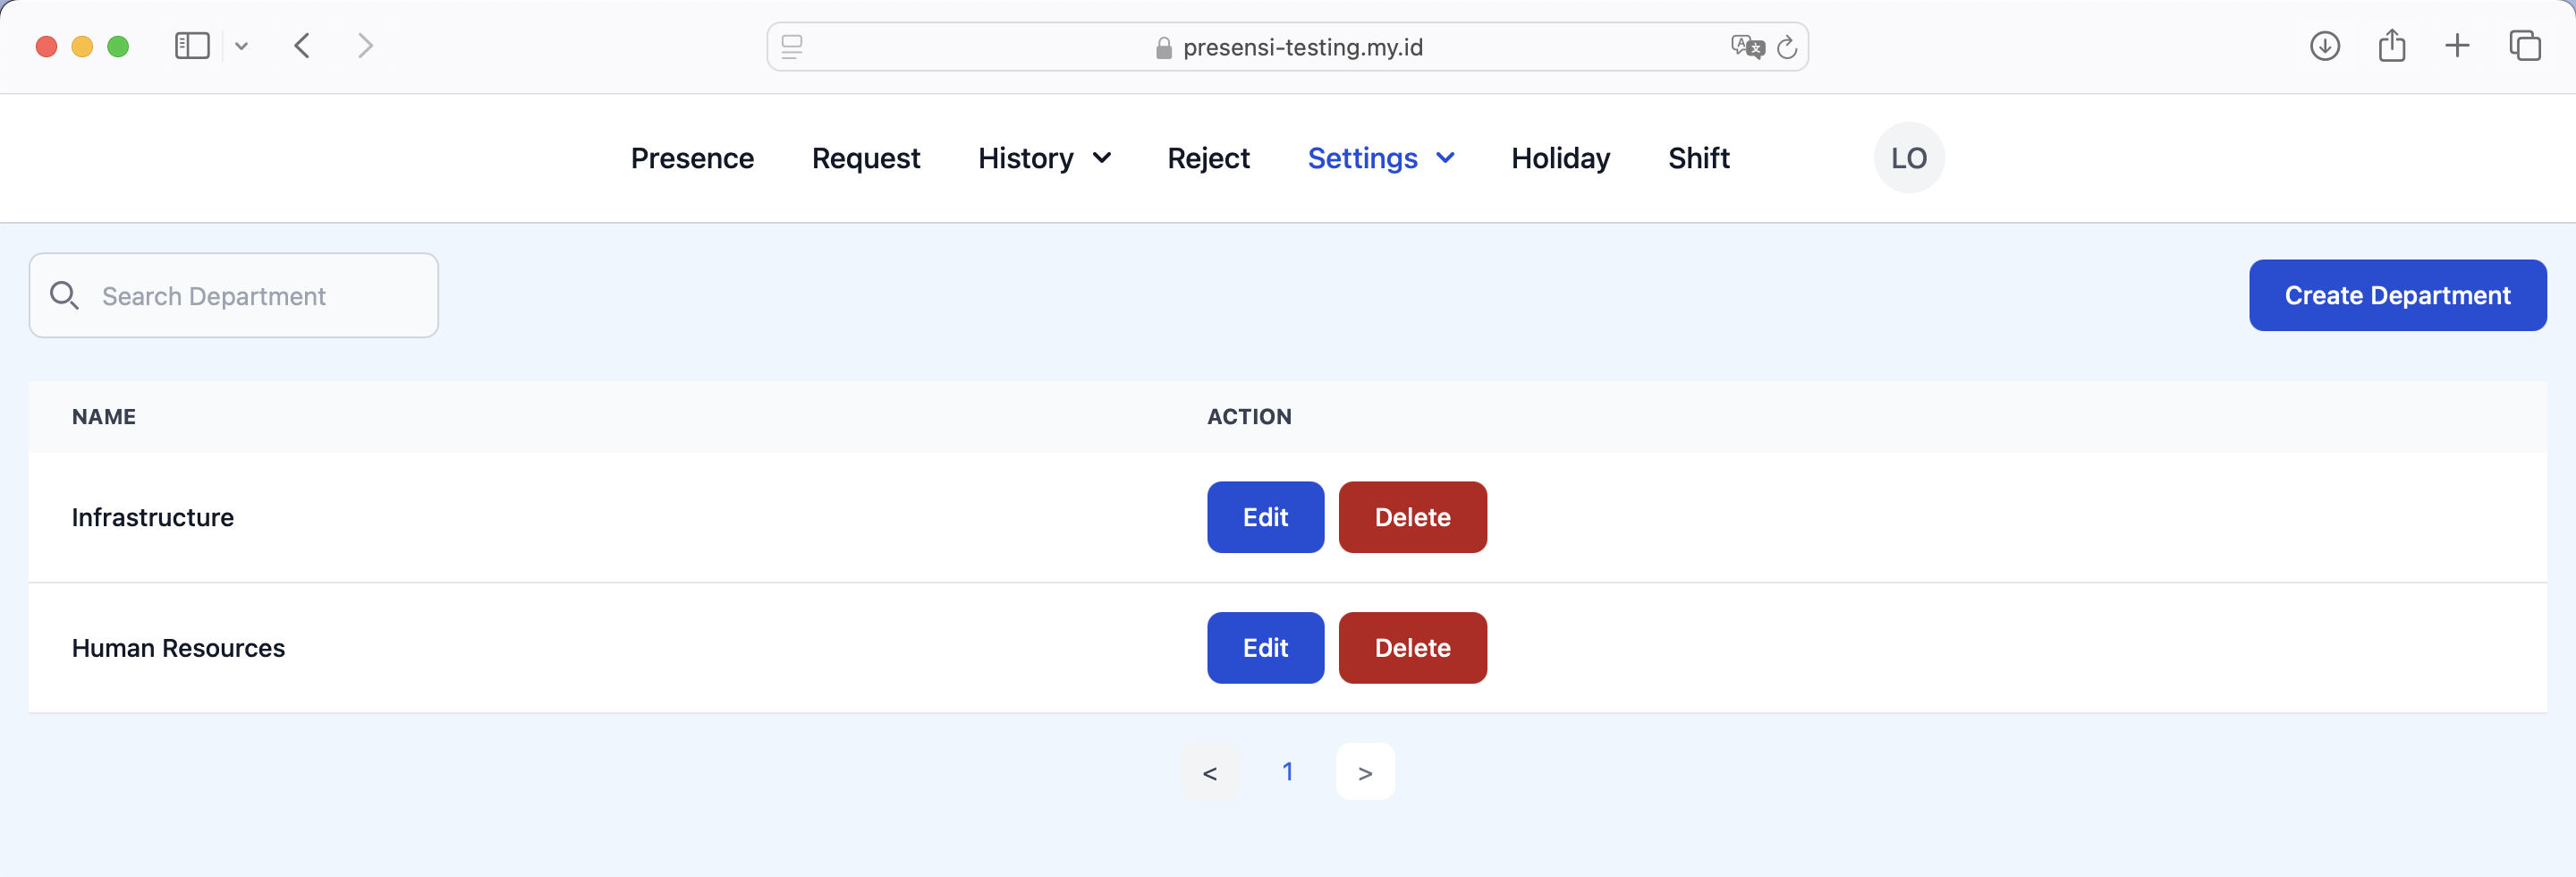
\includegraphics[width=8cm]{Gambar/bab3/user-manual/user-manual-halaman-department.png}
    	\caption{Halaman Pengaturan \textit{Department}}
    	\label{fig:user-manual-halaman-pengaturan-department}
        \end{figure}
        \FloatBarrier
    \end{enumerate}

    \item Menambah \textit{Department}
    \begin{enumerate}
        \item Membuka halaman pengaturan \textit{department} yang terdapat pada \textbf{Manual \ref{item:mengakses-department}}.
        \item Menekan tombol "\textit{Create Department}" pada halaman pengaturan \textit{department}. \textbf{\ref{fig:user-manual-tombol-create-new-department}} menunjukkan tombol "\textit{Create Department}" pada halaman pengaturan \textit{department}.
        \begin{figure}[!htbp]
    	\centering
    	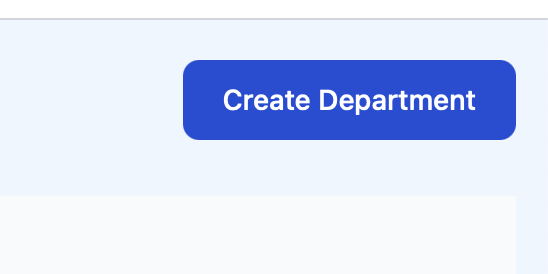
\includegraphics[width=8cm]{Gambar/bab3/user-manual/user-manual-tombol-create-new-department.png}
    	\caption{Tombol \textit{Create Department}}
    	\label{fig:user-manual-tombol-create-new-department}
        \end{figure}
        \FloatBarrier

        \item Mengisi seluruh \textit{input form} pada modal \textit{create new department}, kemudian tekan tombol "\textit{Create New Department}" untuk menyimpan data \textit{department} baru. \textbf{\ref{fig:user-manual-modal-create-new-department}} menunjukkan modal \textit{create new department}.
        \begin{figure}[!htbp]
    	\centering
    	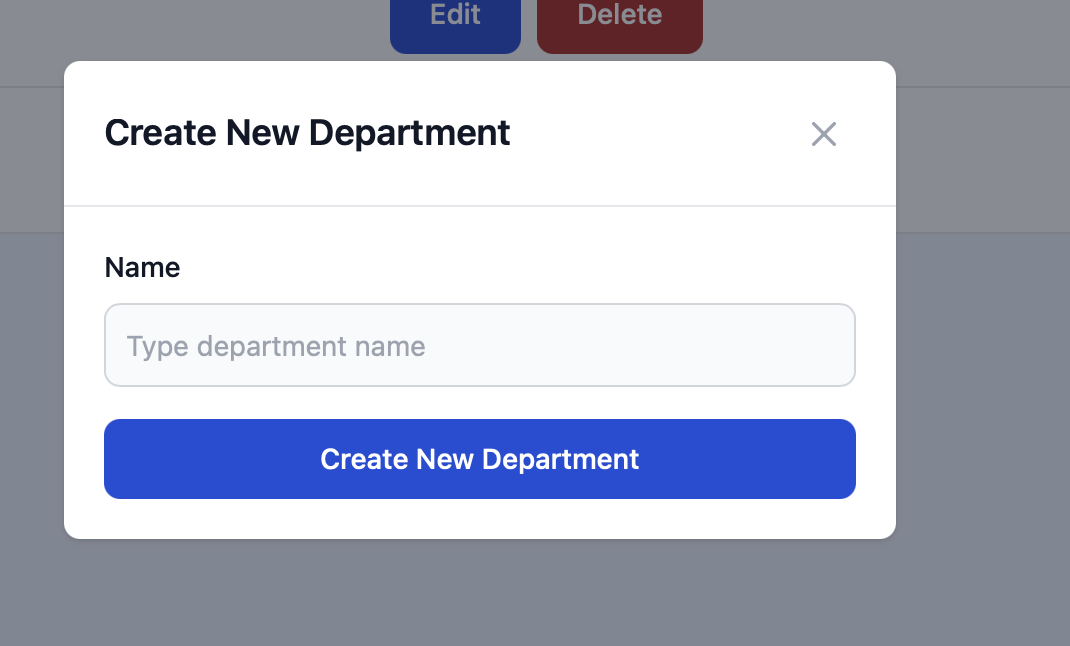
\includegraphics[width=8cm]{Gambar/bab3/user-manual/user-manual-modal-create-new-department.png}
    	\caption{Modal \textit{Create New Department}}
    	\label{fig:user-manual-modal-create-new-department}
        \end{figure}
        \FloatBarrier
    \end{enumerate}

    \item Mengubah \textit{Department}
    \begin{enumerate}
        \item Membuka halaman pengaturan \textit{department} yang terdapat pada \textbf{Manual \ref{item:mengakses-department}}.
        \item Menekan tombol "\textit{Edit}" salah satu data \textit{department} pada halaman pengaturan \textit{department}. \textbf{\ref{fig:user-manual-tombol-edit-department}} menunjukkan tombol "\textit{Edit}" pada halaman pengaturan \textit{department}.
        \begin{figure}[!htbp]
    	\centering
    	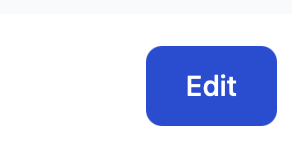
\includegraphics[width=8cm]{Gambar/bab3/user-manual/user-manual-tombol-edit-department.png}
    	\caption{Tombol \textit{Edit} Department}
    	\label{fig:user-manual-tombol-edit-department}
        \end{figure}
        \FloatBarrier

        \item Mengubah seluruh \textit{input form} pada modal \textit{edit department}, kemudian tekan tombol "\textit{Save Changes}" untuk menyimpan data \textit{department}. \textbf{\ref{fig:user-manual-modal-edit-department}} menunjukkan modal \textit{edit department}.
        \begin{figure}[!htbp]
    	\centering
    	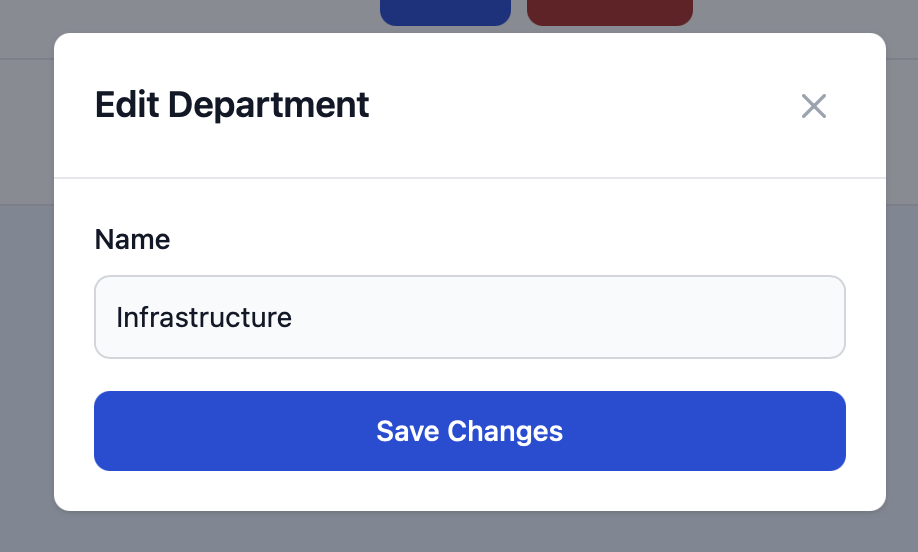
\includegraphics[width=8cm]{Gambar/bab3/user-manual/user-manual-modal-edit-department.png}
    	\caption{Modal \textit{Edit Department}}
    	\label{fig:user-manual-modal-edit-department}
        \end{figure}
        \FloatBarrier
    \end{enumerate}

    \item Menghapus Data \textit{Department}
    \begin{enumerate}
        \item Membuka halaman pengaturan \textit{department} yang terdapat pada \textbf{Manual \ref{item:mengakses-department}}.
        \item Menekan tombol "\textit{Delete}" pada salah satu data \textit{department} dan lakukan konfirmasi penghapusan. \textbf{\ref{fig:user-manual-tombol-delete-department}} menunjukkan tombol "\textit{Delete}" untuk menghapus data \textit{department}.
        \begin{figure}[!htbp]
    	\centering
    	
\includegraphics[width=8cm]{Gambar/bab3/user-manual/user-manual-tombol-delete-department.png}
    	\caption{Tombol \textit{Delete Department}}
    	\label{fig:user-manual-tombol-delete-department}
        \end{figure}
        \FloatBarrier
    \end{enumerate}

    \item Mengakses Halaman Penjadwalan \textit{Shift}\label{item:mengakses-shift-scheduling}
    \begin{enumerate}
        \item Melakukan \textit{login} pada aplikasi presensi \textit{online} yang terdapat pada \textbf{Manual \ref{item:melakukan-login}}.
        \item Menekan tombol "\textit{Settings}" pada \textit{navigation bar} yang terletak di paling atas, kemudian tekan tombol "\textit{Shift Scheduling}". \textbf{\ref{fig:user-manual-tombol-pengaturan-shift-scheduling-navigation-bar}} menunjukkan tombol \textit{"Shift Scheduling"} pada \textit{navigation bar}.
        \begin{figure}[!htbp]
    	\centering
    	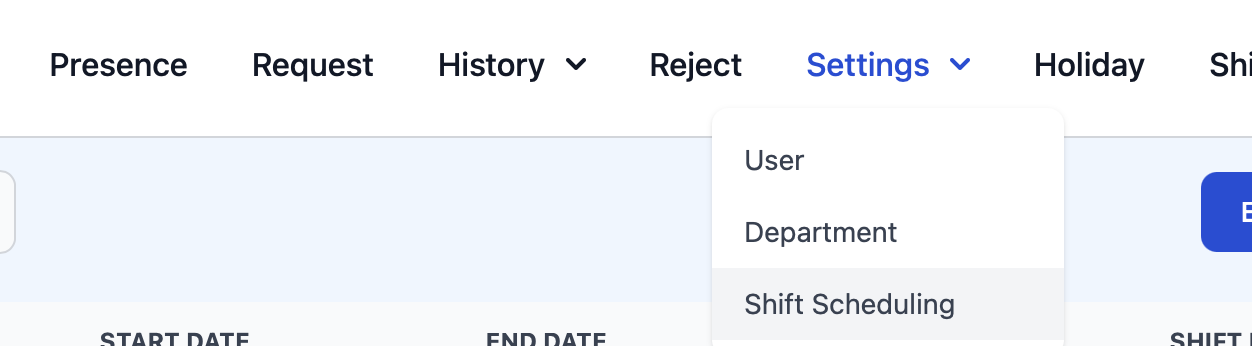
\includegraphics[width=8cm]{Gambar/bab3/user-manual/user-manual-navbar-shift-scheduling.png}
    	\caption{Tombol Pengaturan \textit{Shift Scheduling} Pada \textit{Navigation Bar}}
    	\label{fig:user-manual-tombol-pengaturan-shift-scheduling-navigation-bar}
        \end{figure}
        \FloatBarrier
        \item Sistem akan menampilkan data penjadwalan \textit{shift} pada halaman pengaturan \textit{shift scheduling}. \textbf{\ref{fig:user-manual-halaman-pengaturan-shift-scheduling}} menunjukkan halaman pengaturan \textit{shift scheduling}.
        \begin{figure}[!htbp]
    	\centering
    	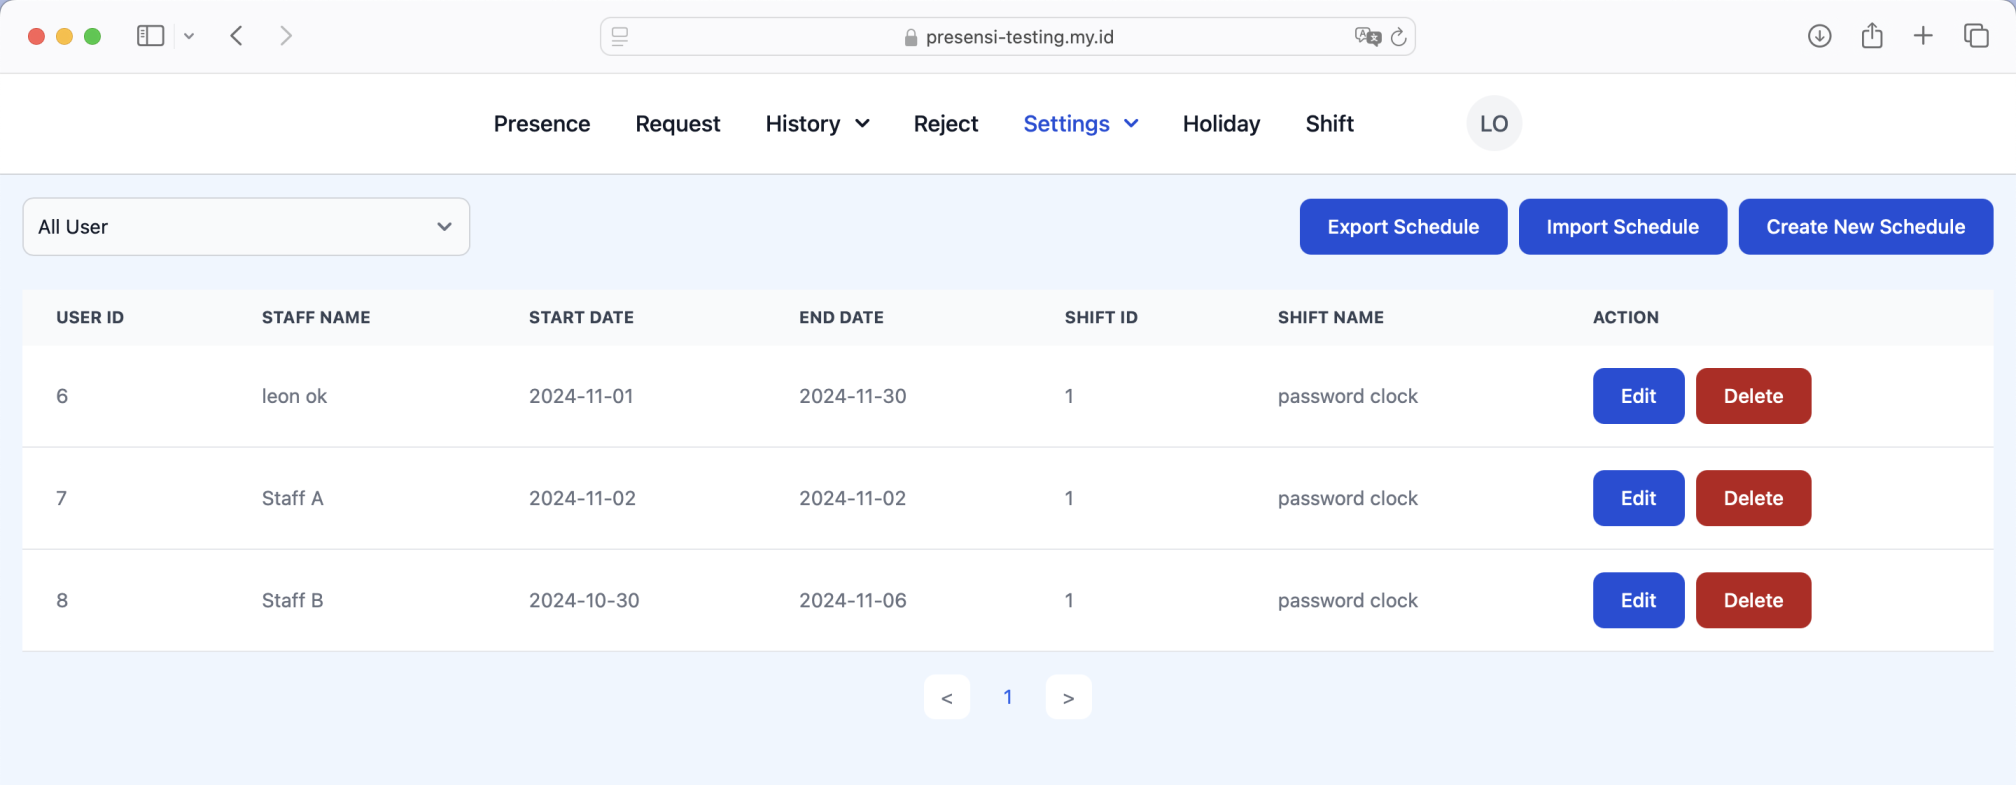
\includegraphics[width=8cm]{Gambar/bab3/user-manual/user-manual-halaman-shift-scheduling.png}
    	\caption{Halaman Pengaturan \textit{Shift Scheduling}}
    	\label{fig:user-manual-halaman-pengaturan-shift-scheduling}
        \end{figure}
        \FloatBarrier
    \end{enumerate}

    \item Menambah Data Penjadwalan \textit{Shift}
    \begin{enumerate}
        \item Membuka halaman \textit{shift scheduling} yang terdapat pada \textbf{Manual \ref{item:mengakses-shift-scheduling}}.
        \item Menekan tombol "\textit{Create New Schedule}" pada halaman pengaturan \textit{shift scheduling}. \textbf{\ref{fig:user-manual-tombol-create-new-schedule}} menunjukkan tombol "\textit{Create New Schedule}" pada halaman pengaturan \textit{shift scheduling}.
        \begin{figure}[!htbp]
    	\centering
    	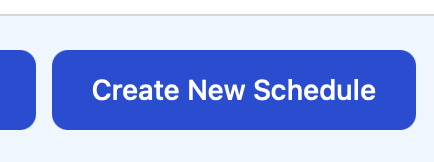
\includegraphics[width=8cm]{Gambar/bab3/user-manual/user-manual-tombol-create-new-schedule.png}
    	\caption{Tombol \textit{Create New Schedule}}
    	\label{fig:user-manual-tombol-create-new-schedule}
        \end{figure}
        \FloatBarrier

        \item Mengisi seluruh \textit{input form} pada modal \textit{create new schedule}, kemudian tekan tombol "\textit{Create New Schedule}" untuk menyimpan data penjadwalan \textit{shift} baru. \textbf{\ref{fig:user-manual-modal-create-new-schedule}} menunjukkan modal \textit{create new schedule}.
        \begin{figure}[!htbp]
    	\centering
    	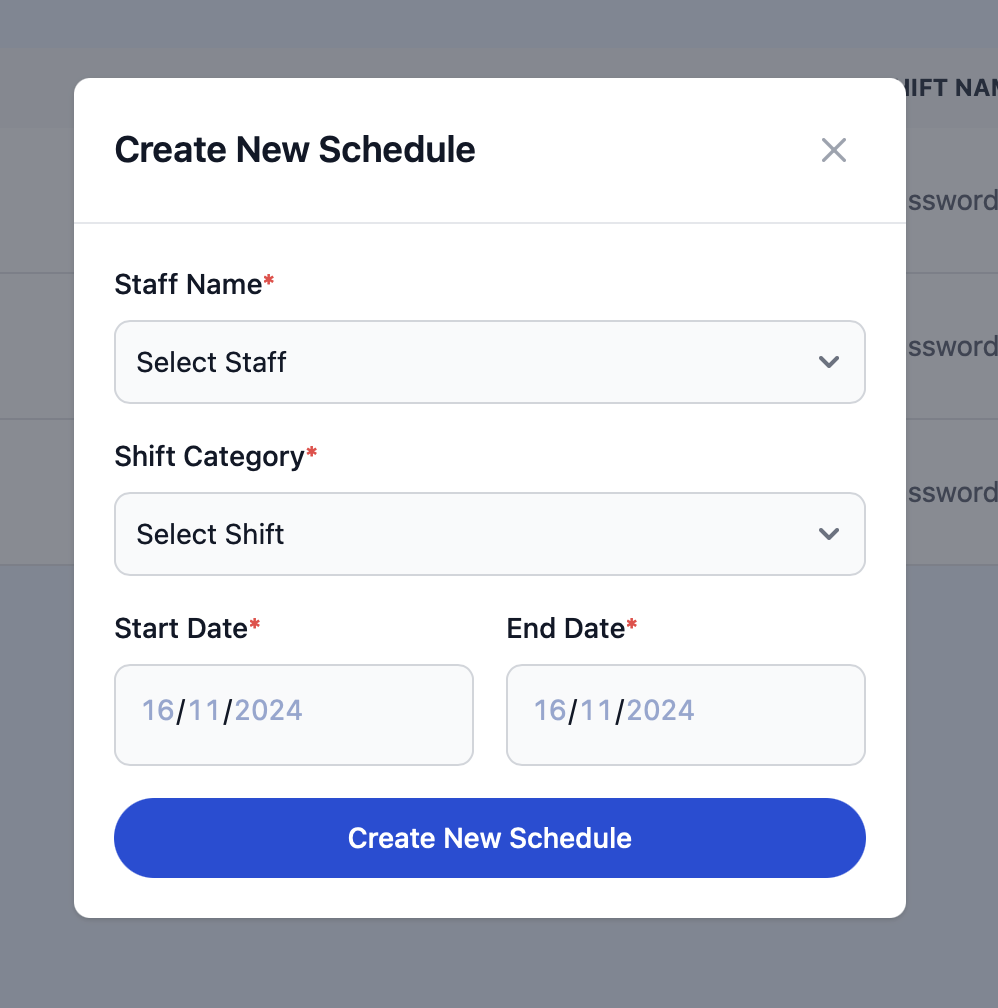
\includegraphics[width=8cm]{Gambar/bab3/user-manual/user-manual-modal-create-new-schedule.png}
    	\caption{Modal \textit{Create New Schedule}}
    	\label{fig:user-manual-modal-create-new-schedule}
        \end{figure}
        \FloatBarrier
    \end{enumerate}

    \item Mengubah Data Penjadwalan \textit{Shift}
    \begin{enumerate}
        \item Membuka halaman \textit{shift scheduling} yang terdapat pada \textbf{Manual \ref{item:mengakses-shift-scheduling}}.
        \item Menekan tombol "\textit{Edit}" salah satu data \textit{shift scheduling} pada halaman pengaturan \textit{shift scheduling}. \textbf{\ref{fig:user-manual-tombol-edit-schedule}} menunjukkan tombol "\textit{Edit}" pada halaman pengaturan \textit{shift scheduling}.
        \begin{figure}[!htbp]
    	\centering
    	
\includegraphics[width=8cm]{Gambar/bab3/user-manual/user-manual-tombol-edit-schedule.png}
    	\caption{Tombol \textit{Edit Schedule}}
    	\label{fig:user-manual-tombol-edit-schedule}
        \end{figure}
        \FloatBarrier

        \item Mengubah seluruh \textit{input form} pada modal \textit{edit schedule}, kemudian tekan tombol "\textit{Edit Schedule}" untuk menyimpan data \textit{shift scheduling}. \textbf{\ref{fig:user-manual-modal-edit-schedule}} menunjukkan modal \textit{edit schedule}.
        \begin{figure}[!htbp]
    	\centering
    	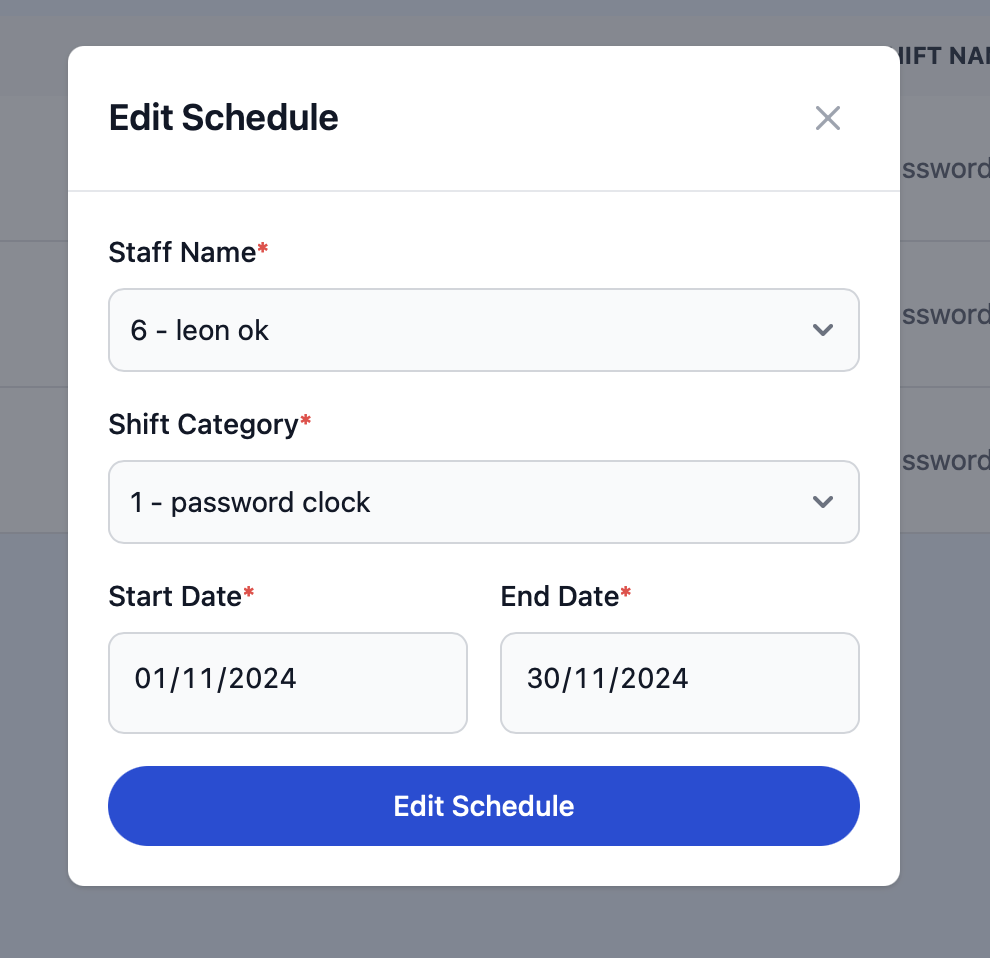
\includegraphics[width=8cm]{Gambar/bab3/user-manual/user-manual-modal-edit-schedule.png}
    	\caption{Modal \textit{Edit Schedule}}
    	\label{fig:user-manual-modal-edit-schedule}
        \end{figure}
        \FloatBarrier
    \end{enumerate}

    \item Menghapus Data Penjadwalan \textit{Shift}
    \begin{enumerate}
        \item Membuka halaman \textit{shift scheduling} yang terdapat pada \textbf{Manual \ref{item:mengakses-shift-scheduling}}.
        \item Menekan tombol "\textit{Delete}" pada salah satu data \textit{shift scheduling} dan lakukan konfirmasi penghapusan. \textbf{\ref{fig:user-manual-tombol-delete-shift-scheduling}} menunjukkan tombol "\textit{Delete}" untuk menghapus data \textit{shift scheduling}.
        \begin{figure}[!htbp]
    	\centering
    	
\includegraphics[width=8cm]{Gambar/bab3/user-manual/user-manual-tombol-delete-schedule.png}
    	\caption{Tombol \textit{Delete Shift Scheduling}}
    	\label{fig:user-manual-tombol-delete-shift-scheduling}
        \end{figure}
        \FloatBarrier
    \end{enumerate}

    \item Melakukan \textit{Export} Data Penjadwalan \textit{Shift}\label{item:export-shift-scheduling}
    \begin{enumerate}
        \item Membuka halaman \textit{shift scheduling} yang terdapat pada \textbf{Manual \ref{item:mengakses-shift-scheduling}}.
        \item Menekan tombol "\textit{Export Schedule}" pada halaman \textit{shift scheduling}. \textbf{\ref{fig:user-manual-tombol-export-shift-scheduling}} menunjukkan tombol \textit{"Export Schedule"} untuk men-\textit{download} data \textit{shift scheduling}.
        \begin{figure}[!htbp]
    	\centering
    	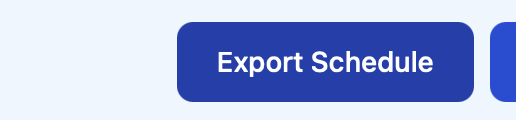
\includegraphics[width=8cm]{Gambar/bab3/user-manual/user-manual-tombol-export-shift-scheduling.png}
    	\caption{Tombol \textit{Export Shift Scheduling}}
    	\label{fig:user-manual-tombol-export-shift-scheduling}
        \end{figure}
        \FloatBarrier
        \item Sistem akan otomatis mengunduh \textit{file Excel} yang berisi seluruh data \textit{shift scheduling}. \textbf{\ref{fig:user-manual-file-excel-shift-scheduling}} menunjukkan \textit{file Excel} yang berisi seluruh data \textit{shift scheduling}.
        \begin{figure}[!htbp]
    	\centering
    	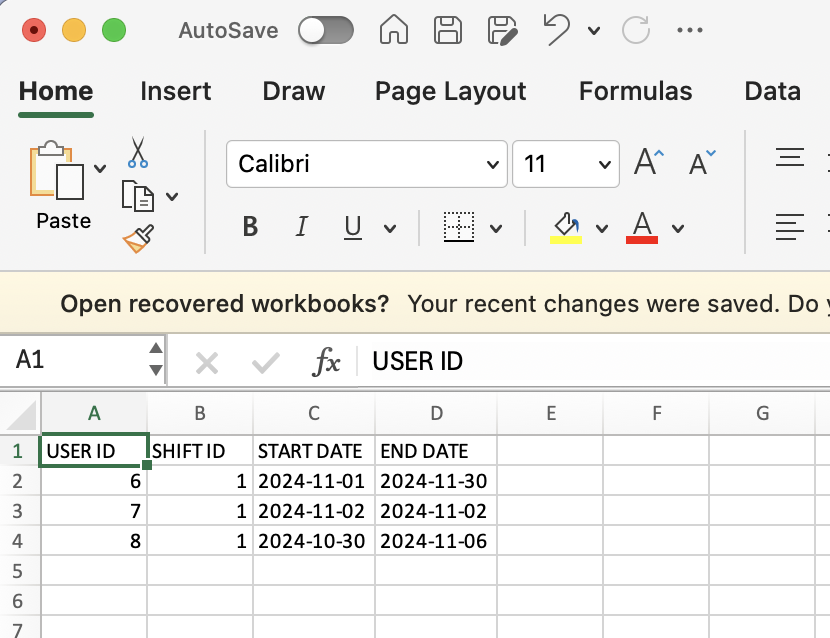
\includegraphics[width=8cm]{Gambar/bab3/user-manual/user-manual-file-excel-shift-scheduling.png}
    	\caption{\textit{File Excel} \textit{Shift Scheduling}}
    	\label{fig:user-manual-file-excel-shift-scheduling}
        \end{figure}
        \FloatBarrier
    \end{enumerate}

    \item Melakukan \textit{Import} Penjadwalan \textit{Shift}
    \begin{enumerate}
        \item Membuka halaman \textit{shift scheduling} yang terdapat pada \textbf{Manual \ref{item:mengakses-shift-scheduling}}.
        \item Menekan tombol "\textit{Import Schedule}" pada halaman \textit{shift scheduling}. \textbf{\ref{fig:user-manual-tombol-import-shift-scheduling}} menunjukkan tombol \textit{"Import Schedule"}.
        \begin{figure}[!htbp]
    	\centering
    	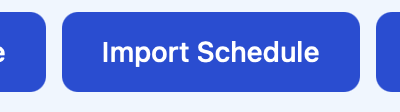
\includegraphics[width=8cm]{Gambar/bab3/user-manual/user-manual-tombol-import-shift-scheduling.png}
    	\caption{Tombol \textit{Import Shift Scheduling}}
    	\label{fig:user-manual-tombol-import-shift-scheduling}
        \end{figure}
        \FloatBarrier
        \item Meng-\textit{upload} dan mengubah isi \textit{file Excel} yang telah diunduh dari \textbf{Manual \ref{item:export-shift-scheduling}}, kemudian tekan tombol "\textit{Import Now}" untuk me-\textit{replace} seluruh \textit{shift scheduling}. \textbf{\ref{fig:user-manual-modal-import-shift-scheduling}} menunjukkan modal \textit{import shift scheduling}.
        \begin{figure}[!htbp]
    	\centering
    	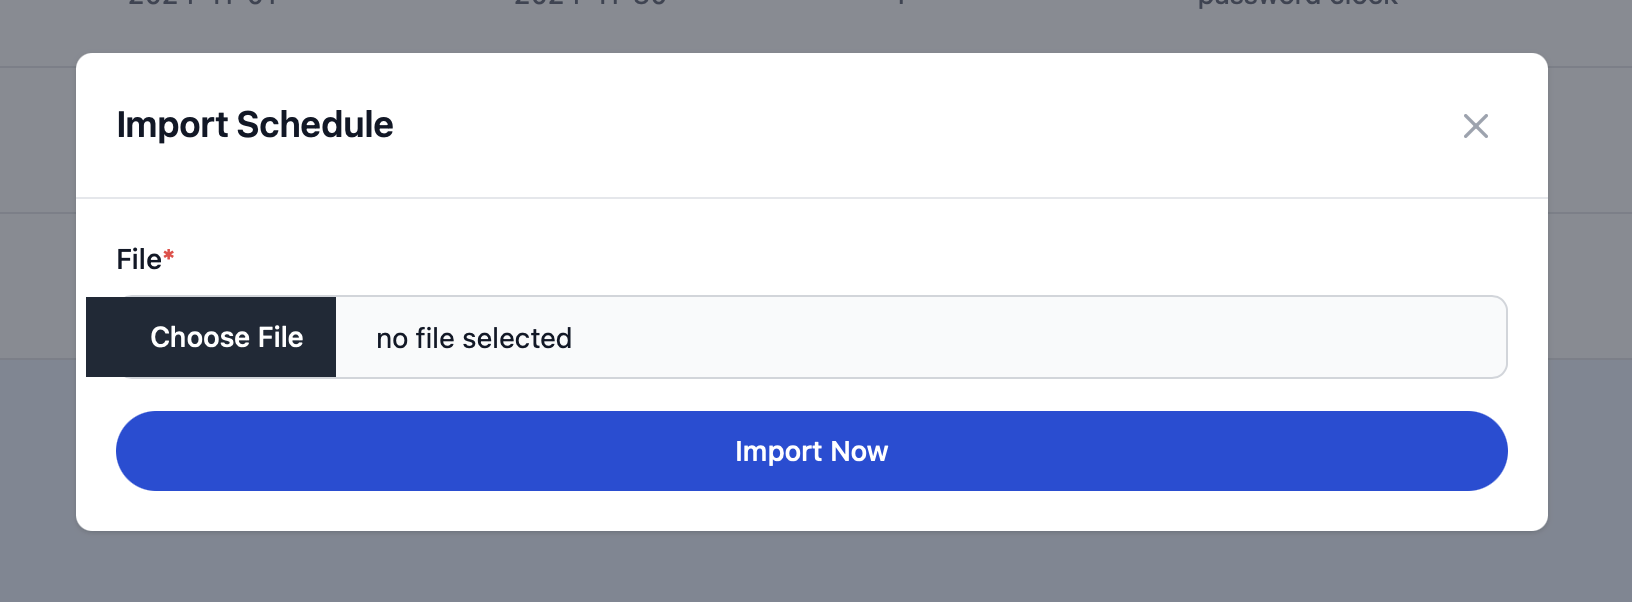
\includegraphics[width=8cm]{Gambar/bab3/user-manual/user-manual-modal-import-shift-scheduling.png}
    	\caption{Modal \textit{Import Shift Scheduling}}
    	\label{fig:user-manual-modal-import-shift-scheduling}
        \end{figure}
        \FloatBarrier
    \end{enumerate}


    \item Mengakses Halaman Jenis Libur Perusahaan\label{item:mengakses-jenis-libur-perusahaan}
    \begin{enumerate}
        \item Melakukan \textit{login} pada aplikasi presensi \textit{online} yang terdapat pada \textbf{Manual \ref{item:melakukan-login}}.
        \item Menekan tombol "\textit{Holiday}" pada \textit{navigation bar} yang terletak di paling atas. \textbf{\ref{fig:user-manual-tombol-holiday-navigation-bar}} menunjukkan tombol \textit{"Holiday"} pada \textit{navigation bar}.
        \begin{figure}[!htbp]
    	\centering
    	
\includegraphics[width=8cm]{Gambar/bab3/user-manual/user-manual-navbar-holiday.png}
    	\caption{Tombol \textit{Holiday} Pada \textit{Navigation Bar}}
    	\label{fig:user-manual-tombol-holiday-navigation-bar}
        \end{figure}
        \FloatBarrier
        \item Sistem akan menampilkan data jenis libur perusahaan pada halaman \textit{holiday}. \textbf{\ref{fig:user-manual-halaman-holiday}} menunjukkan halaman \textit{holiday}.
        \begin{figure}[!htbp]
    	\centering
    	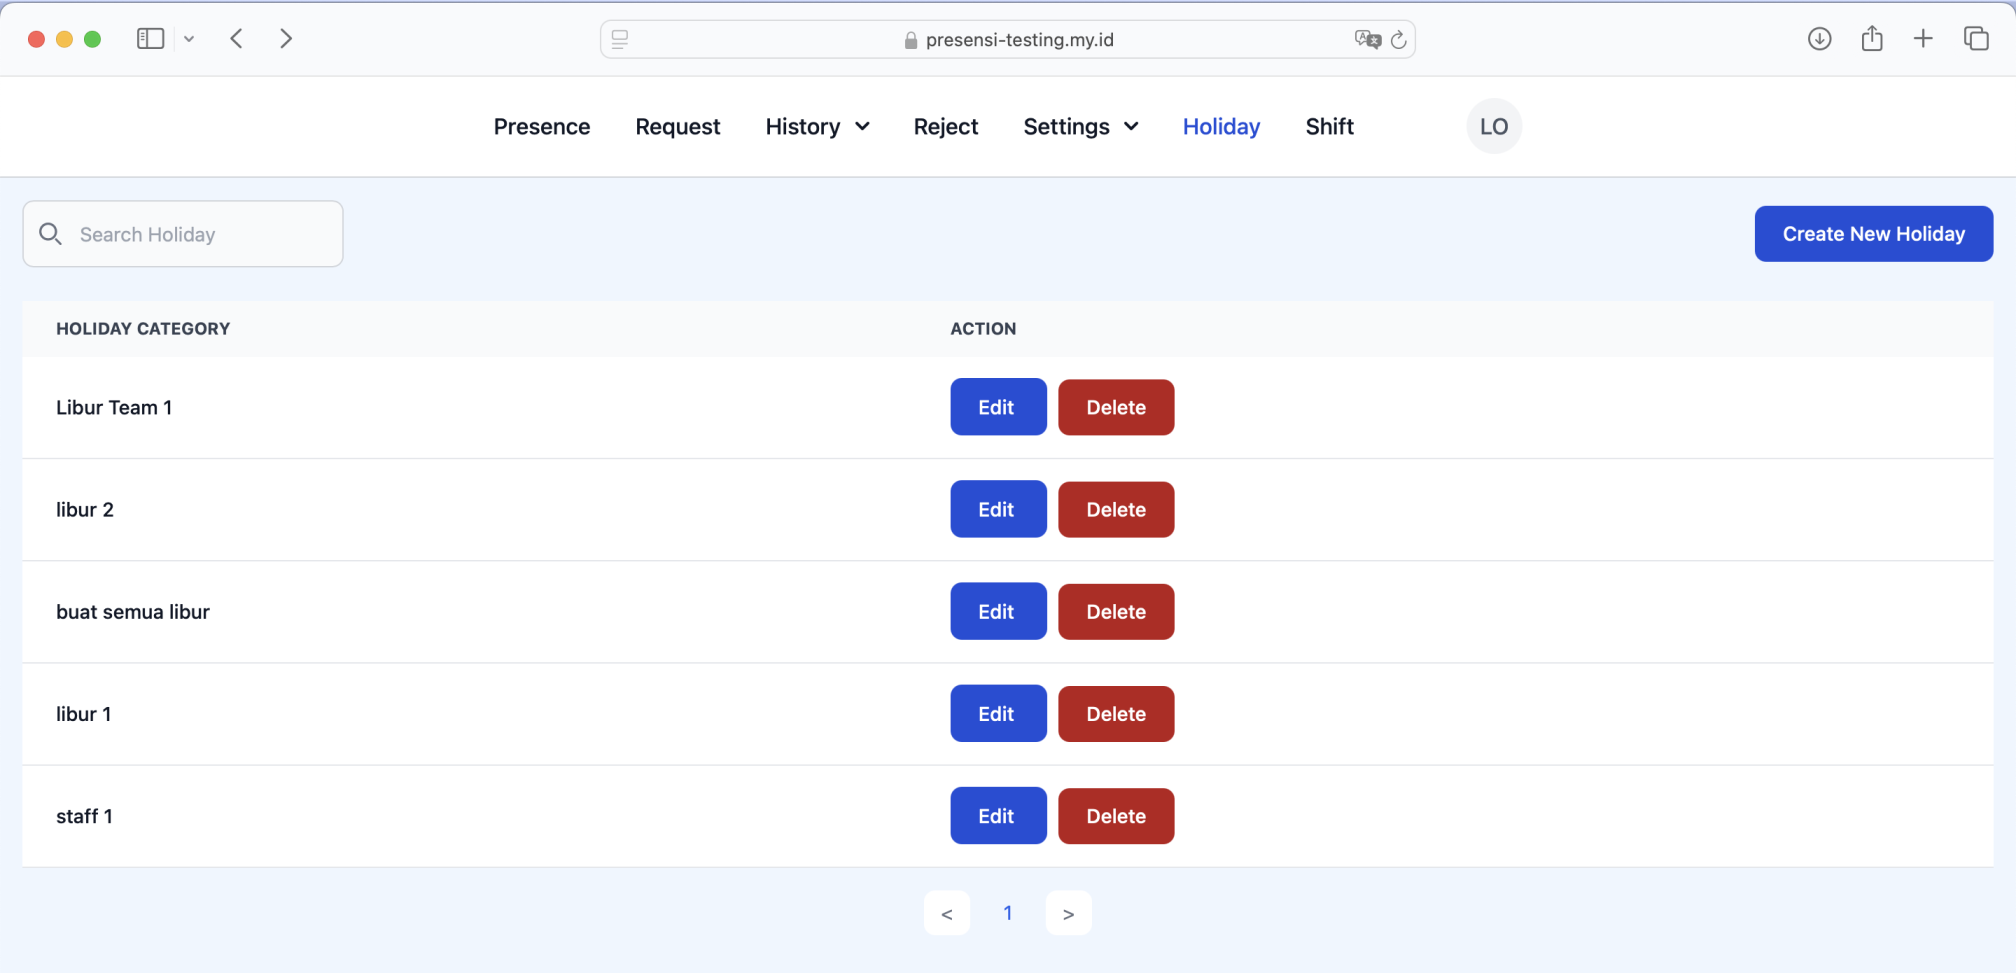
\includegraphics[width=8cm]{Gambar/bab3/user-manual/user-manual-halaman-jenis-libur-perusahaan.png}
    	\caption{Halaman \textit{Holiday}}
    	\label{fig:user-manual-halaman-holiday}
        \end{figure}
        \FloatBarrier
    \end{enumerate}

    \item Menambah Jenis Libur Perusahaan
    \begin{enumerate}
        \item Membuka halaman jenis libur perusahaan yang terdapat pada \textbf{Manual \ref{item:mengakses-jenis-libur-perusahaan}}.
        \item Menekan tombol "\textit{Create New Holiday}" pada halaman \textit{holiday}. \textbf{\ref{fig:user-manual-tombol-create-new-holiday}} menunjukkan tombol "\textit{Create New Holiday}" pada halaman \textit{holiday}.
        \begin{figure}[!htbp]
    	\centering
    	
\includegraphics[width=8cm]{Gambar/bab3/user-manual/user-manual-tombol-create-new-holiday.png}
    	\caption{Tombol "\textit{Create New Holiday}"}
    	\label{fig:user-manual-tombol-create-new-holiday}
        \end{figure}
        \FloatBarrier

        \item Mengisi seluruh \textit{input form} pada modal \textit{create new holiday}, kemudian tekan tombol "\textit{Create New Holiday Category}" untuk menyimpan data jenis libur perusahaan baru. \textbf{\ref{fig:user-manual-modal-create-new-holiday}} menunjukkan modal \textit{create new holiday}.
        \begin{figure}[!htbp]
    	\centering
    	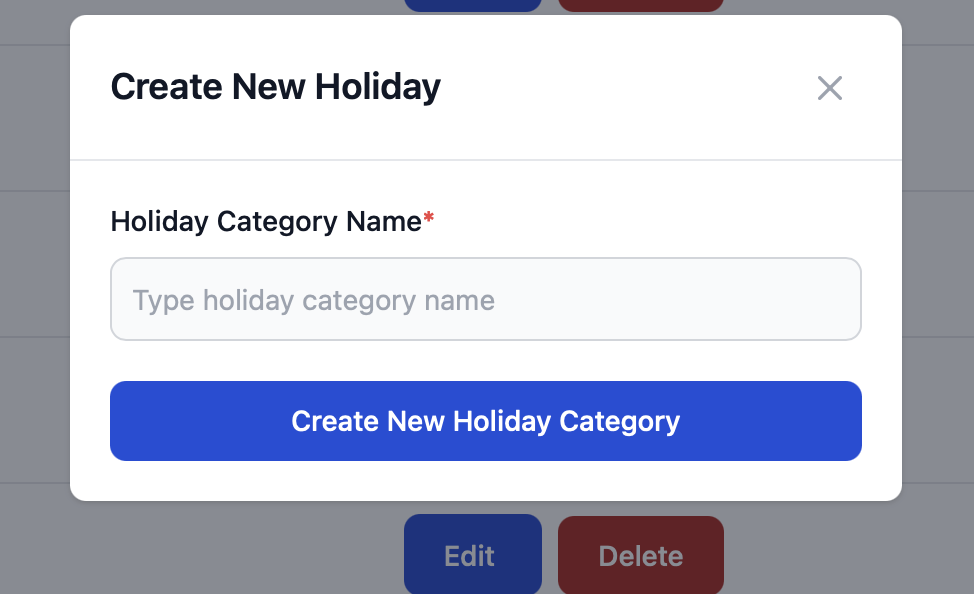
\includegraphics[width=8cm]{Gambar/bab3/user-manual/user-manual-modal-create-new-holiday.png}
    	\caption{Modal \textit{Create New Holiday}}
    	\label{fig:user-manual-modal-create-new-holiday}
        \end{figure}
        \FloatBarrier
    \end{enumerate}

    \item Menghapus Data Jenis Libur Perusahaan
    \begin{enumerate}
        \item Membuka halaman jenis libur perusahaan yang terdapat pada \textbf{Manual \ref{item:mengakses-jenis-libur-perusahaan}}.
        \item Menekan tombol "\textit{Delete}" pada salah satu data \textit{holiday} dan lakukan konfirmasi penghapusan. \textbf{\ref{fig:user-manual-tombol-delete-holiday}} menunjukkan tombol "\textit{Delete}" untuk menghapus data \textit{holiday}.
        \begin{figure}[!htbp]
    	\centering
    	
\includegraphics[width=8cm]{Gambar/bab3/user-manual/user-manual-tombol-delete-holiday.png}
    	\caption{Tombol \textit{Delete Holiday}}
    	\label{fig:user-manual-tombol-delete-holiday}
        \end{figure}
        \FloatBarrier
    \end{enumerate}

    \item Mengakses Halaman Hari Pada Jenis Libur Perusahaan\label{item:mengakses-halaman-hari-jenis-libur-perusahaan}
    \begin{enumerate}
        \item Membuka halaman jenis libur perusahaan yang terdapat pada \textbf{Manual \ref{item:mengakses-jenis-libur-perusahaan}}.
        \item Menekan tombol "\textit{Edit}" salah satu data \textit{holiday} pada halaman \textit{holiday}. \textbf{\ref{fig:user-manual-tombol-edit-holiday}} menunjukkan tombol "\textit{Edit}" pada halaman \textit{holiday}.
        \begin{figure}[!htbp]
    	\centering
    	
\includegraphics[width=8cm]{Gambar/bab3/user-manual/user-manual-tombol-edit-holiday.png}
    	\caption{Tombol \textit{Edit} \textit{Holiday}}
    	\label{fig:user-manual-tombol-edit-holiday}
        \end{figure}
        \FloatBarrier

        \item Sistem akan menampilkan halaman data hari pada jenis perusahaan yang dipilih. \textbf{\ref{fig:user-manual-halaman-hari-jenis-libur-perusahaan}} menunjukkan halaman hari pada jenis libur perusahaan.
        \begin{figure}[!htbp]
    	\centering
    	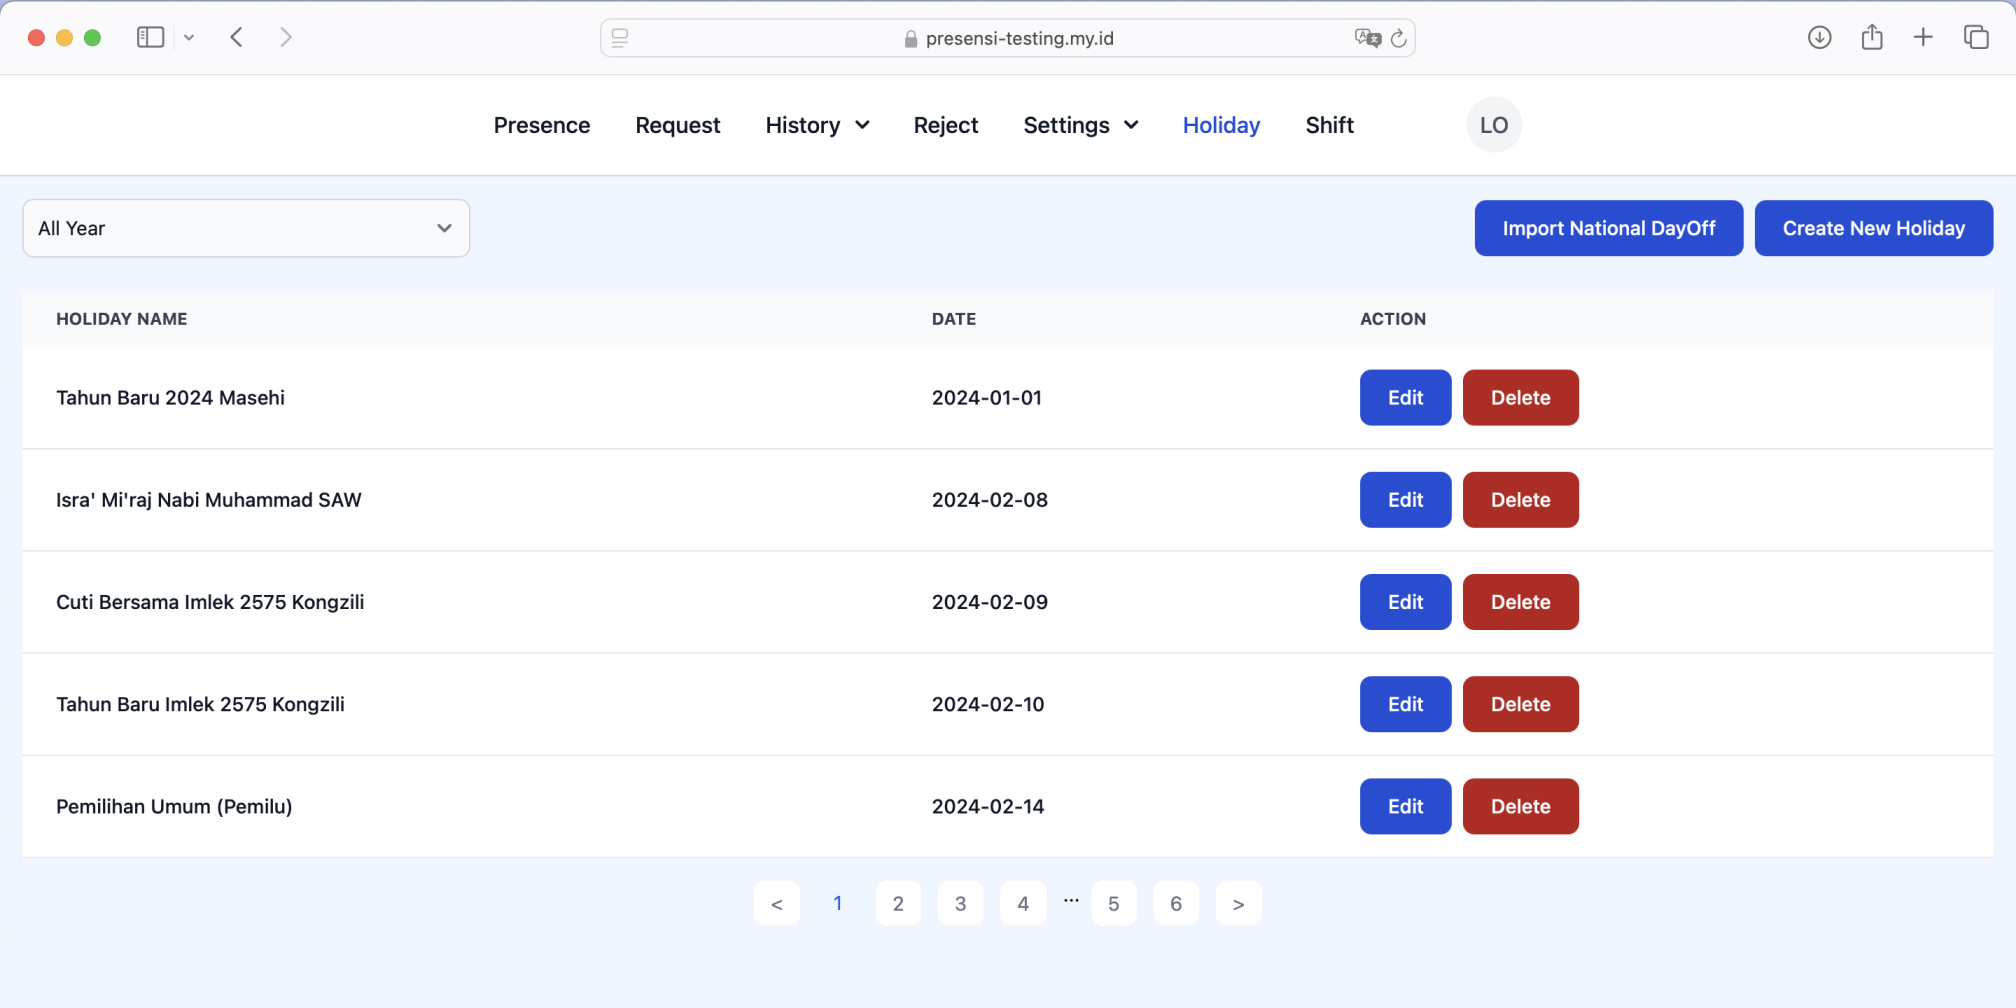
\includegraphics[width=8cm]{Gambar/bab3/user-manual/user-manual-halaman-hari-jenis-libur-perusahaan.png}
    	\caption{Halaman Hari Pada Jenis Libur Perusahaan}
    	\label{fig:user-manual-halaman-hari-jenis-libur-perusahaan}
        \end{figure}
        \FloatBarrier
    \end{enumerate}

    \item Menambah Hari Pada Jenis Libur Perusahaan
    \begin{enumerate}
        \item Membuka halaman pengaturan \textit{department} yang terdapat pada \textbf{Manual \ref{item:mengakses-halaman-hari-jenis-libur-perusahaan}}.
        \item Menekan tombol "\textit{Create New Holiday}" pada halaman hari pada jenis libur perusahaan. \textbf{\ref{fig:user-manual-tombol-tambah-hari-jenis-libur-perusahaan}} menunjukkan tombol "\textit{Create New Holiday}" pada halaman hari pada jenis libur perusahaan.
        \begin{figure}[!htbp]
    	\centering
    	
\includegraphics[width=8cm]{Gambar/bab3/user-manual/user-manual-tombol-tambah-hari-jenis-libur-perusahaan.png}
    	\caption{Tombol "\textit{Create New Holiday}"}
    	\label{fig:user-manual-tombol-tambah-hari-jenis-libur-perusahaan}
        \end{figure}
        \FloatBarrier

        \item Mengisi seluruh \textit{input form} pada modal \textit{create new holiday}, kemudian tekan tombol "\textit{Create New Holiday Category}" untuk menyimpan data hari pada jenis libur perusahaan. \textbf{\ref{fig:user-manual-modal-tambah-hari-pada-jenis-libur-perusahaan}} menunjukkan modal \textit{create new holiday}.
        \begin{figure}[!htbp]
    	\centering
    	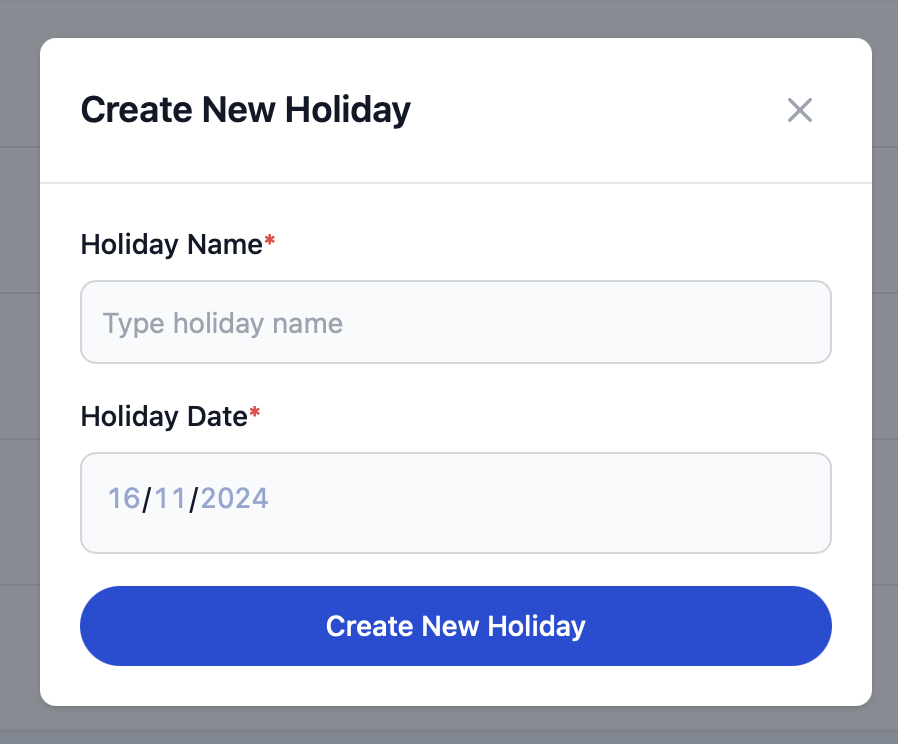
\includegraphics[width=8cm]{Gambar/bab3/user-manual/user-manual-modal-tambah-hari-jenis-libur-perusahaan.png}
    	\caption{Modal \textit{Create New Holiday}}
    	\label{fig:user-manual-modal-tambah-hari-pada-jenis-libur-perusahaan}
        \end{figure}
        \FloatBarrier
    \end{enumerate}


    \item Mengubah Data Hari Pada Jenis Libur Perusahaan
    \begin{enumerate}
        \item Membuka halaman hari pada jenis libur perusahaan yang terdapat pada \textbf{Manual \ref{item:mengakses-halaman-hari-jenis-libur-perusahaan}}.
        \item Menekan tombol "\textit{Edit}" salah satu data hari pada jenis libur perusahaan pada halaman hari jenis libur perusahaan. \textbf{\ref{fig:user-manual-tombol-edit-hari-jenis-libur-perusahaan}} menunjukkan tombol "\textit{Edit}" pada halaman hari jenis libur perusahaan.
        \begin{figure}[!htbp]
    	\centering
    	
\includegraphics[width=8cm]{Gambar/bab3/user-manual/user-manual-tombol-edit-hari-jenis-libur-perusahaan.png}
    	\caption{Tombol \textit{Edit} Pada Jenis Libur Perusahaan}
    	\label{fig:user-manual-tombol-edit-hari-jenis-libur-perusahaan}
        \end{figure}
        \FloatBarrier

        \item Mengubah seluruh \textit{input form} pada modal \textit{edit} hari jenis libur perusahaan, kemudian tekan tombol "\textit{Save Changes}" untuk menyimpan data hari pada jenis libur perusahaan. \textbf{\ref{fig:user-manual-modal-edit-hari-jenis-libur-perusahaan}} menunjukkan modal \textit{edit} hari jenis libur perusahaan.
        \begin{figure}[!htbp]
    	\centering
    	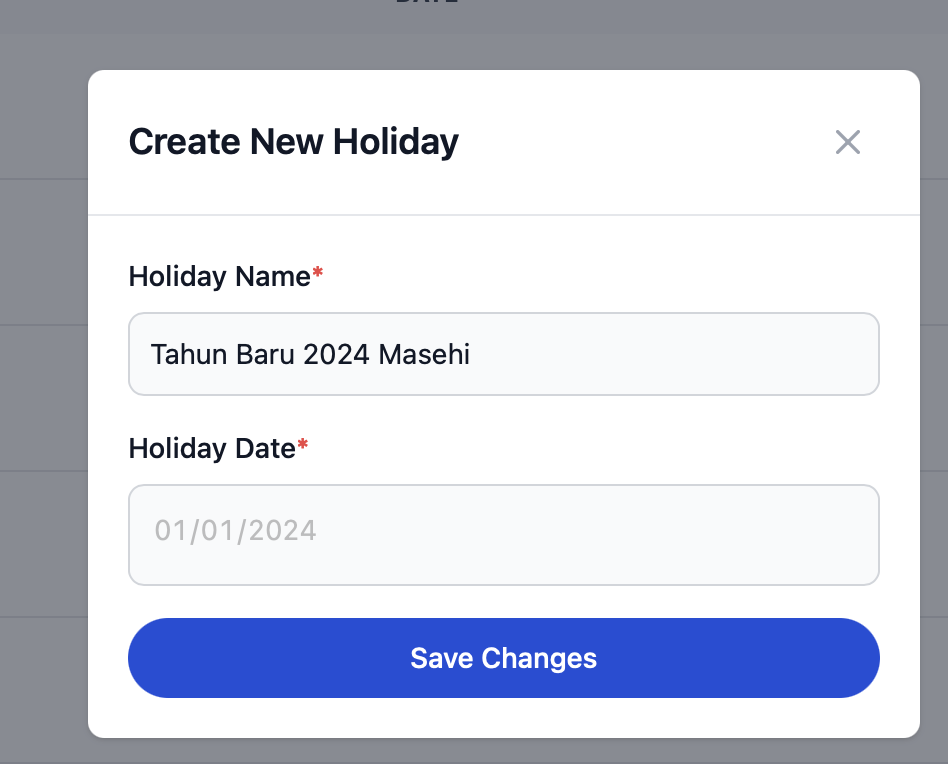
\includegraphics[width=8cm]{Gambar/bab3/user-manual/user-manual-modal-edit-hari-jenis-libur-perusahaan.png}
    	\caption{Modal \textit{Edit} Hari Pada Jenis Libur Perusahaan}
    	\label{fig:user-manual-modal-edit-hari-jenis-libur-perusahaan}
        \end{figure}
        \FloatBarrier
    \end{enumerate}

    \item Menghapus Data Hari Pada Jenis Libur Perusahaan
    \begin{enumerate}
        \item Membuka halaman hari pada jenis libur perusahaan yang terdapat pada \textbf{Manual \ref{item:mengakses-halaman-hari-jenis-libur-perusahaan}}.
        \item Menekan tombol "\textit{Delete}" pada salah satu data hari pada jenis libur perusahaan dan lakukan konfirmasi penghapusan. \textbf{\ref{fig:user-manual-tombol-delete-hari-jenis-libur-perusahaan}} menunjukkan tombol "\textit{Delete}" untuk menghapus data hari pada jenis libur perusahaan.
        \begin{figure}[!htbp]
    	\centering
    	
\includegraphics[width=8cm]{Gambar/bab3/user-manual/user-manual-hapus-hari-jenis-libur-perusahaan.png}
    	\caption{Tombol \textit{Delete} Hari Pada Jenis Libur Perusahaan}
    	\label{fig:user-manual-tombol-delete-hari-jenis-libur-perusahaan}
        \end{figure}
        \FloatBarrier
    \end{enumerate}

    \item Mengimpor Hari Libur Nasional Otomatis Pada Jenis Libur Perusahaan
    \begin{enumerate}
        \item Membuka halaman hari pada jenis libur perusahaan yang terdapat pada \textbf{Manual \ref{item:mengakses-halaman-hari-jenis-libur-perusahaan}}.
        \item Menekan tombol "\textit{Import National DayOff}" pada halaman hari jenis libur perusahaan. \textbf{\ref{fig:user-manual-tombol-import-libur-nasional-hari-jenis-libur-perusahaan}} menunjukkan tombol "\textit{Import National DayOff}" untuk mengambil data libur nasional Indonesia secara otomatis.
        \begin{figure}[!htbp]
    	\centering
    	
\includegraphics[width=8cm]{Gambar/bab3/user-manual/user-manual-tombol-import-hari-libur-nasional.png}
    	\caption{Tombol \textit{Import} Hari Libur Nasional Pada Jenis Libur Perusahaan}
    	\label{fig:user-manual-tombol-import-libur-nasional-hari-jenis-libur-perusahaan}
        \end{figure}
        \FloatBarrier
        \item Memilih tahun yang akan dicari hari liburnya dan menekan tombol "\textit{Add}" untuk melihat \textit{preview} data libur nasional Indonesia, pilih data yang ingin dimasukkan kemudian tekan tombol "\textit{Import Now}" pada modal \textit{import national DayOff}. \textbf{\ref{fig:user-manual-modal-import-libur-nasional-hari-jenis-libur-perusahaan}} menunjukkan modal \textit{import national DayOff}.
        \begin{figure}[!htbp]
    	\centering
    	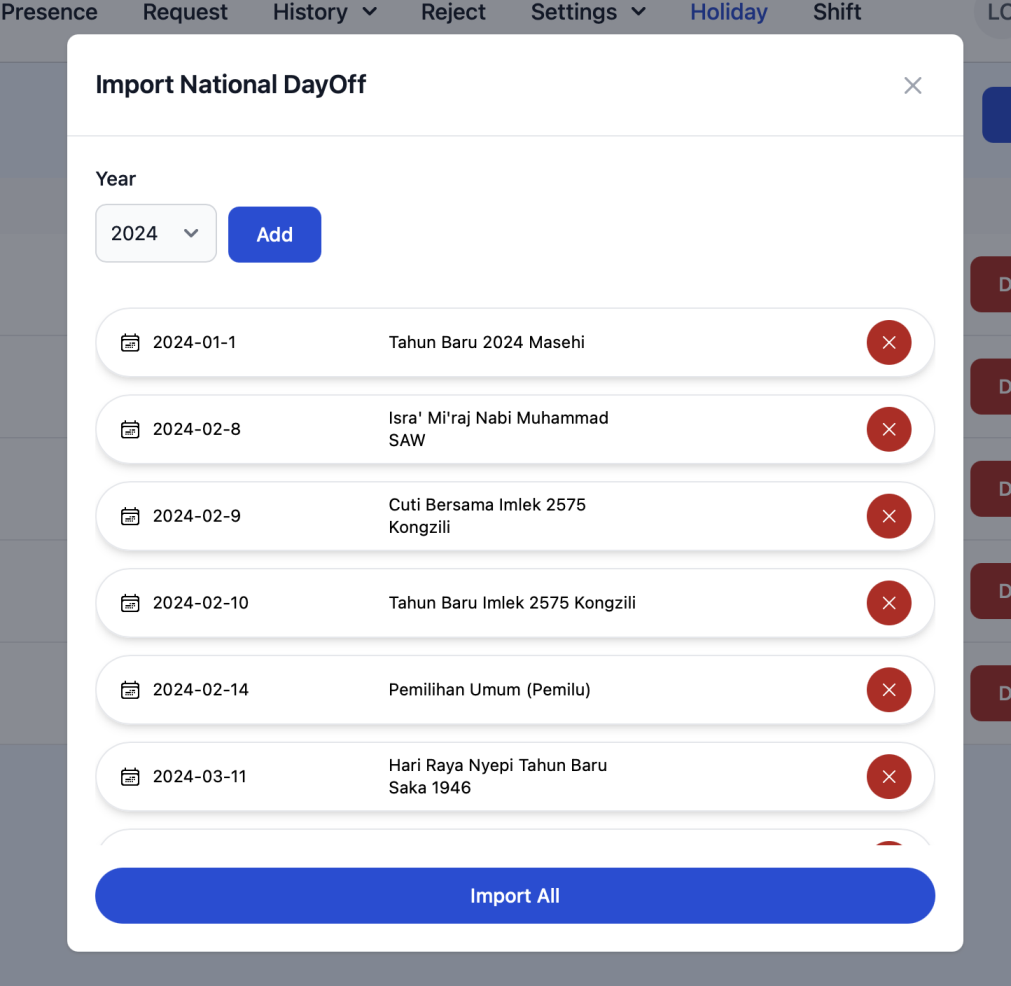
\includegraphics[width=8cm]{Gambar/bab3/user-manual/user-manual-modal-import-hari-libur-nasional.png}
    	\caption{Modal \textit{Import} Hari Libur Nasional Pada Jenis Libur Perusahaan}
    	\label{fig:user-manual-modal-import-libur-nasional-hari-jenis-libur-perusahaan}
        \end{figure}
        \FloatBarrier

         \item Sistem akan menampilkan modal untuk memberikan informasi terkait data yang berhasil di\textit{import} dan gagal. \textbf{\ref{fig:user-manual-modal-hasil-import-libur-nasional-hari-jenis-libur-perusahaan}} menunjukkan hasil \textit{import} data hari libur nasional Indonesia.
    \begin{figure}[!htbp]
    	\centering
    	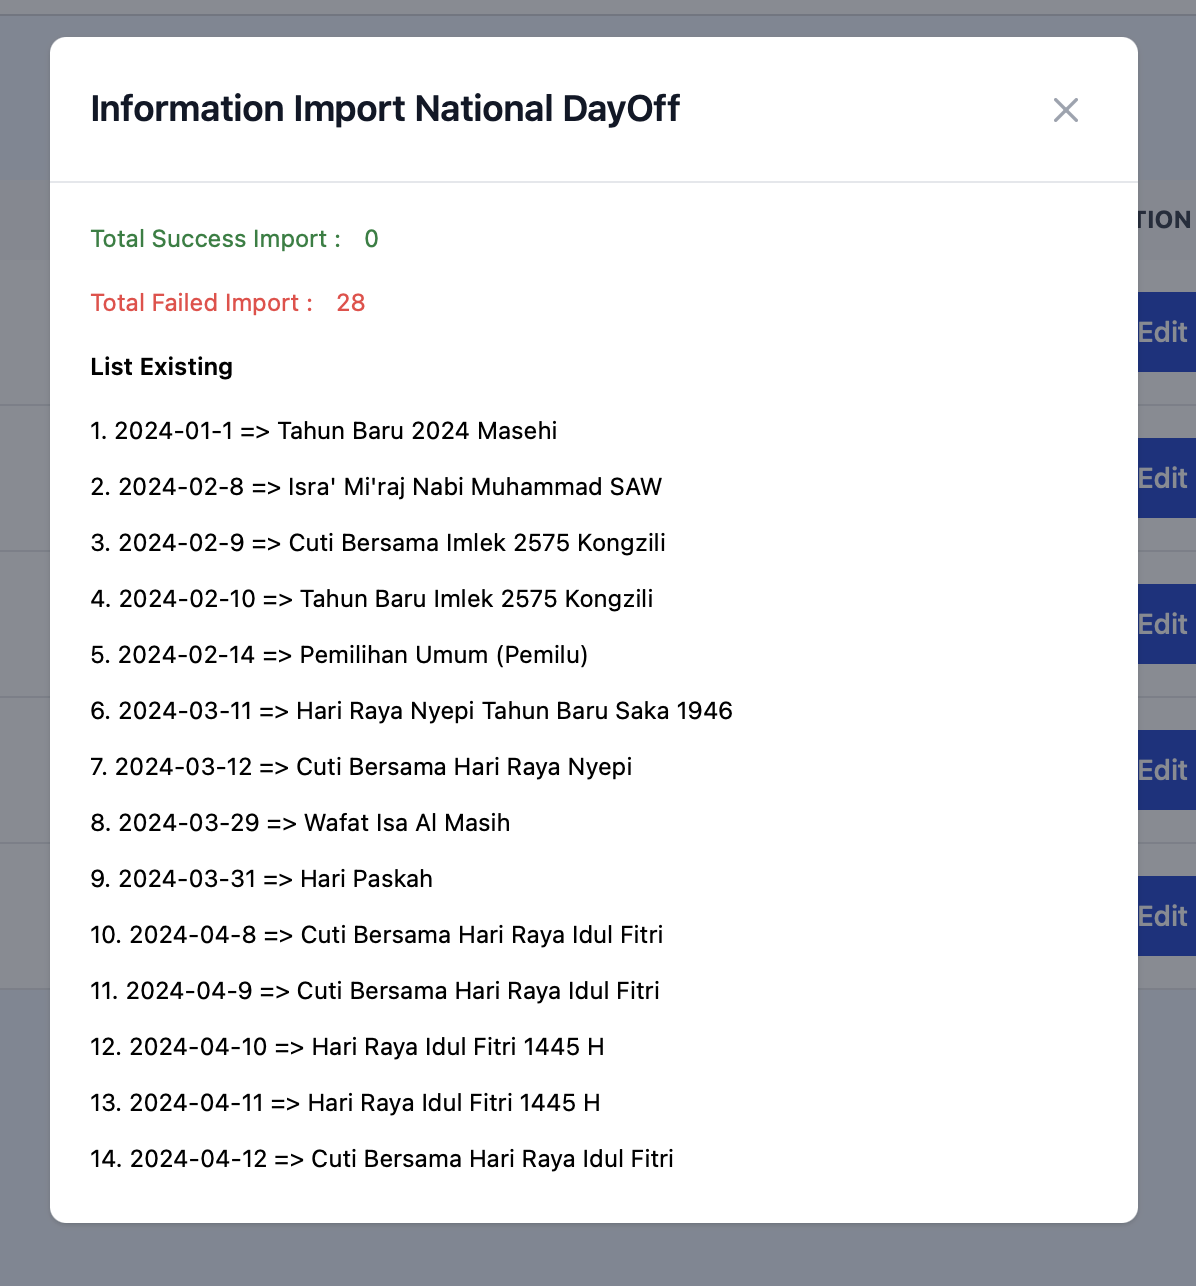
\includegraphics[width=8cm]{Gambar/bab3/user-manual/user-manual-modal-hasil-import-hari-libur-nasional.png}
    	\caption{Modal Hasil \textit{Import} Hari Libur Nasional Pada Jenis Libur Perusahaan}
    	\label{fig:user-manual-modal-hasil-import-libur-nasional-hari-jenis-libur-perusahaan}
        \end{figure}
    \FloatBarrier
    \end{enumerate}

    % BELUM DI INSERT GAMBAR 

    \item Mengakses Halaman Jenis \textit{Shift}\label{item:mengakses-halaman-jenis-shift}
    \begin{enumerate}
        \item Melakukan \textit{login} pada aplikasi presensi \textit{online} yang terdapat pada \textbf{Manual \ref{item:melakukan-login}}.
        \item Menekan tombol "\textit{Shift}" pada \textit{navigation bar} yang terletak di paling atas. \textbf{\ref{fig:user-manual-tombol-shift-pada-navigation-bar}} menunjukkan tombol \textit{"Shift"} pada \textit{navigation bar}.
        \begin{figure}[!htbp]
    	\centering
    	
\includegraphics[width=8cm]{Gambar/bab3/user-manual/user-manual-navbar-shift.png}
    	\caption{Tombol \textit{Shift} Pada \textit{Navigation Bar}}
    	\label{fig:user-manual-tombol-shift-pada-navigation-bar}
        \end{figure}
        \FloatBarrier
        \item Sistem akan menampilkan halaman jenis \textit{shift} beserta data jenis \textit{shift}. \textbf{\ref{fig:user-manual-halaman-jenis-shift}} menunjukkan halaman jenis \textit{shift}.
        \begin{figure}[!htbp]
    	\centering
    	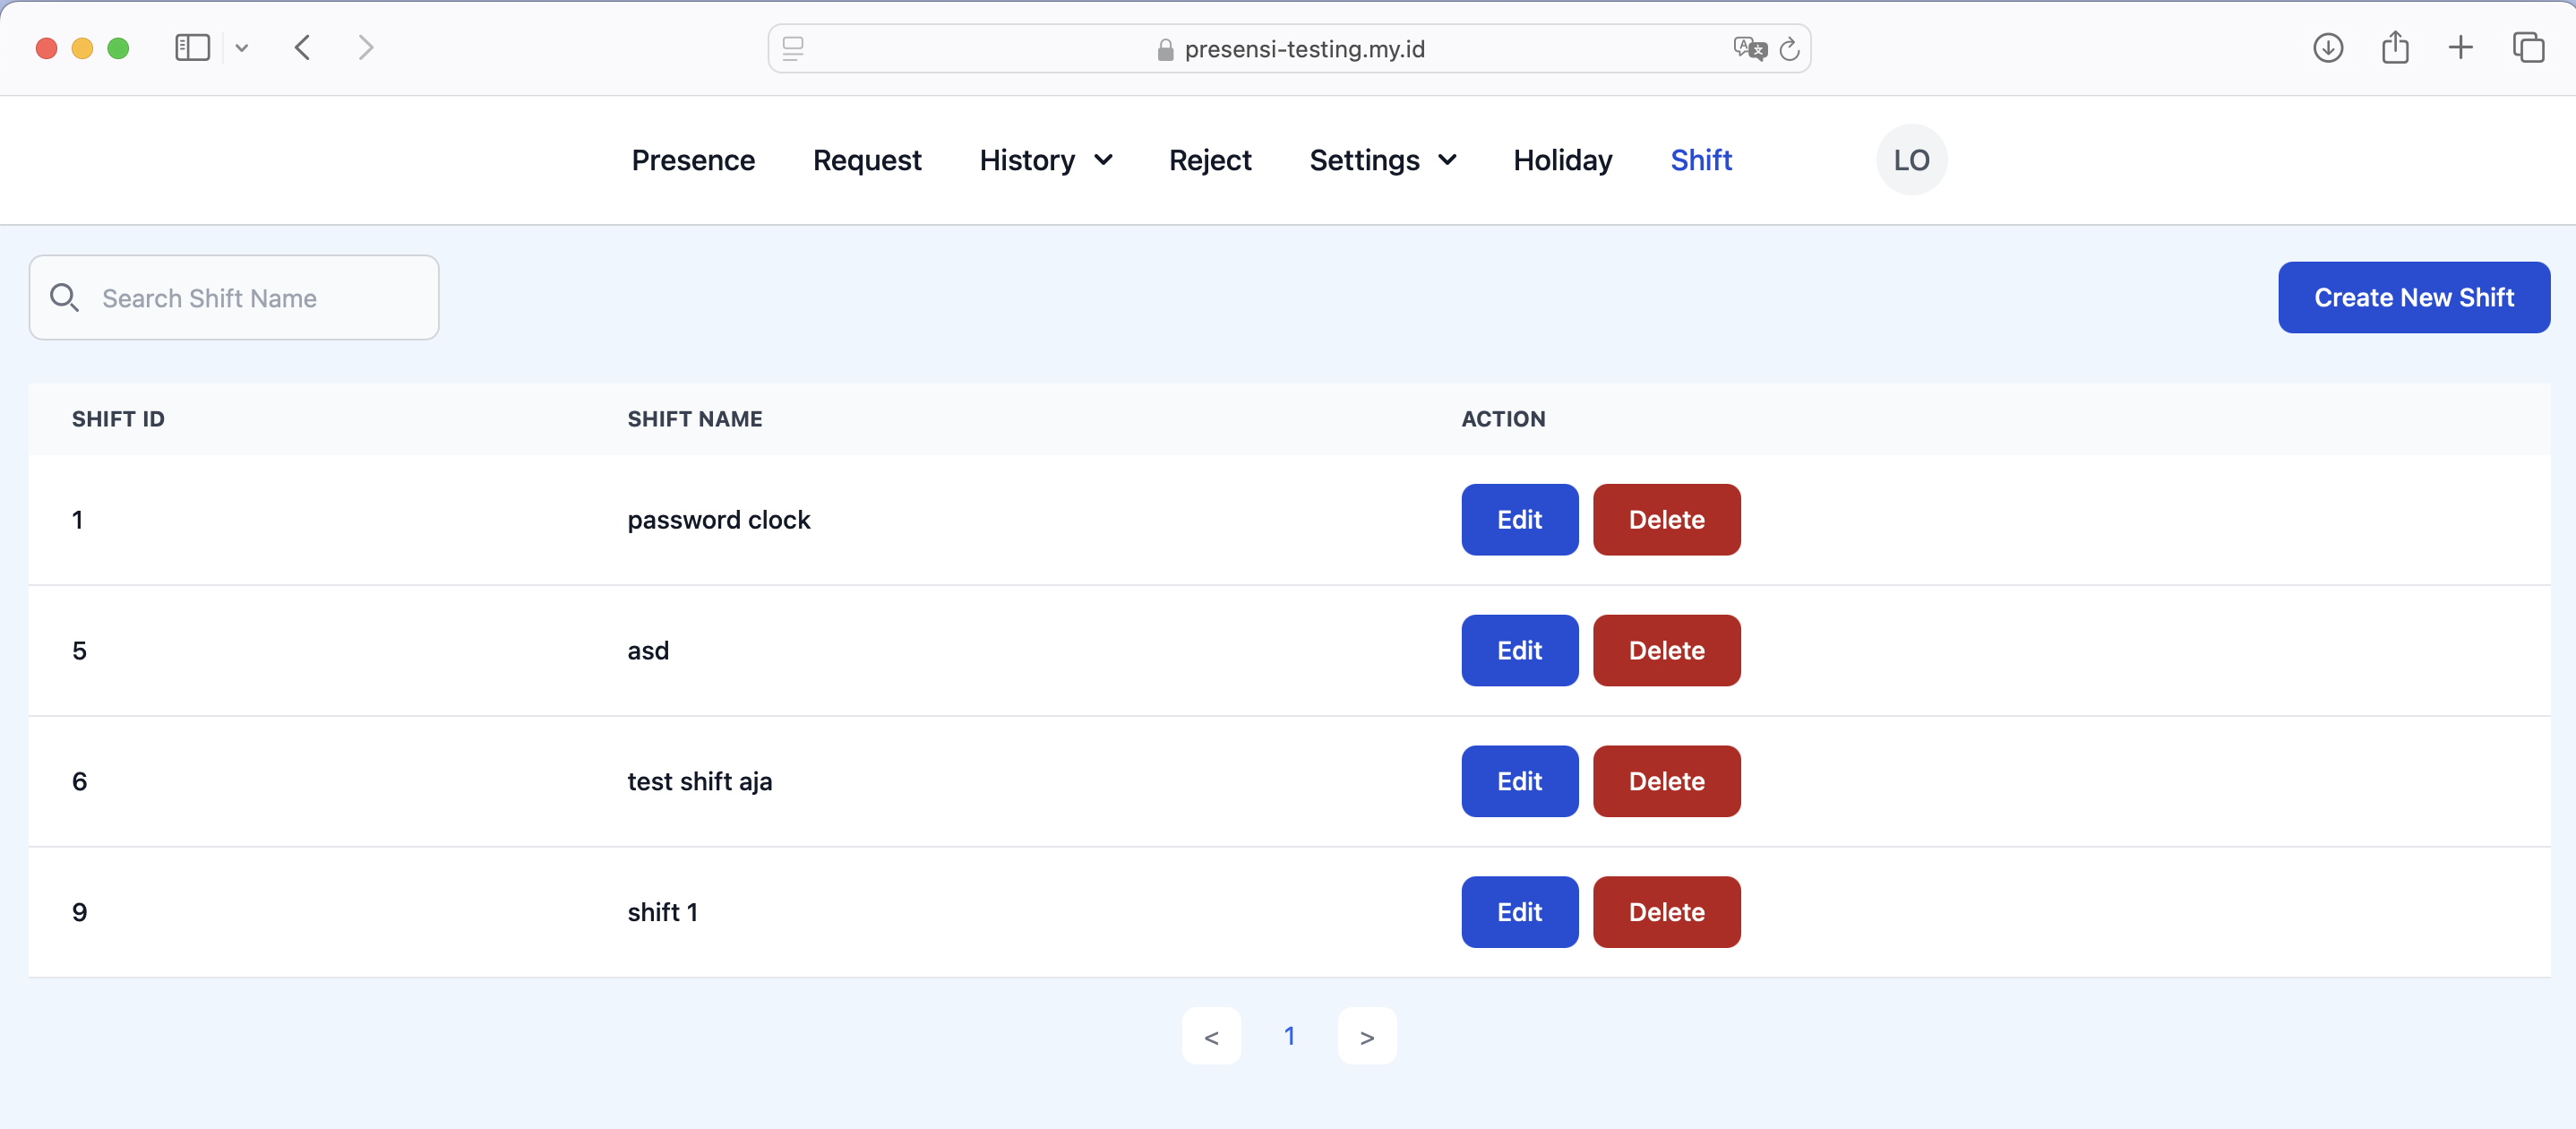
\includegraphics[width=8cm]{Gambar/bab3/user-manual/user-manual-halaman-jenis-shift.png}
    	\caption{Halaman Jenis \textit{Shift}}
    	\label{fig:user-manual-halaman-jenis-shift}
        \end{figure}
        \FloatBarrier
    \end{enumerate}

    \item Menambah Jenis \textit{Shift}
    \begin{enumerate}
        \item Membuka halaman jenis libur \textit{shift} yang terdapat pada \textbf{Manual \ref{item:mengakses-halaman-jenis-shift}}.
        \item Menekan tombol "\textit{Create New Shift}" pada halaman jenis \textit{shift}. \textbf{\ref{fig:user-manual-tombol-create-new-shift}} menunjukkan tombol "\textit{Create New Shift}" pada halaman jenis \textit{shift}.
        \begin{figure}[!htbp]
    	\centering
    	
\includegraphics[width=8cm]{Gambar/bab3/user-manual/user-manual-tombol-create-new-shift.png}
    	\caption{Tombol \textit{Create New Shift} Pada Halaman Jenis \textit{Shift}}
    	\label{fig:user-manual-tombol-create-new-shift}
        \end{figure}
        \FloatBarrier
        \item Mengisi seluruh \textit{input form} pada modal \textit{create new shift} dan tekan tombol \textit{"Create New Shift"} untuk menyimpan data jenis \textit{shift} baru. \textbf{\ref{fig:user-manual-modal-create-new-shift}} menunjukkan modal \textit{create new shift}.
        \begin{figure}[!htbp]
    	\centering
    	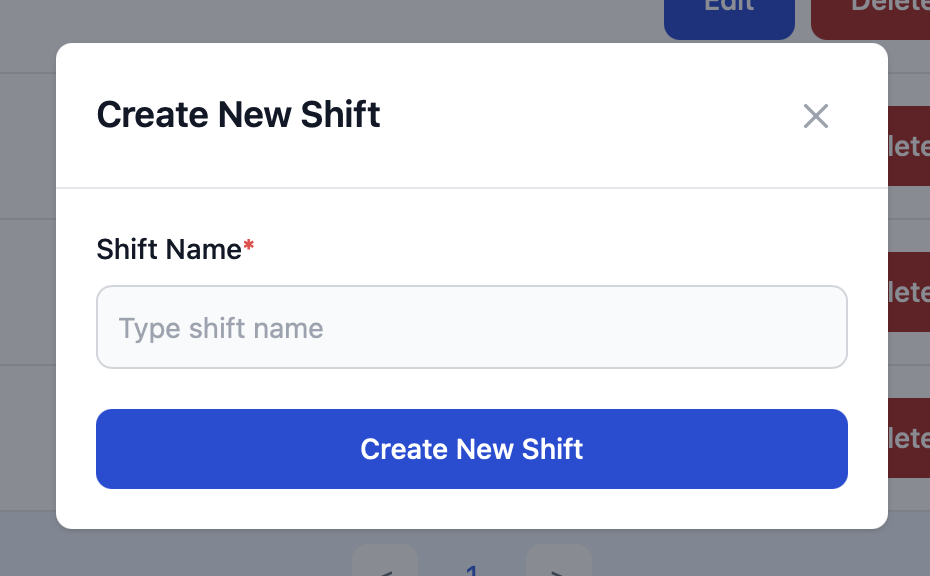
\includegraphics[width=8cm]{Gambar/bab3/user-manual/user-manual-modal-create-new-shift.png}
    	\caption{Modal \textit{Create New Shift} Pada Halaman Jenis \textit{Shift}}
    	\label{fig:user-manual-modal-create-new-shift}
        \end{figure}
        \FloatBarrier
    \end{enumerate}

    \item Menghapus Jenis \textit{Shift}
    \begin{enumerate}
        \item Membuka halaman jenis libur \textit{shift} yang terdapat pada \textbf{Manual \ref{item:mengakses-halaman-jenis-shift}}.
        \item Menekan tombol "\textit{Delete}" pada salah satu data jenis \textit{shift} melalui halaman jenis \textit{shift} dan melakukan konfirmasi. \textbf{\ref{fig:user-manual-tombol-delete-shift}} menunjukkan tombol "\textit{Delete}" pada salah satu data jenis \textit{shift}.
        \begin{figure}[!htbp]
    	\centering
    	
\includegraphics[width=5cm]{Gambar/bab3/user-manual/user-manual-tombol-delete-shift.png}
    	\caption{Tombol \textit{Delete} Pada Jenis \textit{Shift}}
    	\label{fig:user-manual-tombol-delete-shift}
        \end{figure}
        \FloatBarrier
    \end{enumerate}

    \item Melakukan \textit{Edit} Jenis \textit{Shift}\label{item:melakukan-edit-jenis-shift}
    \begin{enumerate}
        \item Membuka halaman jenis libur \textit{shift} yang terdapat pada \textbf{Manual \ref{item:mengakses-halaman-jenis-shift}}.
        \item Menekan tombol "\textit{Edit}" pada salah satu data jenis \textit{shift} melalui halaman jenis \textit{shift}. \textbf{\ref{fig:user-manual-tombol-edit-shift}} menunjukkan tombol "\textit{Edit}" pada salah satu data jenis \textit{shift}.
        \begin{figure}[!htbp]
    	\centering
    	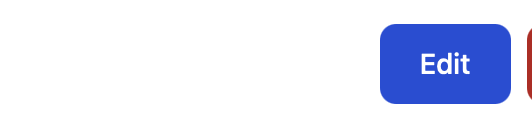
\includegraphics[width=5cm]{Gambar/bab3/user-manual/user-manual-tombol-edit-shift.png}
    	\caption{Tombol \textit{Edit} Pada Jenis \textit{Shift}}
    	\label{fig:user-manual-tombol-edit-shift}
        \end{figure}
        \FloatBarrier
        
        \item Mengisi \textit{input form} pada modal \textit{edit shift} dan tekan tombol "\textit{Save Changes}" untuk menyimpan perubahan jenis \textit{shift}. \textbf{\ref{fig:user-manual-tombol-edit-jenis-shift}} menunjukkan modal \textit{edit shift}.
        \begin{figure}[!htbp]
    	\centering
    	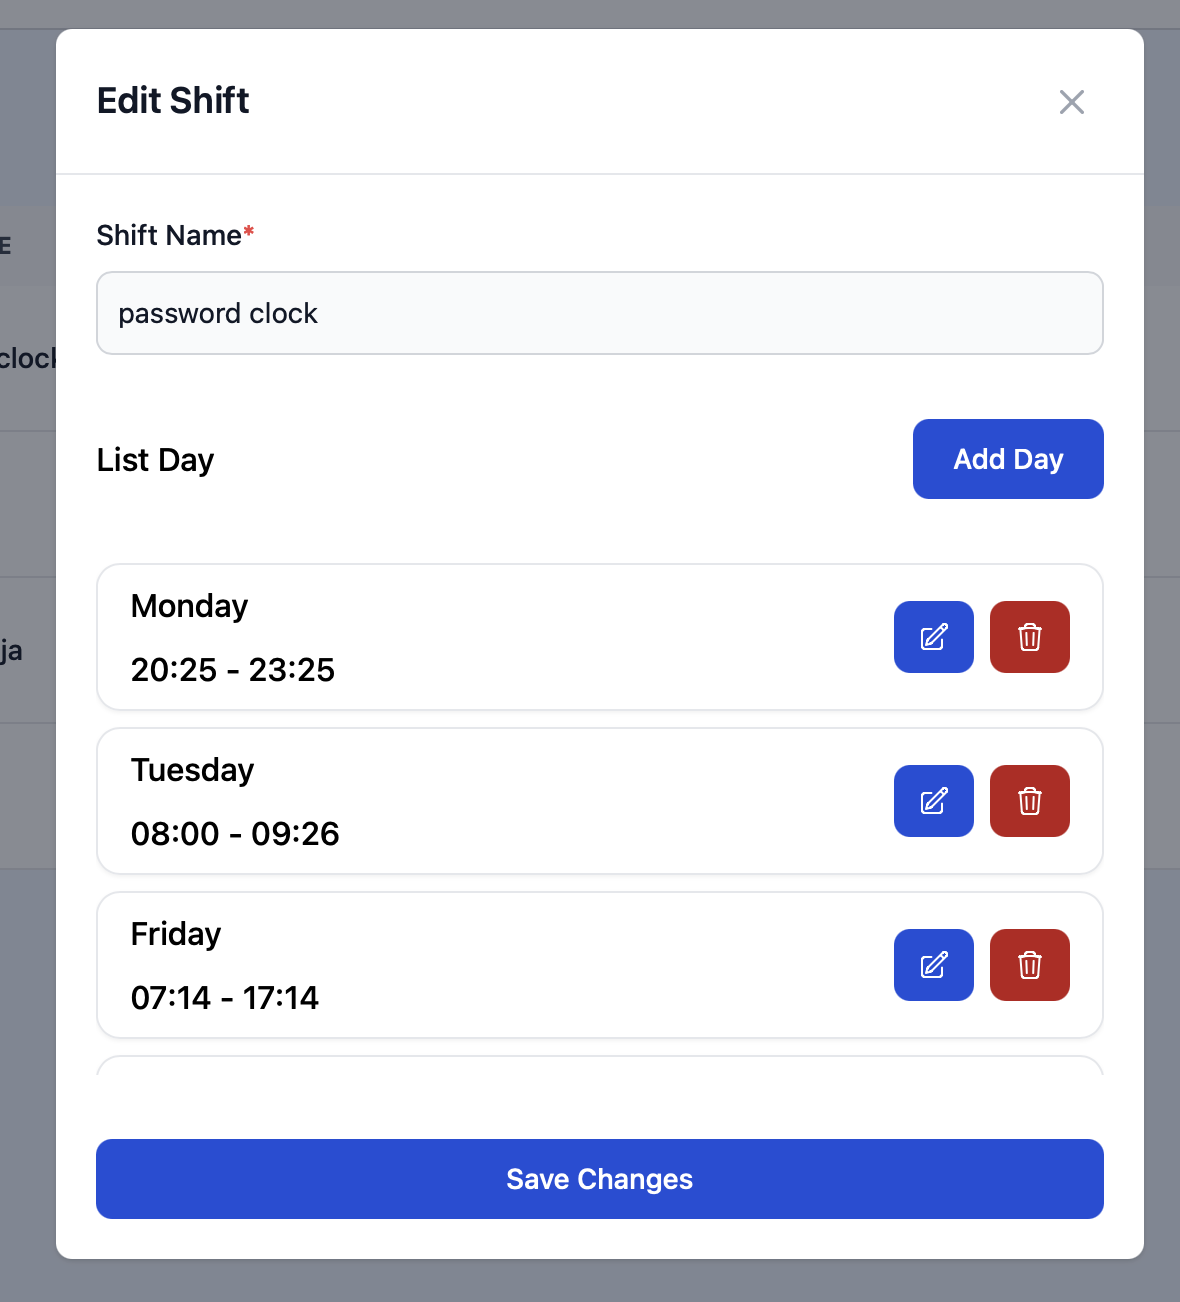
\includegraphics[width=8cm]{Gambar/bab3/user-manual/user-manual-modal-edit-shift.png}
    	\caption{Tombol \textit{Edit} Pada Jenis \textit{Shift}}
    	\label{fig:user-manual-tombol-edit-jenis-shift}
        \end{figure}
        \FloatBarrier
    \end{enumerate}

    \item Menambah Hari Pada Jenis \textit{Shift}
    \begin{enumerate}
        \item Mengakses modal \textit{edit} jenis \textit{shift} pada \textbf{Manual \ref{item:melakukan-edit-jenis-shift}}.
        \item Menekan tombol "\textit{Add Day}" pada modal \textit{edit} jenis \textit{shift}. \textbf{\ref{fig:user-manual-tombol-add-shift-day}} menunjukkan tombol \textit{"Add Day"} untuk membuka modal \textit{add shift day}.
        \begin{figure}[!htbp]
    	\centering
    	
\includegraphics[width=5cm]{Gambar/bab3/user-manual/user-manual-tombol-add-shiftday.png}
    	\caption{Tombol \textit{Add Day} Pada Jenis \textit{Shift}}
    	\label{fig:user-manual-tombol-add-shift-day}
        \end{figure}
        \FloatBarrier
        \item Mengisi seluruh \textit{input form} pada \textit{add shift day} dan menekan tombol "\textit{Add Day}" untuk menyimpan hari baru pada jenis \textit{shift}. \textbf{\ref{fig:user-manual-modal-add-shift-day}} menunjukkan modal \textit{add shift day} untuk menambah hari baru pada jenis \textit{shift}.
        \begin{figure}[!htbp]
    	\centering
    	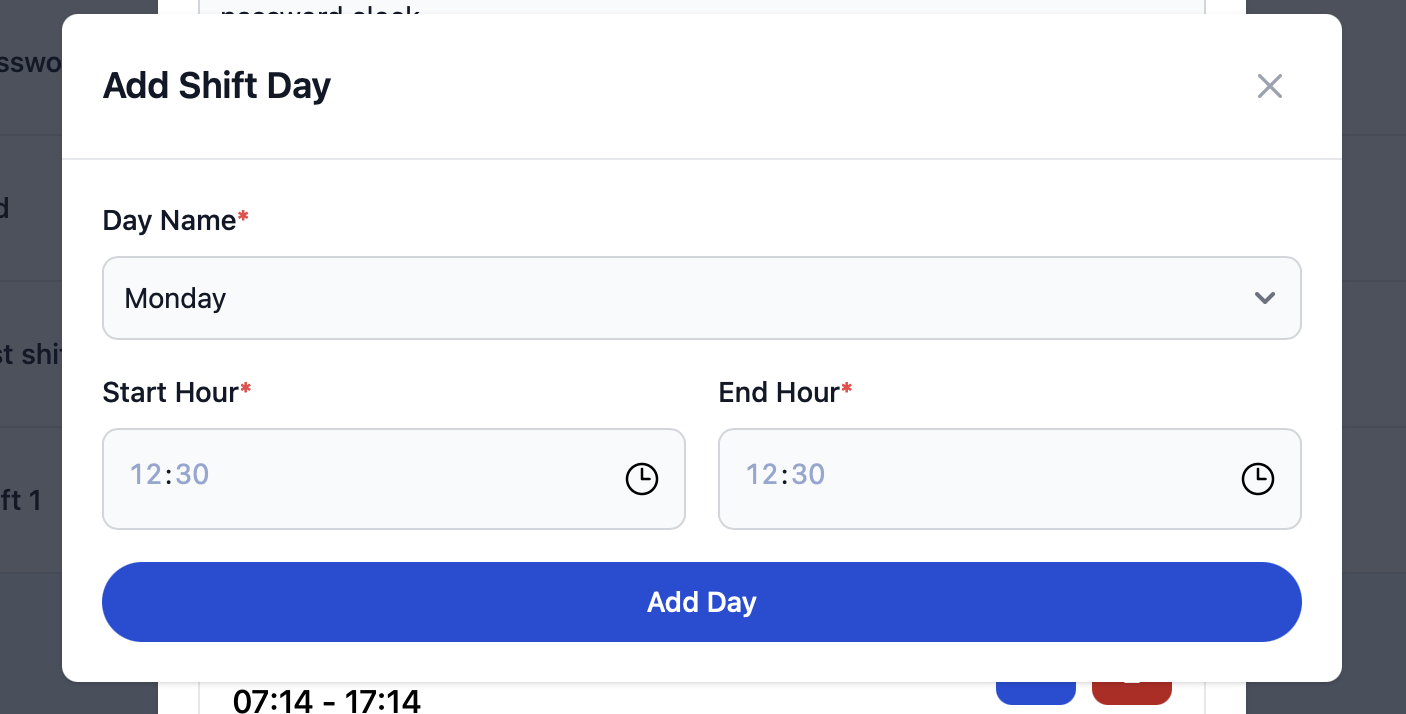
\includegraphics[width=8cm]{Gambar/bab3/user-manual/user-manual-modal-add-shiftday.png}
    	\caption{Modal \textit{Add New Day} Pada Jenis \textit{Shift}}
    	\label{fig:user-manual-modal-add-shift-day}
        \end{figure}
        \FloatBarrier
        
    \end{enumerate}

    \item Melakukan \textit{Edit} Hari Pada Jenis \textit{Shift}
    \begin{enumerate}
        \item Mengakses modal \textit{edit} jenis \textit{shift} pada \textbf{Manual \ref{item:melakukan-edit-jenis-shift}}.
        \item Menekan logo \textit{edit} salah satu hari pada modal \textit{edit} jenis \textit{shift}. \textbf{\ref{fig:user-manual-tombol-edit-shift-day}} menunjukkan tombol logo \textit{edit} untuk mengubah data hari pada jenis \textit{shift}.
        \begin{figure}[!htbp]
    	\centering
    	
\includegraphics[width=5cm]{Gambar/bab3/user-manual/user-manual-tombol-edit-shiftday.png}
    	\caption{Tombol \textit{Edit Day} Pada Jenis \textit{Shift}}
    	\label{fig:user-manual-tombol-edit-shift-day}
        \end{figure}
        \FloatBarrier
        \item Mengubah isi \textit{input form} pada modal \textit{edit shift day} dan menekan tombol \textit{"Edit Day"} untuk menyimpan perubahan data hari pada jenis \textit{shift}. \textbf{\ref{fig:user-manual-modal-edit-shift-day}} menunjukkan modal \textit{edit shift day} untuk mengubah data hari pada jenis \textit{shift}.
        \begin{figure}[!htbp]
    	\centering
    	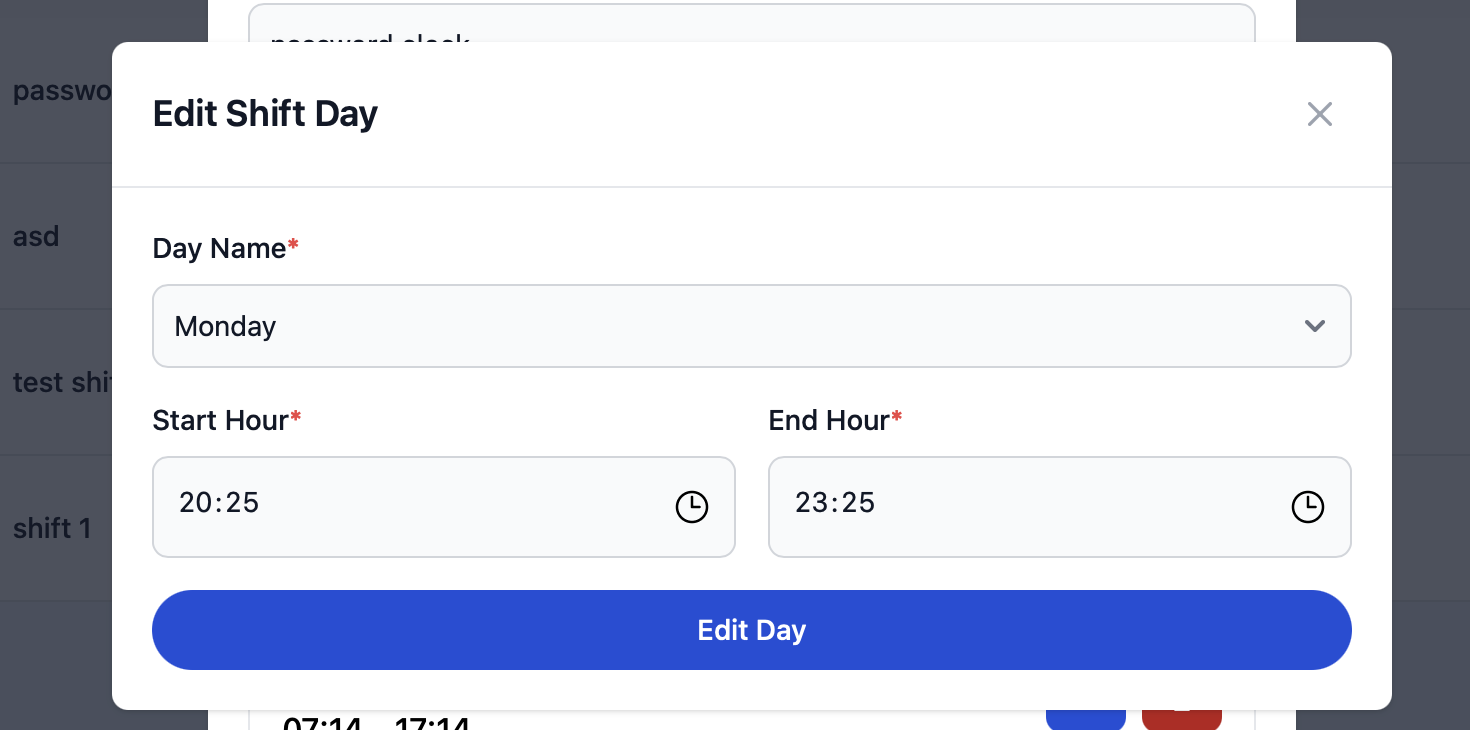
\includegraphics[width=8cm]{Gambar/bab3/user-manual/user-manual-modal-edit-shiftday.png}
    	\caption{Modal \textit{Edit Day} Pada Jenis \textit{Shift}}
    	\label{fig:user-manual-modal-edit-shift-day}
        \end{figure}
        \FloatBarrier
    \end{enumerate}

    \item Menghapus Hari Pada Jenis Shift
    \begin{enumerate}
        \item Mengakses modal \textit{edit} jenis \textit{shift} pada \textbf{Manual \ref{item:melakukan-edit-jenis-shift}}.
        \item Menekan tombol logo hapus salah satu data hari pada modal \textit{edit} jenis \textit{shift} dan melakukan konfirmasi penghapusan. \textbf{\ref{fig:user-manual-tombol-delete-shift-day}} menunjukkan tombol logo hapus salah satu data hari pada jenis \textit{shift}.
        \begin{figure}[!htbp]
    	\centering
    	
\includegraphics[width=5cm]{Gambar/bab3/user-manual/user-manual-tombol-delete-shiftday.png}
    	\caption{Tombol \textit{Delete} Hari Pada Jenis \textit{Shift}}
    	\label{fig:user-manual-tombol-delete-shift-day}
        \end{figure}
        \FloatBarrier
    \end{enumerate}

    \item Melakukan Ganti Kata Sandi Akun
    \begin{enumerate}
        \item Melakukan \textit{login} pada aplikasi presensi \textit{online} yang terdapat pada \textbf{Manual \ref{item:melakukan-login}}.
        \item Menekan ikon profil pada \textit{navigation bar} yang terletak di paling atas, kemudian memilih tombol "\textit{Change Password}". \textbf{\ref{fig:user-manual-tombol-change-password-pada-navigation-bar}} menunjukkan tombol \textit{"Change Password"} pada \textit{navigation bar}.
        \begin{figure}[!htbp]
    	\centering
    	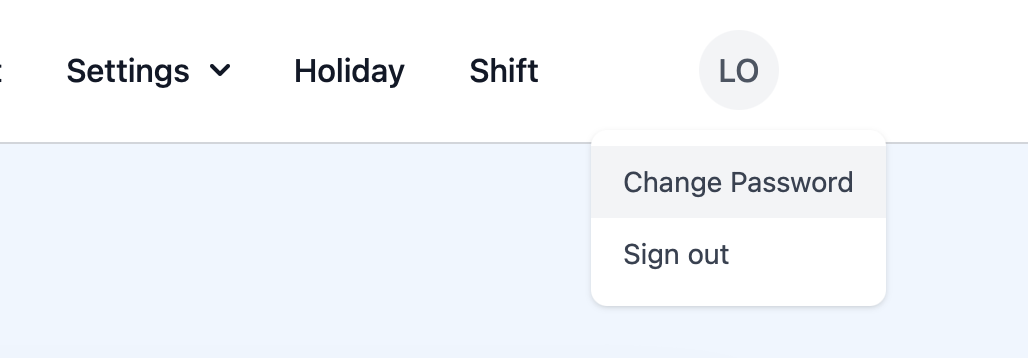
\includegraphics[width=8cm]{Gambar/bab3/user-manual/user-manual-navbar-change-password.png}
    	\caption{Tombol \textit{Change Password} Pada \textit{Navigation Bar}}
    	\label{fig:user-manual-tombol-change-password-pada-navigation-bar}
        \end{figure}
        \FloatBarrier
        \item Mengisi seluruh \textit{input form password} lama dan baru, kemudian tekan tombol "\textit{Submit}" untuk menyimpan perubahan \textit{password} baru pada akun. \textbf{\ref{fig:user-manual-halaman-change-password}} menunjukkan \textit{form} untuk pengubahan \textit{password} akun. 
        \begin{figure}[!htbp]
    	\centering
    	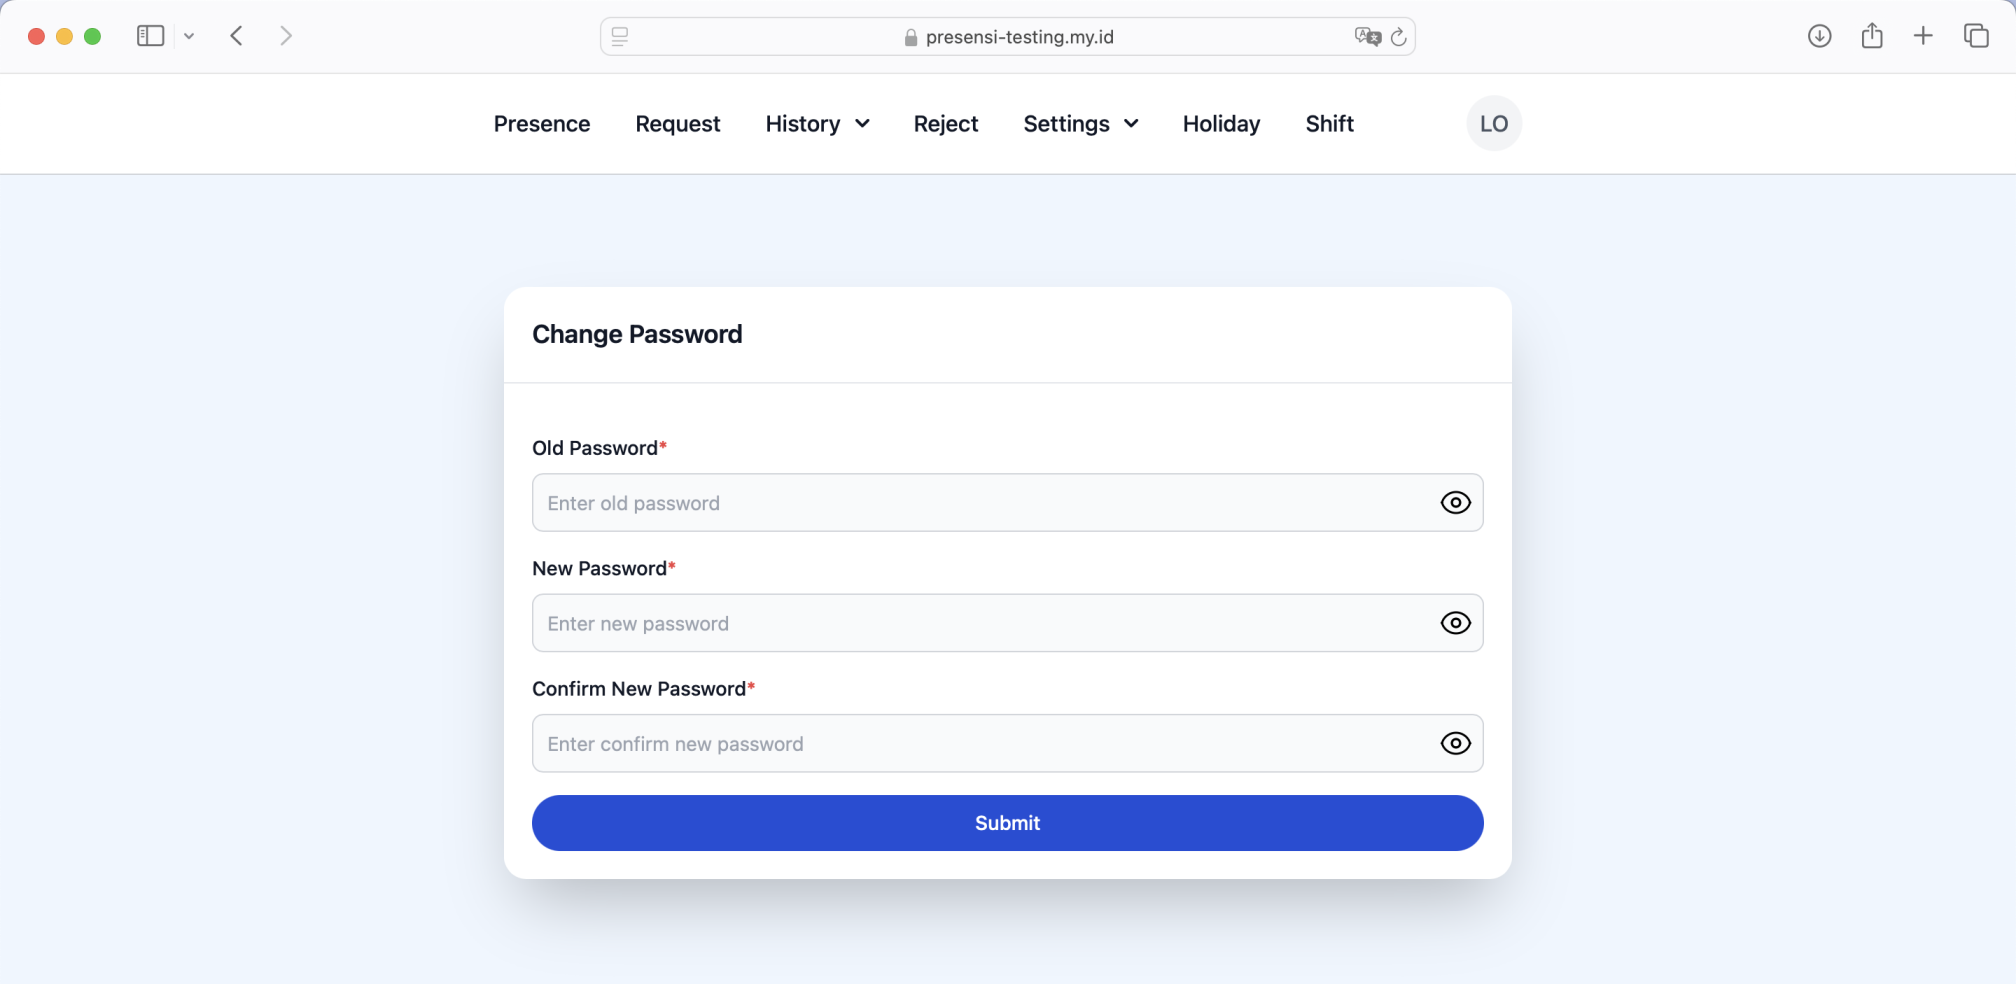
\includegraphics[width=8cm]{Gambar/bab3/user-manual/user-manual-halaman-change-password.png}
    	\caption{Halaman \textit{Change Password}}
    	\label{fig:user-manual-halaman-change-password}
        \end{figure}
        \FloatBarrier
    \end{enumerate}

    \item Melakukan \textit{Logout}
    \begin{enumerate}
        \item Melakukan \textit{login} pada aplikasi presensi \textit{online} yang terdapat pada \textbf{Manual \ref{item:melakukan-login}}.
        \item Menekan ikon profil pada \textit{navigation bar} yang terletak di paling atas, kemudian memilih tombol "\textit{Sign Out}". \textbf{\ref{fig:user-manual-tombol-sign-out-pada-navigation-bar}} menunjukkan tombol \textit{"Sign Out"} pada \textit{navigation bar}.
        \begin{figure}[!htbp]
    	\centering
    	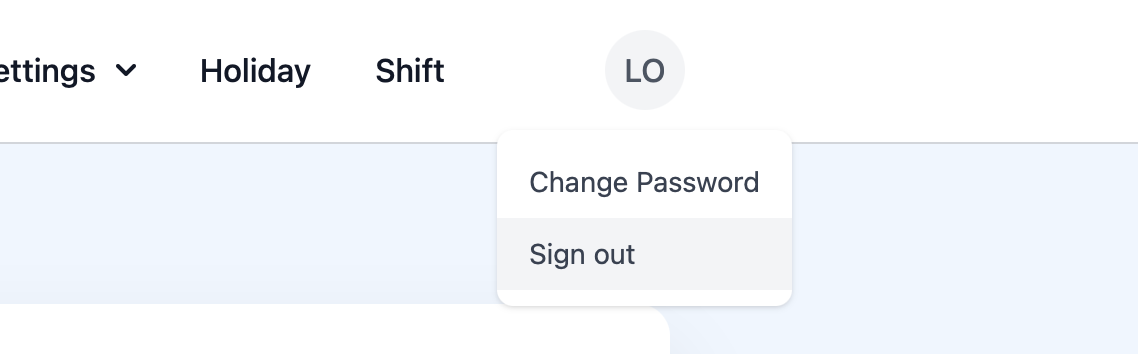
\includegraphics[width=8cm]{Gambar/bab3/user-manual/user-manual-navbar-sign-out.png}
    	\caption{Tombol \textit{Sign Out} Pada \textit{Navigation Bar}}
    	\label{fig:user-manual-tombol-sign-out-pada-navigation-bar}
        \end{figure}
        \FloatBarrier
        \item Halaman akan dialihkan ke halaman \textit{login}.
    \end{enumerate}
   
\end{enumerate}